\documentclass[aspectratio=169,9pt]{beamer}
%	***********
%	* PACKAGE *
%	***********
\usepackage{amsmath,amssymb,amsfonts,mathtools,graphicx,xcolor,bm,microtype,physics}
\usepackage{booktabs}
\usepackage{tabularx}
\usepackage{array}
\usepackage{makecell}
\usepackage{colortbl}
\usepackage{tikz,pgfplots}
\pgfplotsset{compat=1.18}
\usepackage[version=4]{mhchem}
\usepackage{libertine}
\usepackage[libertine]{newtxmath}
\DeclareMathSizes{9}{9}{7}{5}
\usefonttheme{professionalfonts}
\usetheme{default}
\beamertemplatenavigationsymbolsempty
\setbeamertemplate{headline}{}

% A restrained, high-contrast visual system for projection.
\definecolor{hfNavy}{HTML}{17324D}
\definecolor{hfBlue}{HTML}{1769AA}
\definecolor{hfTeal}{HTML}{007C83}
\definecolor{hfRed}{HTML}{B23A48}
\definecolor{hfOrange}{HTML}{D96C22}
\definecolor{hfGreen}{HTML}{2F7D4A}
\definecolor{hfPurple}{HTML}{9A7300}
\definecolor{hfViolet}{HTML}{775DA6}
\definecolor{hfInk}{HTML}{202A33}
\definecolor{hfPale}{HTML}{EDF2F6}

\setbeamercolor{normal text}{fg=hfInk,bg=white}
\setbeamercolor{structure}{fg=hfNavy}
\setbeamercolor{alerted text}{fg=hfRed}
\setbeamercolor{frametitle}{fg=white,bg=hfNavy}
\setbeamercolor{title}{fg=hfNavy}
\setbeamercolor{block title}{fg=white,bg=hfNavy}
\setbeamercolor{block body}{fg=hfInk,bg=hfPale}
\setbeamercolor{itemize item}{fg=hfTeal}
\setbeamercolor{itemize subitem}{fg=hfTeal}
\setbeamerfont{title}{size=\Huge,series=\bfseries}
\setbeamerfont{frametitle}{size=\large,series=\bfseries}
%\setbeamerfont{block title}{series=\bfseries}
\setbeamertemplate{blocks}[rounded][shadow=false]
\setbeamertemplate{itemize item}{\color{hfTeal}\raisebox{0.15ex}{\rule{0.55ex}{0.55ex}}}
\setbeamertemplate{itemize subitem}{\color{hfTeal}\raisebox{0.12ex}{\rule{0.45ex}{0.45ex}}}
\setbeamersize{text margin left=0.55cm,text margin right=0.55cm}
%\setbeamertemplate{frametitle}{%
%  \nointerlineskip
%  \begin{beamercolorbox}[wd=\paperwidth,ht=0.78cm,dp=0.22cm,leftskip=0.55cm,rightskip=0.55cm]{frametitle}
%    \usebeamerfont{frametitle}\insertframetitle
%  \end{beamercolorbox}%
%}
%\setbeamertemplate{footline}{%
%  \leavevmode%
%  \hbox{%
%    \begin{beamercolorbox}[wd=.82\paperwidth,ht=2.6ex,dp=1.1ex,leftskip=.55cm]{author in head/foot}%
%      \color{hfNavy}\insertshorttitle\hspace{0.7em}\textcolor{hfTeal}{/}\hspace{0.7em}\insertsectionhead
%    \end{beamercolorbox}%
%    \begin{beamercolorbox}[wd=.18\paperwidth,ht=2.6ex,dp=1.1ex,rightskip=.55cm plus1fil]{page number in head/foot}%
%      \color{hfNavy}\hfill\insertframenumber
%    \end{beamercolorbox}%
%  }%
%}

\usepackage{hyperref}
\hypersetup{
    colorlinks=true,
    linkcolor=hfTeal,
    filecolor=magenta,
    urlcolor=hfTeal,
    citecolor=hfPurple
}
\urlstyle{same}

%	***********
%	* PACKAGE *
%	***********

% energies
\newcommand{\Ec}{E_\text{c}}
\newcommand{\EHF}{E_\text{HF}}

% bold symbols
\newcommand{\br}{\boldsymbol{r}}
\newcommand{\bx}{\boldsymbol{x}}
\newcommand{\bc}{\boldsymbol{c}}
\newcommand{\bs}{\boldsymbol{s}}
\newcommand{\bR}{\boldsymbol{R}}
\newcommand{\bo}{\boldsymbol{o}}
\newcommand{\bA}{\boldsymbol{A}}
\newcommand{\bB}{\boldsymbol{B}}
\newcommand{\bC}{\boldsymbol{C}}
\newcommand{\bE}{\boldsymbol{E}}
\newcommand{\bG}{\boldsymbol{G}}
\newcommand{\bJ}{\boldsymbol{J}}
\newcommand{\bK}{\boldsymbol{K}}
\newcommand{\bP}{\boldsymbol{P}}
\newcommand{\bI}{\boldsymbol{1}}
\newcommand{\bU}{\boldsymbol{U}}
\newcommand{\bO}{\boldsymbol{0}}
\newcommand{\bS}{\boldsymbol{S}}
\newcommand{\bT}{\boldsymbol{T}}
\newcommand{\bF}{\boldsymbol{F}}
\newcommand{\bH}{\boldsymbol{H}}
\newcommand{\bV}{\boldsymbol{V}}
\newcommand{\bX}{\boldsymbol{X}}
\newcommand{\be}{\boldsymbol{e}}
\newcommand{\bepsilon}{\boldsymbol{\epsilon}}

% hat symbols
\newcommand{\hH}{\Hat{H}}
\newcommand{\hh}{\Hat{h}}
\newcommand{\hf}{\Hat{f}}
\newcommand{\hT}{\Hat{T}}
\newcommand{\hV}{\Hat{V}}
\newcommand{\hO}{\Hat{O}}
\newcommand{\hJ}{\Hat{J}}
\newcommand{\hK}{\chK}
\newcommand{\hS}{\Hat{S}}

% curly symbols
\newcommand{\chA}{\Hat{\mathcal{A}}}
\newcommand{\chO}{\Hat{\mathcal{O}}}
\newcommand{\chJ}{\Hat{\mathcal{J}}}
\newcommand{\chK}{\Hat{\mathcal{K}}}
\newcommand{\chH}{\Hat{\mathcal{H}}}
\newcommand{\chT}{\Hat{\mathcal{T}}}
\newcommand{\chV}{\Hat{\mathcal{V}}}
\newcommand{\chP}{\Hat{\mathcal{P}}}
\newcommand{\chS}{\Hat{\mathcal{S}}}

\newcommand{\cE}{\mathcal{E}}
\newcommand{\cJ}{\mathcal{J}}
\newcommand{\cK}{\mathcal{K}}

% colors and others
\newcommand{\mc}{\multicolumn}
\newcommand{\purple}[1]{\textcolor{hfPurple}{#1}}
\newcommand{\red}[1]{\textcolor{hfRed}{#1}}
\newcommand{\orange}[1]{\textcolor{hfOrange}{#1}}
\newcommand{\green}[1]{\textcolor{hfGreen}{#1}}
\newcommand{\blue}[1]{\textcolor{hfBlue}{#1}}
\newcommand{\violet}[1]{\textcolor{hfViolet}{#1}}
\newcommand{\pub}[1]{{\small\textcolor{hfPurple}{#1}}}

% brakets
\newcommand{\sbra}[1]{[ #1 |}
\newcommand{\sket}[1]{| #1 ]}
\newcommand{\sexpval}[1]{[ #1 ]}
\newcommand{\sbraket}[2]{[ #1 | #2 ]}
\newcommand{\smel}[3]{[ #1 | #2 | #3 ]}

\newcommand{\rbra}[1]{( #1 |}
\newcommand{\rket}[1]{| #1 )}
\newcommand{\rexpval}[1]{( #1 )}
\newcommand{\rbraket}[2]{( #1 | #2 )}
\newcommand{\rmel}[3]{( #1 | #2 | #3 )}

% shortcuts
\newcommand{\si}{\sigma}
\newcommand{\la}{\lambda}

\newcommand{\cre}[1]{\Hat{a}_{#1}^\dag}
\newcommand{\ani}[1]{\Hat{a}_{#1}}

%	*************
%	* HEAD DATA *
%	*************
	\title[HF Theory]{
		Hartree--Fock Theory
	} 
        \author[PF Loos]{Pierre-Fran\c{c}ois Loos}
        \date{ESQC 2026}
        \institute[CNRS@LCPQ]{
                Laboratoire de Chimie et Physique Quantiques (UMR 5626),
                Universit\'e de Toulouse, CNRS, UPS, Toulouse, France
        }
        \titlegraphic{
%                \vspace{0.2\textheight}
%                
\includegraphics[height=0.05\textwidth]{fig/UPS}
%                \hspace{0.2\textwidth}
%                
\includegraphics[height=0.05\textwidth]{fig/ERC}
%                \hspace{0.2\textwidth}
                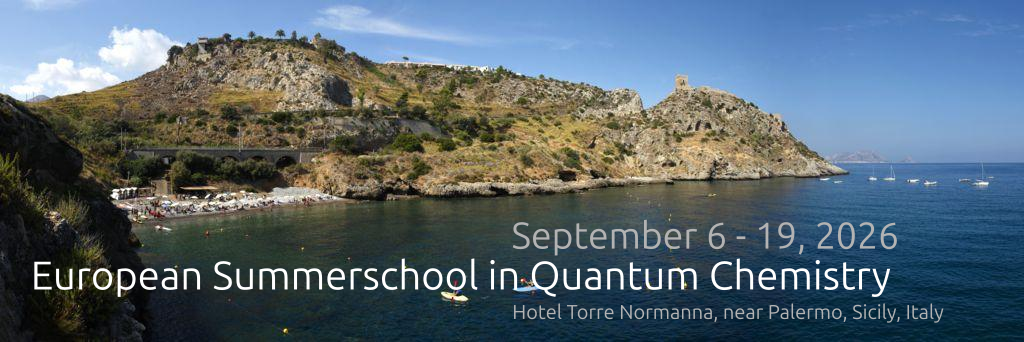
\includegraphics[width=0.7\textwidth]{fig/front}
%                \hspace{0.2\textwidth}
%                
\includegraphics[height=0.05\textwidth]{fig/CNRS}
        }
        
\begin{document}

%-----------------------------------------------------
%%%	TITLE		%%%
%-----------------------------------------------------
\begin{frame}
	\titlepage
\end{frame}

%%% SLIDE X %%%
%\begin{frame}{How to perform a HF calculation in practice?}
%	\begin{columns}
%		\begin{column}{0.7\textwidth}
%			\begin{block}{The SCF algorithm for Hartree-Fock (HF) calculations (p.~146)}
%				\begin{enumerate}
%					\item \orange{Specify molecule} $\{\bR_A\}$ and $\{Z_A\}$ and \violet{basis set} $\{\phi_\mu\}$ 
%					\item Calculate integrals $S_{\mu \nu}$, $H_{\mu \nu}$ and $\braket{\mu \nu}{\lambda \sigma}$
%					\item Diagonalize $\bS$ and compute $\bX = \bS^{-1/2}$
%					\item Obtain \alert{guess density matrix} for $\bP$
%					\begin{enumerate}
%						\item[1.] Calculate $\bJ$ and $\bK$, then $\bF = \bH + \bJ + \bK$
%						\item[2.] Compute $\bF' = \bX^\dag \cdot  \bF \cdot  \bX$
%						\item[3.] Diagonalize $\bF'$ to obtain $\bC'$ and $\bE$
%						\item[4.] Calculate $\bC= \bX \cdot  \bC'$
%						\item[5.] Form a \blue{new density matrix} $\bP = \bC \cdot \bC^\dag$
%						\item[6.] \alert{Am I converged?} If not go back to 1.
%					\end{enumerate}
%					\item Calculate stuff that you want, like $\EHF$ for example
%				\end{enumerate}
%			\end{block}
%		\end{column}
%		\begin{column}{0.3\textwidth}
%			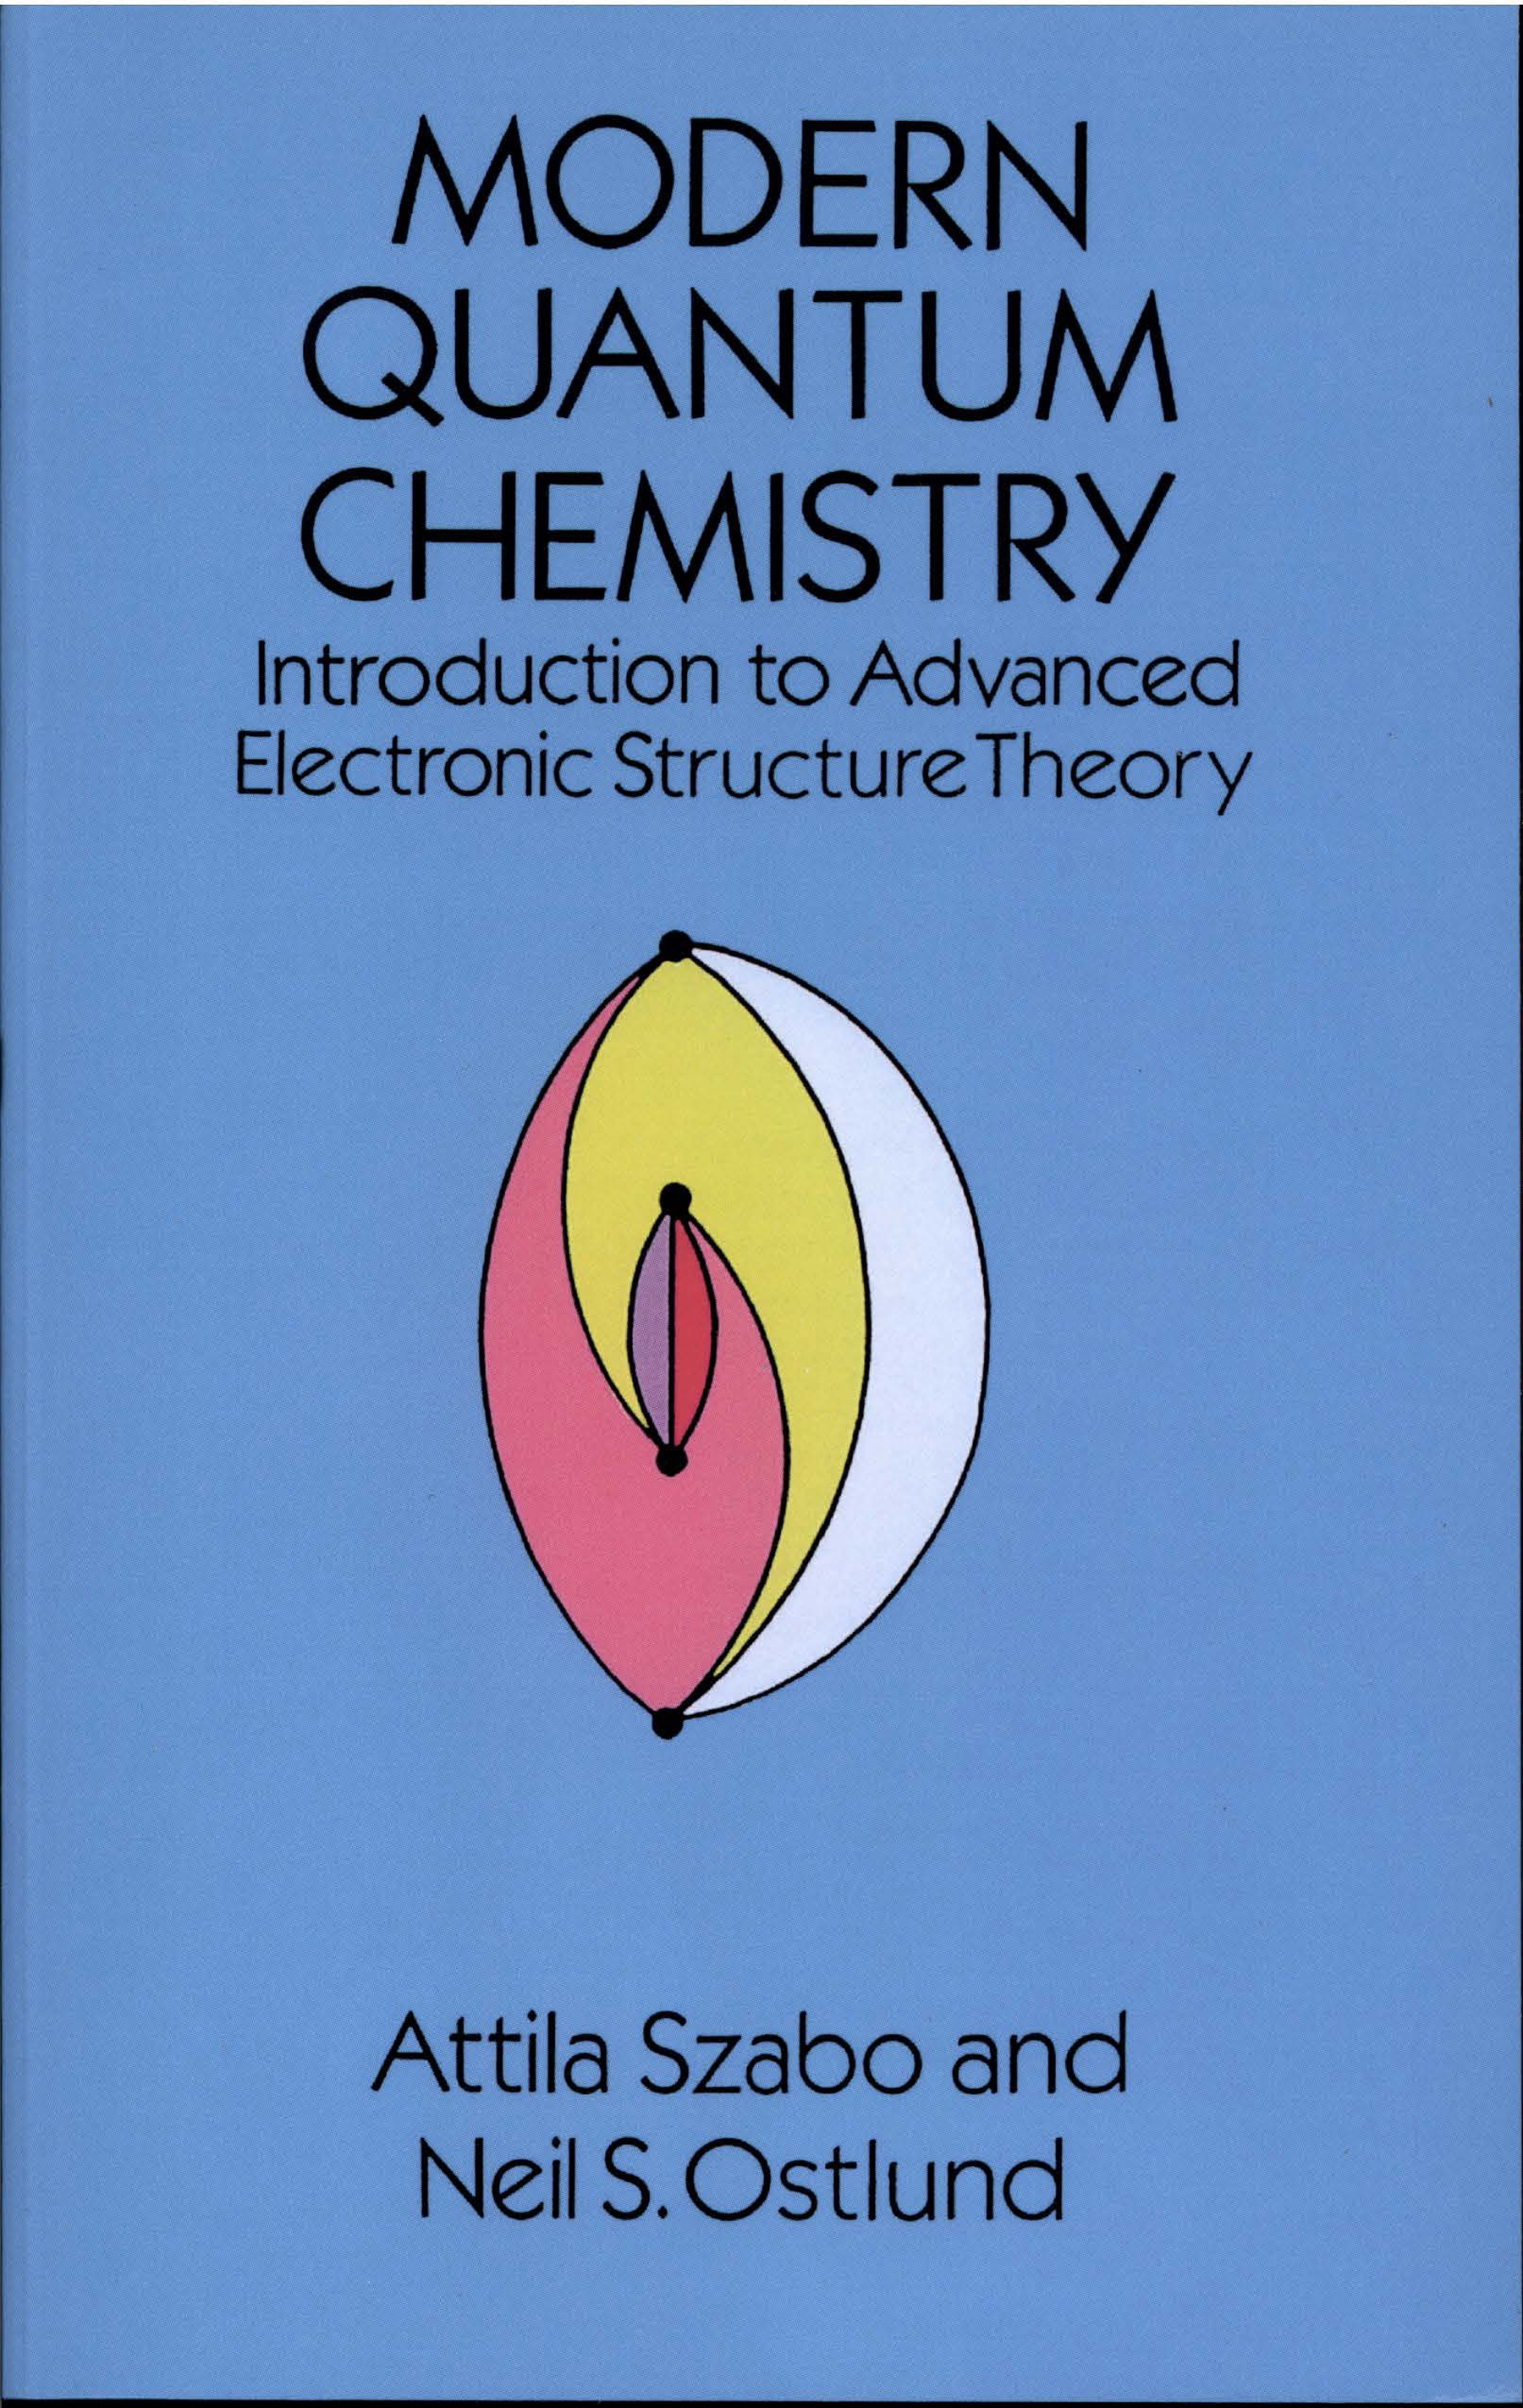
\includegraphics[width=\textwidth]{fig/Szabo}
%		\end{column}
%	\end{columns}
%\end{frame}

\begin{frame}{Szabo's and Ostlund's book}
	\begin{center}
		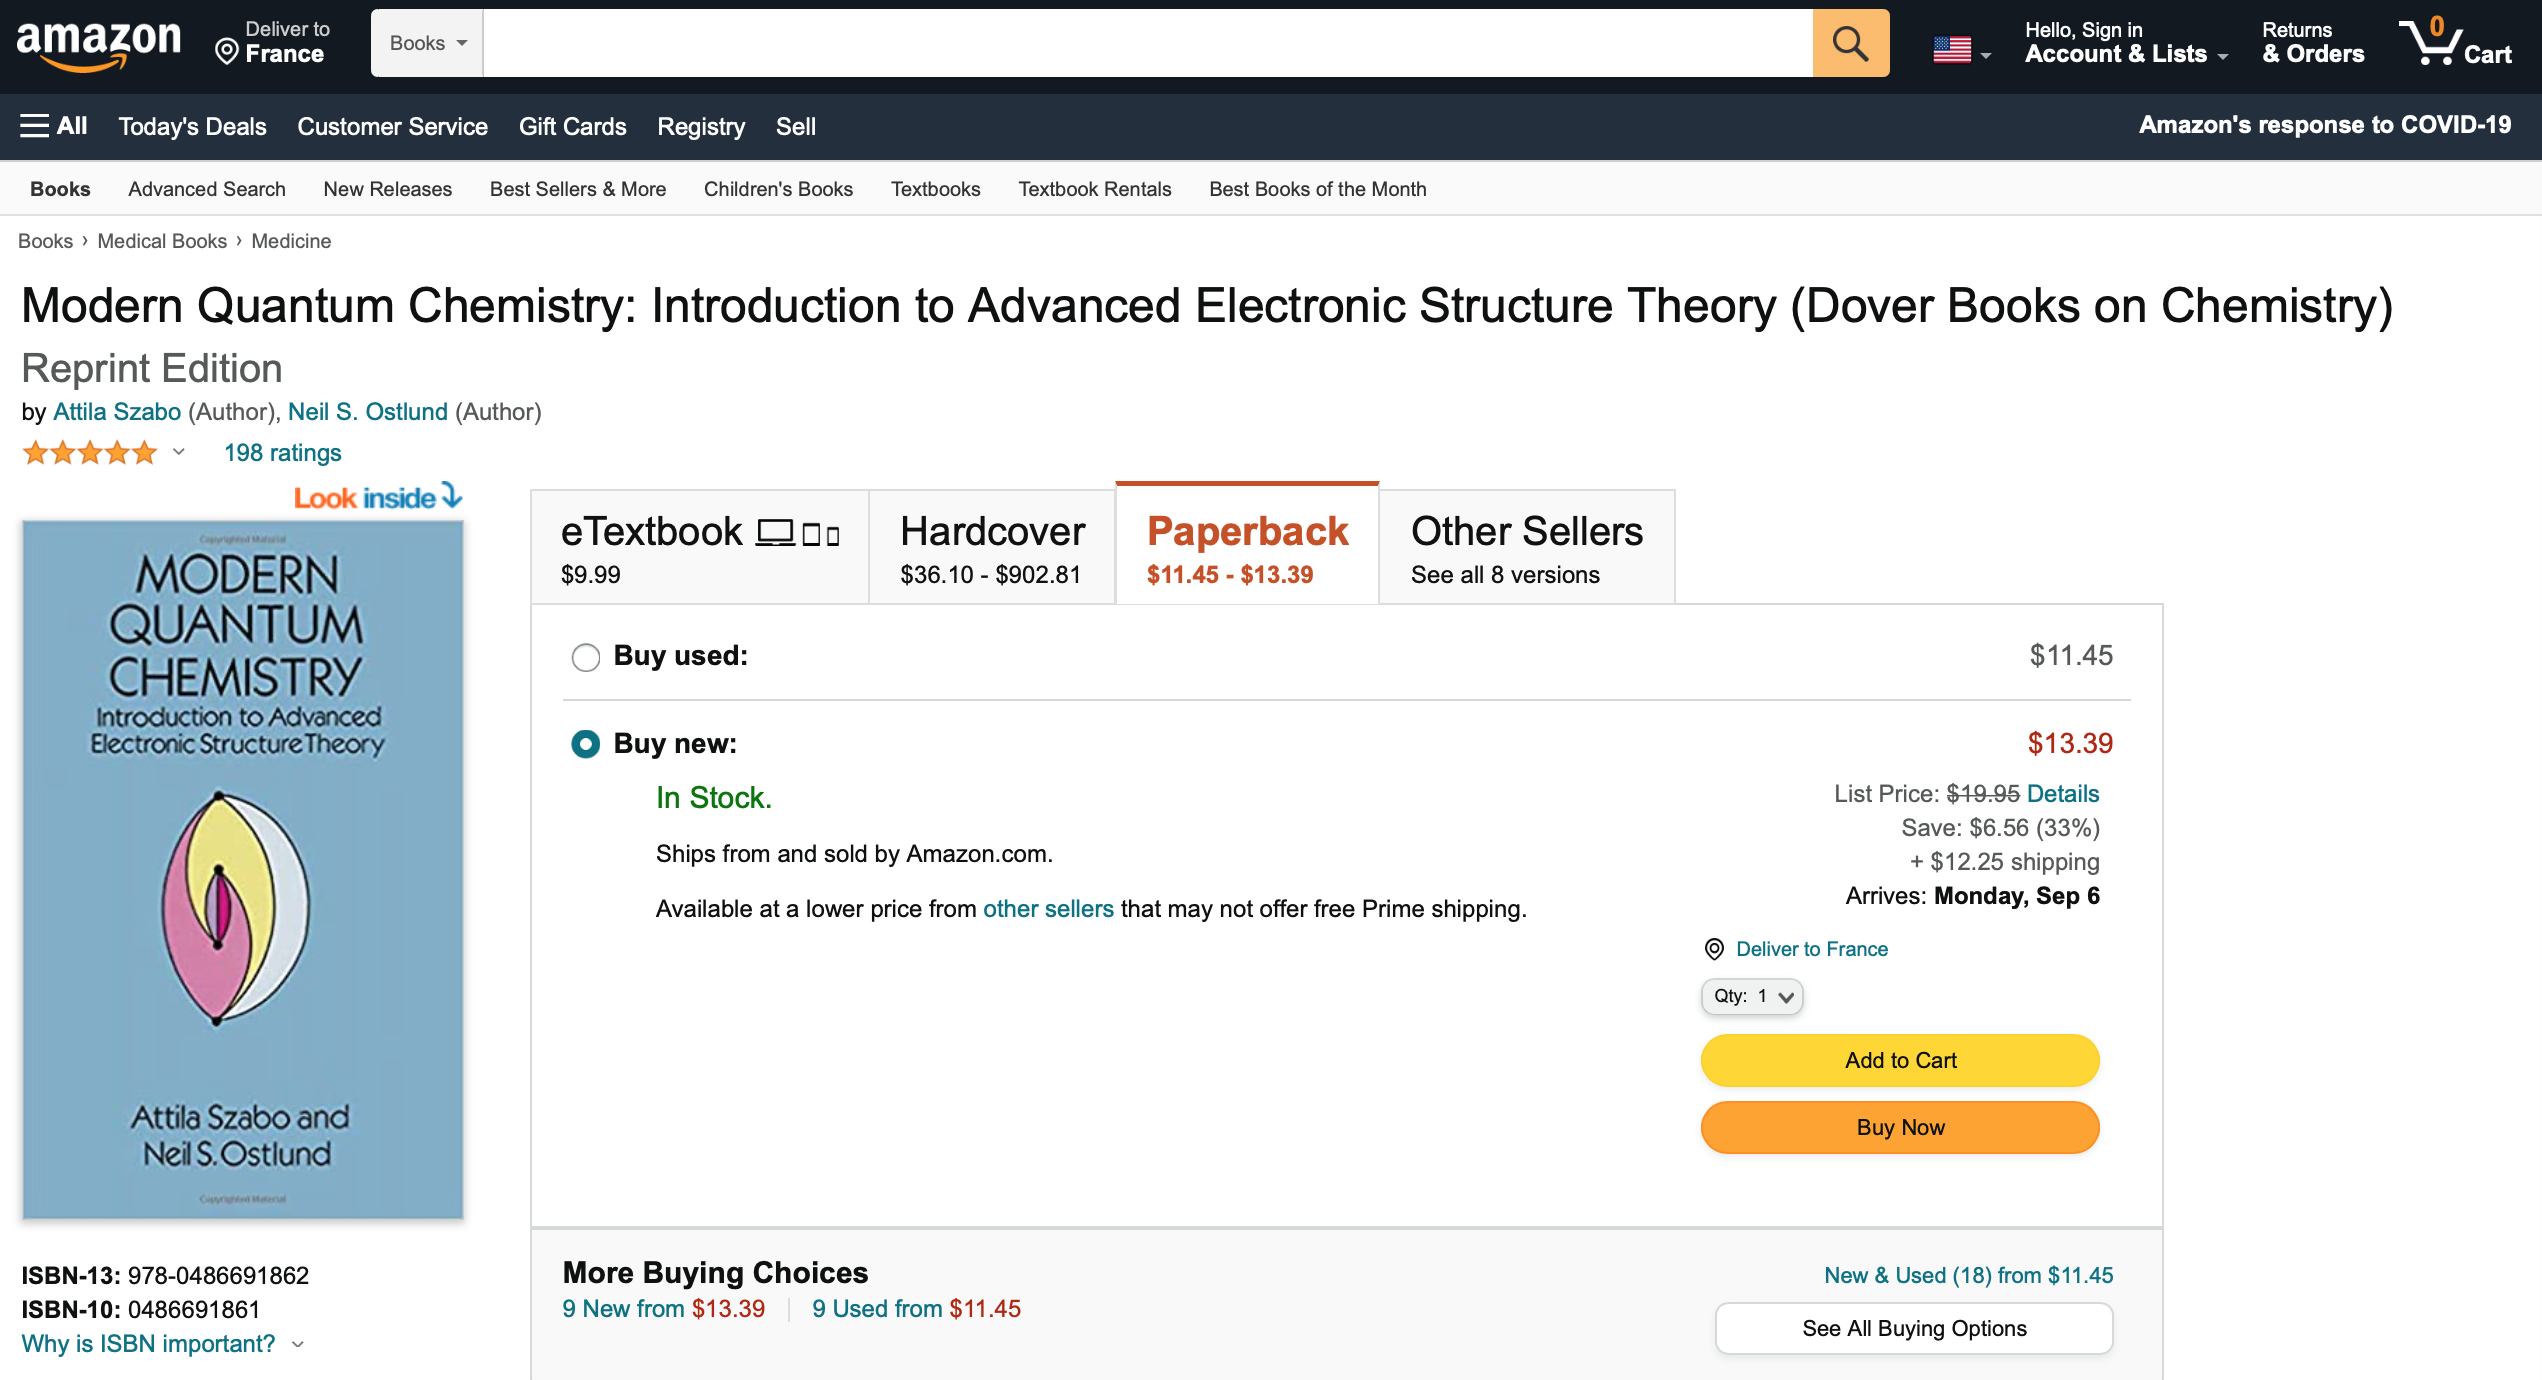
\includegraphics[width=\textwidth]{fig/amazon}
	\end{center}
\end{frame}

%-----------------------------------------------------
\section{The electronic problem}
%-----------------------------------------------------
%-----------------------------------------------------
\subsection{Motivations}
%-----------------------------------------------------
\begin{frame}{Motivations \& Assumptions}
	\begin{itemize}
		\item We consider the \alert{time-independent} Schr\"odinger equation
		\bigskip
		\item Hartree-Fock (HF) is an \alert{ab initio method}: it contains no empirical parameters, apart from the choice of basis set
		\bigskip
		\item We neglect \alert{relativistic effects}
		\bigskip
		\item HF is a \alert{mean-field approximation}, i.e., interactions are taken into account in an average fashion
		\bigskip
		\item \alert{HF is the starting point for much of electronic-structure theory}
	\end{itemize}
\end{frame}

%-----------------------------------------------------
\subsection{Born-Oppenheimer}
%-----------------------------------------------------
\begin{frame}{The Hamiltonian}
	In the \alert{Schr\"odinger equation}
	\begin{equation}
		\chH \Phi(\{\br_i\},\{\bR_A\}) = \cE \Phi(\{\br_i\},\{\bR_A\})
	\end{equation}
	the \alert{total Hamiltonian} is 
	\begin{equation}
		\boxed{
		\chH = \green{\chT_\text{n}} +  \blue{\chT_\text{e}} +  \orange{\chV_\text{ne}} +  \alert{\chV_\text{ee}} +  \violet{\chV_\text{nn}}
		}
	\end{equation}
	\begin{block}{What are all these terms?}
		\begin{itemize}
			\item \green{$\chT_\text{n}$} is the \green{kinetic energy of the nuclei}
			\bigskip
			\item \blue{$\chT_\text{e}$} is the \blue{kinetic energy of the electrons}
			\bigskip
			\item \orange{$\chV_\text{ne}$} is the \orange{Coulomb attraction between nuclei and electrons}
			\bigskip
			\item \alert{$\chV_\text{ee}$} is the \alert{Coulomb repulsion between electrons}
			\bigskip
			\item \violet{$\chV_\text{nn}$} is the \violet{Coulomb repulsion between nuclei}
		\end{itemize}
	\end{block}
\end{frame}

\begin{frame}{Hamiltonian terms in atomic units}
	\begin{columns}
		\begin{column}{0.4\textwidth}
			\begin{block}{In atomic units ($m = e = \hbar = 1$)}
				\begin{subequations}
				\begin{align}
					& \green{\chT_\text{n}} = - \sum_{A=1}^{M} \frac{\laplacian_A}{2 M_A} 
					 \\	
					&  \blue{\chT_\text{e}} =  - \sum_{i=1}^{N} \frac{\laplacian_i}{2} 
					\\
					&  \orange{\chV_\text{ne}} = - \sum_{A=1}^{M} \sum_{i=1}^N \frac{Z_A}{r_{iA}} 
					 \\
					& \alert{\chV_\text{ee}} =  \sum_{i<j}^N \frac{1}{r_{ij}} 
					 \\
					&  \violet{\chV_\text{nn}} = \sum_{A<B}^{M} \frac{Z_A Z_B}{R_{AB}} 
				\end{align}
				\end{subequations}
			\end{block}
		\end{column}
		\begin{column}{0.6\textwidth}
			\begin{itemize}
				\item $\laplacian$ is the \green{Laplace operator} (or Laplacian)
				\bigskip
				\item $M_A$ is the \orange{mass} of nucleus $A$
				\bigskip
				\item $Z_A$ is the \violet{charge} of nucleus $A$
				\bigskip
				\item $r_{iA}$ is the \red{distance} between electron $i$ and nucleus $A$
				\bigskip
				\item $r_{ij}$ is the \red{distance} between electrons $i$ and $j$
				\bigskip
				\item $R_{AB}$ is the \red{distance} between nuclei $A$ and $B$
			\end{itemize}
		\end{column}
	\end{columns}
\end{frame}

\begin{frame}{Molecular coordinate system}
	\begin{center}
		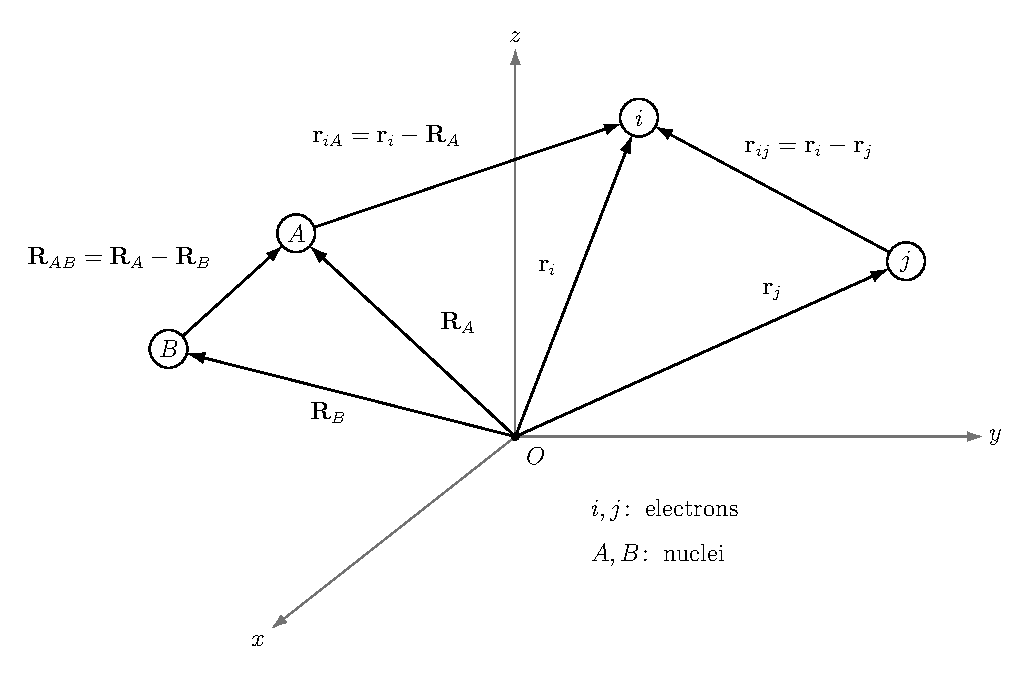
\includegraphics[width=0.7\textwidth]{fig/coord}
	\end{center}
\end{frame}

\begin{frame}{The Born-Oppenheimer approximation}
	\begin{block}{Born-Oppenheimer approximation = decoupling nuclei and electrons}
		Because $M_A \gg 1$, the nuclear coordinates are ``parameters'' $\Rightarrow$ \red{potential energy surface (PES)}
		\begin{equation}
			\Phi(\{\br_i\},\{\bR_A\}) = \Phi_\text{nucl}(\{\bR_A\}) \Phi_\text{elec}(\{\br_i\},\{\bR_A\})
			\qq{with}
			\cE_\text{tot} = \cE_\text{elec} + \sum_{A<B}^{M} \frac{Z_A Z_B}{R_{AB}} 
		\end{equation}
	\end{block}
	\begin{block}{Nuclear Hamiltonian}
		The \alert{nuclear Hamiltonian} is
		\begin{equation}
			\chH_\text{nucl} \Phi_\text{nucl} = \cE_\text{nucl} \Phi_\text{nucl}
			\qq{with}
			\boxed{\chH_\text{nucl} = \green{\chT_\text{n}} + \violet{\chV_\text{nn}}}
		\end{equation}
		It describes the vibration, rotation and translation of the molecules
	\end{block}
	\begin{block}{Electronic Hamiltonian}
		The \alert{electronic Hamiltonian} is
		\begin{equation}
			\chH_\text{elec} \Phi_\text{elec} = \cE_\text{elec} \Phi_\text{elec}
			\qq{with}
			\boxed{\chH_\text{elec} = \blue{\chT_\text{e}} +  \orange{\chV_\text{ne}} +  \alert{\chV_\text{ee}}}
		\end{equation}
	\end{block}
\end{frame}

%\begin{frame}{Separability of the Schr\"odinger equation}
%	\begin{block}{Problem:}
%	\textit{\violet{``Assuming that $\hH = \hH_A + \hH_B$ with $\hH_A \Psi_A = E_A \Psi_A$ and $\hH_B \Psi_B = E_B \Psi_B$, find the expression of $\Psi$ and $E$ such that $\hH \Psi = E \Psi$''}}
%	\end{block}
%	\pause
%	\begin{block}{Solution}
%	Let's try $\Psi = \Psi_A \Psi_B$ and see if we're lucky. 
%	\\
%	Then,
%	\begin{equation*}
%	\begin{split}
%		\hH \Psi 
%		& = ( \hH_A + \hH_B) \Psi_A \Psi_B 
%		\\
%		& = \hH_A \Psi_A \Psi_B + \hH_B \Psi_A \Psi_B 
%		\\
%		& = E_A \Psi_A \Psi_B + E_B \Psi_A \Psi_B 
%		\\
%		& = \underbrace{(E_A + E_B)}_{E} \underbrace{\Psi_A \Psi_B}_{\Psi}
%	\end{split}
%	\end{equation*}
%	\end{block}
%\end{frame}


%-----------------------------------------------------
\subsection{Pauli}
%-----------------------------------------------------

\begin{frame}{Spin of the electron}
	We are interested in \alert{electrons}, which are \alert{fermions} $\Rightarrow$ \alert{Pauli exclusion principle} (see next slide)
	\begin{block}{Spin functions: $\ket{\omega} = \ket{s,m_s}	\quad	s^2 \ket{s,m_s} = s(s+1) \ket{s,m_s}	\quad	s_z \ket{s,m_s} = m_s \ket{s,m_s}$}
		\centering
		$ \ket{\red{\alpha}} = \ket{\frac{1}{2},+\frac{1}{2}}$ = \red{spin-up} electron 
		$\qquad$ 
		$\ket{\blue{\beta}}= \ket{\frac{1}{2},-\frac{1}{2}}$ = \blue{spin-down} electron\\
		\begin{align}
			\int \red{\alpha}^*(\omega) \blue{\beta}(\omega) \dd{\omega} & = \int \blue{\beta}^*(\omega) \red{\alpha}(\omega) \dd{\omega} & = 0 	
			& & 
			\int \red{\alpha}^*(\omega) \red{\alpha}(\omega) \dd{\omega} & = \int \blue{\beta}^*(\omega) \blue{\beta}(\omega) \dd{\omega} & = 1 	
			\\
			\braket{\red{\alpha}}{\blue{\beta}} & = \braket{\blue{\beta}}{\red{\alpha}} & = 0	
			& &  	
			\braket{\red{\alpha}}{\red{\alpha}} & = \braket{\blue{\beta}}{\blue{\beta}} & = 1
		\end{align}
	\end{block}
	\bigskip
	The \violet{composite variable $\bx$} combines \orange{spin ($\omega$)} and \red{spatial ($\br$)} coordinates: $\boxed{\violet{\bx} = (\orange{\omega},\red{\br})}$
	\begin{block}{Pauli exclusion principle}
		\begin{equation}
			\chH_\text{elec} \Phi(\bx_1,\bx_2,\ldots,\bx_N) = \cE_\text{elec} \Phi(\bx_1,\bx_2,\ldots,\bx_N)
		\end{equation}
		\begin{equation}
			\Phi(\bx_1,\ldots,\bx_i,\ldots,\bx_j,\ldots,\bx_N) = - \Phi(\bx_1,\ldots,\bx_j,\ldots,\bx_i,\ldots,\bx_N)
		\end{equation}		
	\end{block}
\end{frame}

\begin{frame}{Bosons vs Fermions}
%	\begin{block}{Problem:}
%		\violet{\textit{``Show that, for a system of two fermions, the wave function vanishes when they are at the same point in spin-space''}}
%	\end{block}
%	\pause
	\begin{block}{Symmetry vs Antisymmetry}
		Indistinguishable particles means 
		\begin{equation}
			\boxed{\abs{\Psi(\bx_1,\bx_2)}^2 = \abs{\Psi(\bx_2,\bx_1)}^2  \qq{$\Rightarrow$}  \Psi(\bx_1,\bx_2) = \alert{\pm} \Psi(\bx_2,\bx_1)}
		\end{equation}
		\\
		\bigskip
%		\pause
		\violet{Bosons} mean \violet{$\Psi(\bx_1,\bx_2) = \Psi(\bx_2,\bx_1)$} and \orange{Fermions} mean \orange{$\Psi(\bx_1,\bx_2) = -\Psi(\bx_2,\bx_1)$}
		\\
		\bigskip
		Let's put them at the same spot, i.e. \alert{$\bx = \bx_1 = \bx_2$}
		\begin{equation}
			\text{\orange{For Fermions, }} \Psi(\bx,\bx) = - \Psi(\bx,\bx)	\qq{$\Rightarrow$} 	\boxed{\Psi(\bx,\bx) = 0}
		\end{equation}
		\alert{The wave function vanishes: this is the origin of the Fermi (exchange) hole.}
	\end{block}
\end{frame}

\begin{frame}{Antisymmetry}
	\begin{block}{Problem:}
		\violet{\textit{``Given two one-electron functions $\chi_1(\bx)$ and $\chi_2(\bx)$, could you construct a two-electron (fermionic) wave function $\Psi(\bx_1,\bx_2)$?''}}
	\end{block}
	\pause
	\begin{block}{Solution}
		A possible solution is
		\begin{equation}
			\Psi(\bx_1,\bx_2) = \chi_1(\bx_1) \chi_2(\bx_2) -  \chi_2(\bx_1) \chi_1(\bx_2)
		\end{equation}
		This has been popularized by Slater:
		\begin{equation}
			\boxed{
			\Psi(\bx_1,\bx_2) = 
			\begin{vmatrix}
				\chi_1(\bx_1)	&	\chi_2(\bx_1)		\\
				\chi_1(\bx_2)	&	\chi_2(\bx_2)		\\
			\end{vmatrix}
			= \chi_1(\bx_1) \chi_2(\bx_2) -  \chi_2(\bx_1) \chi_1(\bx_2)
			}
		\end{equation}
		\alert{This is called a Slater determinant!}
		\\
		\bigskip
		A wave function of the form \green{$\Psi(\bx_1,\bx_2) = \chi_1(\bx_1) \chi_2(\bx_2)$} is called a \green{Hartree product}
	\end{block}
\end{frame}

%-----------------------------------------------------
\subsection{Hartree-Fock wave function}
%-----------------------------------------------------
\begin{frame}{The HF wave function}
	\begin{block}{A Slater determinant}
		\begin{equation}
			\begin{split}
				\Psi_\text{HF}(\bx_1,\bx_2,\ldots,\bx_N) 
				& = \frac{1}{\sqrt{N!}}
				\begin{vmatrix}
				\chi_1(\bx_1)	&	\chi_2(\bx_1)	&	\cdots	&	\chi_N(\bx_1)	\\
				\chi_1(\bx_2)	&	\chi_2(\bx_2)	&	\cdots	&	\chi_N(\bx_2)	\\
				\vdots			&	\vdots			&	\ddots	&	\vdots			\\
				\chi_1(\bx_N)	&	\chi_2(\bx_N)	&	\cdots	&	\chi_N(\bx_N)	\\
				\end{vmatrix}
				\equiv \ket{ \chi_1(\bx_1) \chi_2(\bx_2) \ldots \chi_N(\bx_N) }
				\\
				& = \blue{\chA}\qty[\chi_1(\bx_1) \chi_2(\bx_2) \ldots \chi_N(\bx_N)]
				= \blue{\chA}\green{\Pi(\bx_1,\bx_2,\ldots,\bx_N)}
			\end{split}	
		\end{equation}
		\begin{itemize}
			\item $\blue{\chA}$ is called the \blue{antisymmetrizer}
			\item $\green{\Pi(\bx_1,\bx_2,\ldots,\bx_N)}$ is a \green{Hartree product}
			\item \alert{The many-electron wave function $\Psi_\text{HF}(\bx_1,\bx_2,\ldots,\bx_N) $ is an antisymmetrized product of one-electron functions}
		\end{itemize}
	\end{block}
\end{frame}

\begin{frame}{Spin and spatial orbitals}
	\small
	\begin{equation}
		\chi_p(\bx) = \red{\underbrace{\sigma(\omega)}_{\text{spin}}} \blue{\underbrace{\psi_p(\br)}_{\text{spatial}}}
		\qq{with}
		\red{\sigma(\omega)} =
		\begin{cases}
			\alpha(\omega) 
			\\
			\beta(\omega)
		\end{cases}
		\qand
		\blue{\psi_p(\br)} = \underbrace{\sum_\mu^K C_{\mu p} \green{\phi_{\mu}(\br)}}_{\text{\green{LCAO}}}
	\end{equation}
%	These are \alert{restricted spin orbitals} $\Rightarrow$ \violet{Restricted Hartree-Fock = \textbf{RHF}}
	\begin{block}{The spin orbitals are orthogonal}
		\begin{equation}
			\braket{ \chi_p }{ \chi_q } = \int \chi_p^*(\bx) \chi_q(\bx) \dd{\bx} = \delta_{pq} 
			=
			\begin{cases}
				1	&	\text{if $p=q$}		\\
				0	&	\text{otherwise}		\\
			\end{cases}
		\end{equation}
	\end{block}
	\begin{block}{The spatial orbitals are orthogonal}
		\begin{equation}
			\braket{ \psi_p }{ \psi_q }  = \int \psi_p^*(\br) \psi_q(\br) \dd{\br} = \delta_{pq} 
%			\text{ \green{ = Kronecker delta}}
		\end{equation}
	\end{block}
	\begin{block}{The basis functions \alert{are, a priori, not} orthogonal}
		\begin{equation}
			\braket{ \phi_\mu }{ \phi_\nu } = \int \phi_\mu^*(\br) \phi_\nu(\br) \dd{\br} = S_{\mu \nu} 
			\text{ \green{ = Overlap matrix}}	
		\end{equation}
	\end{block}
\end{frame}
\begin{frame}{Orbital spaces and index conventions}
	\begin{block}{Orbitals}
		\begin{itemize}
			\item $\{ \phi_{\mu} | \mu=1,\ldots,K \}$ are \green{basis functions} or \green{atomic orbitals (AOs)}
			\item $\{ \psi_p | p=1,\ldots,K \}$ are \violet{spatial orbitals} or \violet{molecular orbitals (MOs)}
			\item $\{ \chi_p | p=1,\ldots,2K \}$ are \orange{spin orbitals}
		\end{itemize}
	\end{block}
	\begin{block}{Indices}
		\begin{itemize}
			\item With $K$ \green{basis functions}, one can create $K$ \violet{spatial orbitals} and $2K$ \orange{spin orbitals} $\Rightarrow$ \red{indices $p,q,r,s,\ldots$} 
			\item $N$ \orange{spin orbitals} are \red{occupied} $\Rightarrow$ \red{indices $i,j,k,l,\ldots$} 
			\item $2K-N$ \orange{spin orbitals} are \red{unoccupied/vacant} $\Rightarrow$ \red{indices $a,b,c,d,\ldots$}
		\end{itemize}
	\end{block}
	\begin{block}{Closed vs Open}
		\begin{itemize}
			\item When a system has \red{$2$ electrons in each orbital}, it is called a \red{closed-shell} system 
			\item Otherwise, it is called an \red{open-shell} system 
			\item For the ground state of a closed shell, the first $N/2$ spatial orbitals are \red{doubly-occupied} and the last $K-N/2$ are \red{vacant}
%			\bigskip
%			\item The MOs are built as \green{linear combinations of AOs (LCAO)}
%			\item The coefficients $C_{\mu i}$ are determined from the \alert{HF equations} using the \violet{variational principle}
		\end{itemize}
	\end{block}
\end{frame}

\begin{frame}{Restricted vs Unrestricted Hartree-Fock}
	\begin{columns}
	\begin{column}{0.65\textwidth}
	\begin{block}{Restricted formalism}
		\begin{itemize}
			\item \alert{Restricted HF (RHF)} is made to describe \alert{closed-shell systems}
			\begin{equation}
				\chi_p^\text{RHF}(\bx) 
				= 
				\begin{cases}
					\red{\alpha(\omega)} \psi_p(\br)
					\\
					\blue{\beta(\omega)} \psi_p(\br)
				\end{cases}
				= 
				\begin{cases}
					\red{\psi_p(\br)}
					\\
					\blue{\Bar{\psi}_p(\br)}
				\end{cases}
			\end{equation}
			\item RHF does {\bf not} describe \alert{open-shell systems}
		\end{itemize}
	\end{block}
	\begin{block}{Unrestricted formalism}
		\begin{itemize}
			\item For open-shell systems, one can use \alert{unrestricted HF (UHF)}
			\begin{equation}
				\chi_p^\text{UHF}(\bx) 
				= 
				\begin{cases}
					\alpha(\omega) \red{\psi_p^\alpha(\br)}
					\\
					\beta(\omega) \blue{\psi_p^\beta(\br)}
				\end{cases}
			\end{equation}
			\item UHF does break spin symmetry!
			\item \green{Restricted open-shell Hartree--Fock (ROHF)} retains shared spatial orbitals; we will not discuss it here
		\end{itemize}
	\end{block}
	\end{column}
	\begin{column}{0.35\textwidth}
		\center
		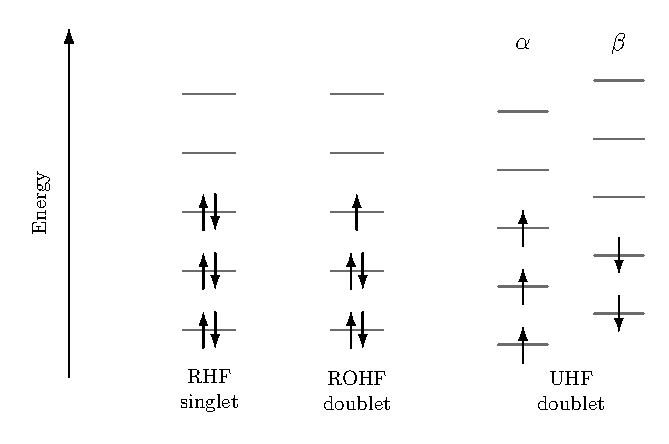
\includegraphics[width=\textwidth]{fig/RHF_UHF}
	\end{column}
	\end{columns}
\end{frame}



%-----------------------------------------------------
\section{HF approximation}
%-----------------------------------------------------
%-----------------------------------------------------
\subsection{HF energy}
%-----------------------------------------------------
\begin{frame}{The Hartree-Fock energy}
	\begin{block}{HF energy}
		\begin{equation}
			\boxed{\EHF = \mel{\Psi_\text{HF}}{\chH_\text{elec} + \violet{\chV_\text{nn}}}{\Psi_\text{HF}}}
			\qq{where}
			\chH_\text{elec} = \blue{\chT_\text{e}} +  \orange{\chV_\text{ne}} +  \alert{\chV_\text{ee}} 
		\end{equation}
	\end{block}
	\begin{block}{One-electron Hamiltonian (or core Hamiltonian)}
		\begin{equation}
			\chO_1 = \blue{\chT_\text{e}} +  \orange{\chV_\text{ne}} = \sum_{i=1}^N \hh(\bx_i)	
			\qq{where}	
			\hh(\bx_i) = -\frac{\laplacian_i}{2} - \sum_{A=1}^{M} \frac{Z_A}{r_{iA}} 
		\end{equation}
	\end{block}
	\begin{block}{Two-electron Hamiltonian (electron-electron repulsion)}
		\begin{equation}
			\chO_2 = \alert{\chV_\text{ee}} = \sum_{i<j}^N \frac{1}{r_{ij}} 
		\end{equation}
	\end{block}
\end{frame}

\begin{frame}{One-electron contributions to the HF energy}
	\begin{block}{Electronic Hamiltonian}
	\begin{equation}
		\boxed{\chH_\text{elec} = \sum_{i=1}^N \hh(\bx_i) + \sum_{i<j}^N \frac{1}{r_{ij}}}
	\end{equation}	
	\end{block}	
	\begin{block}{Nuclear repulsion}
			\begin{equation} 
				\mel{ \Psi_\text{HF} }{\violet{\chV_\text{nn}} }{ \Psi_\text{HF} } = \violet{V_\text{nn}} \braket{ \Psi_\text{HF} }{ \Psi_\text{HF} } = \violet{V_\text{nn}}
			\end{equation}
	\end{block}
	\begin{block}{Core Hamiltonian}
			\begin{equation} 
				\mel{ \Psi_\text{HF} }{ \chO_1 }{ \Psi_\text{HF} }  = \sum_{i=1}^N \mel{ \chi_i(\bx_1) }{ \hh(\bx_1) }{ \chi_i(\bx_1) } = \sum_{i=1}^N h_{ii}
			\end{equation}
	\end{block}
\end{frame}


\begin{frame}{Two-electron contributions to the HF energy}
	\begin{block}{Two-electron Hamiltonian:}
			\begin{equation}
			\begin{split} 
				\mel{ \Psi_\text{HF} }{ \chO_2 }{ \Psi_\text{HF} }  	
				& = \sum_{i<j}^N \qty[ \mel{ \chi_i(\bx_1) \chi_j(\bx_2) }{ r_{12}^{-1} }{ \chi_i(\bx_1) \chi_j(\bx_2) } - \mel{ \chi_i(\bx_1) \chi_j(\bx_2) }{ r_{12}^{-1} }{ \chi_j(\bx_1) \chi_i(\bx_2) } ]
				\\
				& = \sum_{i<j}^N \qty( \underbrace{\cJ_{ij}}_{\text{\green{Coulomb}}} - \underbrace{\cK_{ij}}_{\text{\red{Exchange}}} ) = \frac{1}{2} \sum_{i=1}^N \sum_{j=1}^N \qty( \cJ_{ij} - \cK_{ij} ) \qq{because} \alert{\boxed{\cJ_{ii} = \cK_{ii}}}
			\end{split}
			\end{equation}
	\end{block}
	\begin{block}{HF energy:}
			\begin{equation}
				\boxed{\EHF = \sum_{i=1}^N h_{ii} +\sum_{i<j}^N (\cJ_{ij} - \cK_{ij}) + \violet{V_\text{nn}} }
			\end{equation}
	\end{block}
\end{frame}

\begin{frame}{Coulomb operator}
	\begin{block}{Coulomb operator}
			\begin{equation}
			\begin{split}
				 \chJ_{\green{j}}(\blue{\bx_1}) \ket{ \chi_{\purple{i}}(\blue{\bx_1}) } 
				 & = \mel{ \chi_{\green{j}}(\red{\bx_2}) }{ r_{\blue{1}\red{2}}^{-1} }{ \chi_{\green{j}}(\red{\bx_2})  }  \ket{ \chi_{\purple{i}}(\blue{\bx_1}) } 
				 \\
				 & = \qty[ \int \chi_{\green{j}}^*(\red{\bx_2}) r_{\blue{1}\red{2}}^{-1} \chi_{\green{j}}(\red{\bx_2}) \dd{\red{\bx_2}} ]  \ket{ \chi_{\purple{i}}(\blue{\bx_1}) } 
			\end{split}
			\end{equation}
	\end{block}
		\begin{block}{Coulomb matrix elements}
			\begin{equation}
			\begin{split}
				 \cJ_{\purple{i}\green{j}}
				 & = \mel{\chi_{\purple{i}}(\blue{\bx_1})}{\chJ_{\green{j}}(\blue{\bx_1})}{\chi_{\purple{i}}(\blue{\bx_1})} 
				 \\
				 & = \mel{ \chi_{\purple{i}}(\blue{\bx_1}) \chi_{\green{j}}(\red{\bx_2}) }{r_{\blue{1}\red{2}}^{-1}}{ \chi_{\purple{i}}(\blue{\bx_1}) \chi_{\green{j}}(\red{\bx_2})} 
				 \\
				 & = \iint \chi_{\purple{i}}^*(\blue{\bx_1}) \chi_{\green{j}}^*(\red{\bx_2}) r_{\blue{1}\red{2}}^{-1} \chi_{\purple{i}}(\blue{\bx_1}) \chi_{\green{j}}(\red{\bx_2}) \dd{\blue{\bx_1}} \dd{\red{\bx_2}} 
			\end{split}
			\end{equation}
	\end{block}
\end{frame}
\begin{frame}{Exchange operator}
		\begin{block}{(non-local) Exchange operator}
			\begin{equation}
			\begin{split}
				\chK_{\green{j}}(\blue{\bx_1}) \ket{ \chi_{\purple{i}}(\blue{\bx_1}) } 
				 & = \mel{ \chi_{\green{j}}(\red{\bx_2}) }{ r_{\blue{1}\red{2}}^{-1} }{ \chi_{\purple{i}}(\red{\bx_2})  }  \ket{ \chi_{\green{j}}(\blue{\bx_1}) } 
				 \\
				 & = \qty[ \int \chi_{\green{j}}^*(\red{\bx_2}) r_{\blue{1}\red{2}}^{-1} \chi_{\purple{i}}(\red{\bx_2}) \dd{\red{\bx_2}} ]  \ket{ \chi_{\green{j}}(\blue{\bx_1}) } 
			\end{split}
			\end{equation}
	\end{block}
		\begin{block}{Exchange matrix elements}
			\begin{equation}
			\begin{split}
				\cK_{\green{i}\purple{j}} 
				 & = \mel{\chi_{\purple{i}}(\blue{\bx_1})}{\chK_{\green{j}}(\blue{\bx_1})}{\chi_{\purple{i}}(\blue{\bx_1})} 
				 \\
				 & = \mel{ \chi_{\purple{i}}(\blue{\bx_1}) \chi_{\green{j}}(\red{\bx_2}) }{r_{\blue{1}\red{2}}^{-1}}{ \chi_{\green{j}}(\blue{\bx_1}) \chi_{\purple{i}}(\red{\bx_2})} 
				 \\
				 & = \iint \chi_{\purple{i}}^*(\blue{\bx_1}) \chi_{\green{j}}^*(\red{\bx_2}) r_{\blue{1}\red{2}}^{-1} \chi_{\green{j}}(\blue{\bx_1}) \chi_{\purple{i}}(\red{\bx_2}) \dd{\blue{\bx_1}} \dd{\red{\bx_2}} 
			\end{split}
			\end{equation}
	\end{block}
\end{frame}

%-----------------------------------------------------
\subsection{Integrals}
%-----------------------------------------------------
\begin{frame}{Integral notations}
	\begin{block}{Spin orbitals}
		\begin{equation}
			\mel{i}{\hh}{j} = h_{ij} = \mel{\chi_i}{\hh}{\chi_j} = \int \chi_i^*(\bx_1) \hh(\br_1) \chi_j(\bx_1) \dd{\bx_1} 
		\end{equation}
		\begin{equation}
			\braket{ij}{kl} 
			= \braket{\chi_i \chi_j}{\chi_k \chi_l}
			= \iint \chi_i^*(\bx_1) \chi_j^*(\bx_2) \frac{1}{r_{12}} \chi_k(\bx_1) \chi_l(\bx_2) \dd{\bx_1} \dd{\bx_2} 
		\end{equation}
		\begin{equation}
			\mel{ij}{}{kl} 
			= \braket{ij}{kl} - \braket{ij}{lk} 
			= \iint \chi_i^*(\bx_1) \chi_j^*(\bx_2) \frac{1}{r_{12}} \qty(1 - \underbrace{\chP_{12}}_{\text{permute 1 \& 2}}) \chi_k(\bx_1) \chi_l(\bx_2) \dd{\bx_1} \dd{\bx_2} 
		\end{equation}
	\end{block}
	\begin{block}{Spatial orbitals}
		\begin{equation}
			\rmel{i}{\hh}{j} = h_{ij} = \rmel{\psi_i}{\hh}{\psi_j} = \int \psi_i^*(\br_1) \hh(\br_1) \psi_j(\br_1) \dd{\br_1} 
		\end{equation}
		\begin{equation}
			\rbraket{ij}{kl} 
			= \rbraket{\psi_i \psi_j}{\psi_k \psi_l}
			= \iint \psi_i^*(\br_1) \psi_j(\br_1) \frac{1}{r_{12}} \psi_k^*(\br_2) \psi_l(\br_2) \dd{\br_1} \dd{\br_2} 
		\end{equation}
	\end{block}
\end{frame}

\begin{frame}{Permutation symmetry}
	\begin{block}{Permutation symmetry in physicists' notation}
		\begin{equation}
			\braket{ij}{kl} 
			= \braket{\chi_i \chi_j}{\chi_k \chi_l} 
			= \iint \chi_i^*(\bx_1) \chi_j^*(\bx_2) \frac{1}{r_{12}} \chi_k(\bx_1) \chi_l(\bx_2) \dd{\bx_1} \dd{\bx_2} 
		\end{equation}
		\begin{equation}
			\qq*{\red{Complex-valued integrals:}} 
			\braket{ij}{kl} = \braket{ji}{lk} = \braket{kl}{ij}^* = \braket{lk}{ji}^*
		\end{equation}
	\end{block}
	\begin{block}{Permutation symmetry in chemists' notation}
		\begin{equation}
			\rbraket{ij}{kl}
			= \rbraket{\chi_i \chi_j}{\chi_k \chi_l}
			= \iint \chi_i^*(\bx_1) \chi_j(\bx_1) \frac{1}{r_{12}} \chi_k^*(\bx_2) \chi_l(\bx_2) \dd{\bx_1} \dd{\bx_2} 
		\end{equation}
		\begin{equation}
			\qq*{\green{Real-valued integrals:}} 
			\rbraket{ij}{kl} = \rbraket{ji}{kl} = \rbraket{ij}{lk} = \rbraket{ji}{lk} = \rbraket{kl}{ij} = \rbraket{lk}{ij} = \rbraket{kl}{ji} = \rbraket{lk}{ji}
		\end{equation}
	\end{block}
\end{frame}

%-----------------------------------------------------
\subsection{Excited determinants}
%-----------------------------------------------------
\begin{frame}{Reference determinant}
	\begin{block}{Reference ground-state determinant}	
		\begin{equation}
			\qq*{\alert{The electrons are in the $N$ lowest spin orbitals (Aufbau principle):}} \ket{\Psi_0} = \ket{\chi_1 \ldots \chi_{\green{i}} \chi_{\green{j}} \ldots \chi_N}
		\end{equation}
	\end{block}
	\begin{center}
		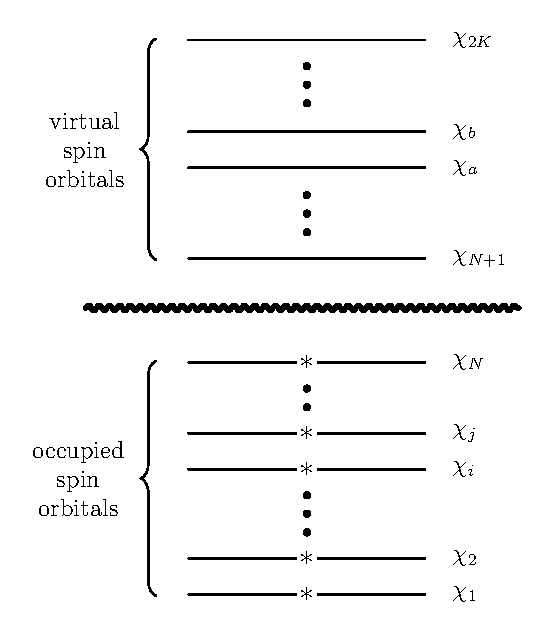
\includegraphics[width=0.30\textwidth]{fig/HF_det}
	\end{center}
\end{frame}

\begin{frame}{Excited determinants}
	\begin{block}{Singly-excited determinants}	
		\begin{equation}
			\qq*{Electron in $\green{i}$ promoted in $\red{a}$:} 
			\ket{\Psi_{\green{i}}^{\red{a}}} 
			= \ket*{\chi_1 \ldots \chi_{\red{a}} \chi_{\green{j}} \ldots \chi_N}
			= \cre{\red{a}} \ani{\green{i}} \ket{\Psi_0}
		\end{equation}
	\end{block}
	\begin{block}{Doubly-excited determinants}	
		\begin{equation}
			\qq*{Electrons in $\green{i}$ and $\green{j}$ promoted in $\red{a}$ and $\red{b}$:} 
			\ket*{\Psi_{\green{ij}}^{\red{ab}}} 
			= \ket{\chi_1 \ldots \chi_{\red{a}} \chi_{\red{b}} \ldots \chi_N}
			= \cre{\red{a}} \cre{\red{b}} \ani{\green{j}} \ani{\green{i}} \ket{\Psi_0}
		\end{equation}
	\end{block}
	\begin{center}
		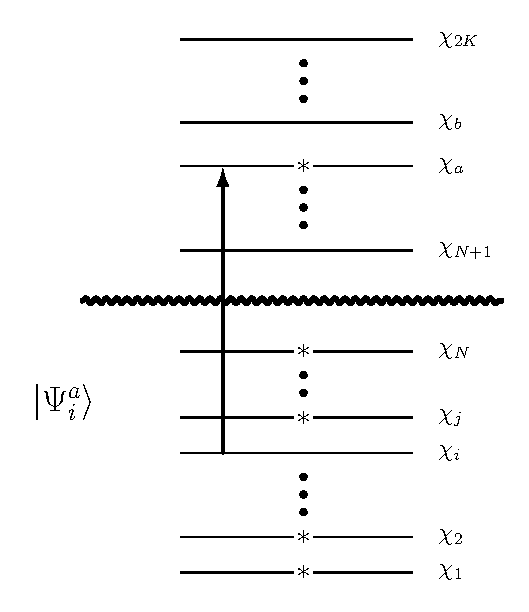
\includegraphics[width=0.22\textwidth]{fig/single}
		\hspace{0.2\textwidth}
		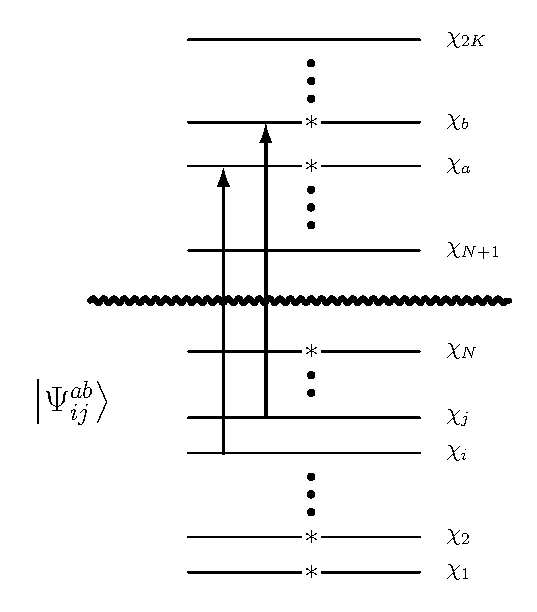
\includegraphics[width=0.22\textwidth]{fig/double}
	\end{center}
\end{frame}


%-----------------------------------------------------
\subsection{Slater-Condon}
%-----------------------------------------------------
\begin{frame}{Slater-Condon rules: One-electron operators}
	\small
	\begin{equation}
		\boxed{\chO_1 = \sum_i^N \hh(\br_i)}
	\end{equation}
	\begin{block}{Case 1: determinants differ by zero spin orbitals}
		\begin{equation}
			\qq*{$\ket{\red{K}} = \ket{\cdots i j \cdots} \quad \Rightarrow$} 
			\mel{\red{K}}{\chO_1}{\red{K}} = \sum_i^N \mel{i}{\hh}{i}
			\qq{\orange{Example:}}
			\mel*{\Psi_0}{\chO_1}{\Psi_0} = \sum_i^N h_{ii}
		\end{equation}
	\end{block}
	\begin{block}{Case 2: determinants differ by one spin orbital}
		\begin{equation}
			\qq*{$\ket{\red{K}} = \ket{\cdots i j \cdots}$ and $\ket{\blue{L}} = \ket{\cdots k j \cdots} \quad \Rightarrow$}	
			\mel{\red{K}}{\chO_1}{\blue{L}} = \mel{i}{\hh}{k}
			\qq{\orange{Example:}}
			\mel*{\Psi_0}{\chO_1}{\Psi_{\green{i}}^{\red{a}}} = h_{\green{i}\red{a}}
		\end{equation}
	\end{block}
	\begin{block}{Case 3: determinants differ by two spin orbitals}
		\begin{equation}
			\qq*{$\ket{\red{K}} = \ket{\cdots i j \ldots}$ and $\ket{\blue{L}} = \ket{\cdots k l \ldots} \quad \Rightarrow$}
			\mel{\red{K}}{\chO_1}{\blue{L}} = 0
			\qq{\orange{Example:}}
			\mel*{\Psi_0}{\chO_1}{\Psi_{\green{ij}}^{\red{ab}}} = 0
		\end{equation}
	\end{block}
\end{frame}

\begin{frame}{Slater-Condon rules: Two-electron operators}
	\small
	\begin{equation}
		\boxed{\chO_2 = \sum_{i<j}^N r_{ij}^{-1}}
	\end{equation}
	\begin{block}{Case 1: determinants differ by zero spin orbitals}
		\begin{equation}
			\qq*{$\ket{\red{K}} = \ket{\cdots i j \cdots} \quad \Rightarrow$}	
			\mel{\red{K}}{\chO_2}{\red{K}} = \frac{1}{2} \sum_{ij}^N \mel{ij}{}{ij}
			\qq{\orange{Example:}}
			\mel*{\Psi_0}{\chO_2}{\Psi_0} = \frac{1}{2} \sum_{ij}^N \mel{ij}{}{ij}
		\end{equation}
	\end{block}
	\begin{block}{Case 2: determinants differ by one spin orbital}
		\begin{equation}
			\qq*{$\ket{\red{K}} = \ket{\cdots i j \cdots}$ and $\ket{\blue{L}} = \ket{\cdots k j \cdots} \quad \Rightarrow$}	
			\mel{\red{K}}{\chO_2}{\blue{L}} = \sum_j^N \mel{ij}{}{kj}
			\qq{\orange{Example:}}
			\mel*{\Psi_0}{\chO_2}{\Psi_{\green{i}}^{\red{a}}} = \sum_k^N \mel{\green{i}k}{}{\red{a}k}
		\end{equation}
	\end{block}
	\begin{block}{Case 3: determinants differ by two spin orbitals}
		\begin{equation}
			\qq*{$\ket{\red{K}} = \ket{\cdots i j \cdots}$ and $\ket{\blue{L}} = \ket{\cdots k l \cdots} \quad \Rightarrow$}	
			\mel{\red{K}}{\chO_2}{\blue{L}} = \mel{ij}{}{kl}
			\qq{\orange{Example:}}
			\mel*{\Psi_0}{\chO_2}{\Psi_{\green{ij}}^{\red{ab}}} = \mel{\green{ij}}{}{\red{ab}}
		\end{equation}
	\end{block}
\end{frame}



%-----------------------------------------------------

\begin{frame}{Excited determinant vs excited HF solution}
	\begin{columns}[T,onlytextwidth]
		\begin{column}{0.48\textwidth}
			\begin{block}{What it is}
				\begin{itemize}
					\item An orbital substitution within a
					      \alert{fixed} set of reference orbitals
					\item A valid many-electron basis function
					\item A building block for CI and coupled-cluster
					      expansions
				\end{itemize}
			\end{block}
		\end{column}

		\begin{column}{0.48\textwidth}
			\begin{block}{What it is generally not}
				\begin{itemize}
					\item A separately optimized HF state
					\item A stationary point of the HF energy
					\item An eigenfunction of $\chS^2$
				\end{itemize}
			\end{block}
		\end{column}
	\end{columns}

	\begin{block}{Brillouin's theorem}
		For a stationary HF reference, the Hamiltonian does not couple
		the reference determinant to a singly-excited determinant:
		\begin{equation}
			\boxed{
				\mel{\Psi_0}{\chH_\text{elec}}{\Psi_i^a}
				=
				h_{ia} + \sum_j \mel{ij}{}{aj}
				=
				f_{ia}
				=
				0
			}
		\end{equation}
	\end{block}

	\centering
	\vfill
	$\Rightarrow$ \alert{Orbital excitation and state optimization are different procedures}
\end{frame}

%-----------------------------------------------------

\begin{frame}{A spin-free Hamiltonian conserves $S$ and $M_S$}
	\begin{block}{Spin operators}
    	In the nonrelativistic, spin-free framework, $\chH$ commutes with the spin operators
    	\begin{equation}
    		\boxed{
    			\comm{\chH}{\chS^2}=0
    			\qquad\text{and}\qquad
    			\comm{\chH}{\chS_z}=0
    		}
    	\end{equation}
    
    	The eigenfunctions of $\chH$ may therefore be chosen as simultaneous
    	eigenfunctions of $\chS^2$ and $\chS_z$:
    	\begin{align}
    		\chS^2\ket{S,M_S}
    		&=
    		S(S+1)\ket{S,M_S}
    		& 
    		\chS_z\ket{S,M_S}
    		&=
    		M_S\ket{S,M_S}
    	\end{align}
	\end{block}

	\begin{block}{Spin quantum numbers}
		\begin{itemize}
			\item $S$ determines the spin multiplicity $2S+1$
			\item $M_S=-S,-S+1,\ldots,S-1,S$ is its spin projection
		\end{itemize}
	\end{block}
\end{frame}

%-----------------------------------------------------

\begin{frame}{A determinant always has $M_S$, but not necessarily $S$}
	For a \alert{collinear} determinant containing $N^\alpha$ spin-up and
	$N^\beta$ spin-down orbitals:
	\begin{equation}
		\boxed{
			\chS_z\ket{\Phi}
			=
			M_S\ket{\Phi}
			\qquad
			M_S=\frac{N^\alpha-N^\beta}{2}
		}
	\end{equation}

	\begin{columns}[T,onlytextwidth]
		\begin{column}{0.48\textwidth}
			\begin{block}{Closed-shell RHF}
				Every spatial orbital is doubly occupied:
				\begin{equation}
					\chS^2\ket{\Phi_{\text{RHF}}}
					=
					0
				\end{equation}
				The determinant is a \alert{pure singlet}
			\end{block}
		\end{column}

		\begin{column}{0.48\textwidth}
			\begin{block}{Open-shell UHF}
				The alpha and beta spatial orbitals are different:
				\begin{equation}
					\chS^2\ket{\Phi_{\text{UHF}}}
					\neq
					S(S+1)\ket{\Phi_{\text{UHF}}}
				\end{equation}
				in general
			\end{block}
		\end{column}
	\end{columns}
	\vfill
	$\Rightarrow$
	\alert{Every RHF or UHF determinant has a well-defined $M_S$,
	but only specific determinants have a well-defined $S$}
\end{frame}

%-----------------------------------------------------

\begin{frame}{Spin contamination measures broken spin symmetry in UHF}
	\small
	For $N^\alpha \geq N^\beta$, a UHF determinant satisfies
	\begin{equation}
		\boxed{
			\expval{\chS^2}_{\text{UHF}}
			=
			M_S(M_S+1)
			+
			N^\beta
			-
			\sum_{i=1}^{N^\alpha}
			\sum_{j=1}^{N^\beta}
			\abs{S_{ij}^{\alpha\beta}}^2
		}
	\end{equation}
	with
	\begin{equation}
		\underbrace{S_{ij}^{\alpha\beta}}_{\text{overlap}}
		=
		\braket{\phi_i^\alpha}{\phi_j^\beta}
		\qq{and}
		M_S=\frac{N^\alpha-N^\beta}{2}
	\end{equation}

	\begin{block}{Spin contamination}
		For a high-spin target state with $S=M_S$,
		\begin{equation}
			\Delta S^2
			=
			\expval{\chS^2}_{\text{UHF}}
			-
			S(S+1)
			\geq 0
		\end{equation}

    	\begin{itemize}
    		\item A singlet may be contaminated by triplets, quintets, \ldots 
    		\item A doublet may be contaminated by quartets, sextets, \ldots 
    		\item A triplet may be contaminated by quintets, septets, \ldots 
    		\item Restoring spin symmetry generally requires \alert{spin projection} or \alert{a linear combination of determinants}
    	\end{itemize}
	\end{block}
\end{frame}

%-----------------------------------------------------
\begin{frame}{A singly excited determinant is not necessarily spin adapted}
	Start from a closed-shell singlet reference and define the determinant phases by
	\begin{equation}
		\ket{D_\alpha}
		=
		\cre{a\alpha}\ani{i\alpha}\ket{\Psi_0},
		\qquad
		\ket{D_\beta}
		=
		\cre{a\beta}\ani{i\beta}\ket{\Psi_0}.
	\end{equation}

	\begin{columns}[T,onlytextwidth]
		\begin{column}{0.46\textwidth}
			\begin{block}{$\ket*{D_\alpha}$: excite the $\alpha$ electron}
				\centering
				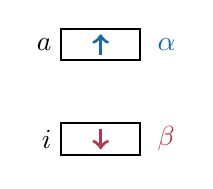
\begin{tikzpicture}[x=1cm,y=1cm]
					\node[left] at (0,0.35) {$i$};
					\node[left] at (0,1.55) {$a$};
					\draw[thick] (0,0.15) rectangle (1.0,0.55);
					\draw[thick] (0,1.35) rectangle (1.0,1.75);
					\draw[hfRed,very thick,->] (0.50,0.48)--(0.50,0.22);
					\draw[hfBlue,very thick,->] (0.50,1.42)--(0.50,1.68);
					\node[hfRed,right] at (1.10,0.35) {$\beta$};
					\node[hfBlue,right] at (1.10,1.55) {$\alpha$};
				\end{tikzpicture}
			\end{block}
		\end{column}
		\begin{column}{0.46\textwidth}
			\begin{block}{$\ket*{D_\beta}$: excite the $\beta$ electron}
				\centering
				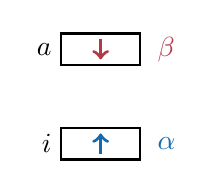
\begin{tikzpicture}[x=1cm,y=1cm]
					\node[left] at (0,0.35) {$i$};
					\node[left] at (0,1.55) {$a$};
					\draw[thick] (0,0.15) rectangle (1.0,0.55);
					\draw[thick] (0,1.35) rectangle (1.0,1.75);
					\draw[hfBlue,very thick,->] (0.50,0.22)--(0.50,0.48);
					\draw[hfRed,very thick,->] (0.50,1.68)--(0.50,1.42);
					\node[hfBlue,right] at (1.10,0.35) {$\alpha$};
					\node[hfRed,right] at (1.10,1.55) {$\beta$};
				\end{tikzpicture}
			\end{block}
		\end{column}
	\end{columns}

	\begin{align}
		\chS_z\ket{D_\sigma}&=0,
		&
		\mel{D_\sigma}{\chS^2}{D_\sigma}&=1.
	\end{align}

	\begin{block}{Same $M_S$, indefinite total spin}
		Each determinant has $M_S=0$, but contains equal singlet and triplet character.
		Being an eigenfunction of $\chS_z$ does not imply being an eigenfunction of $\chS^2$.
	\end{block}
\end{frame}

%-----------------------------------------------------
\begin{frame}{Diagonalizing $\chS^2$ produces pure singlet and triplet states}
	In the two-determinant basis $\{\ket{D_\alpha},\ket{D_\beta}\}$,
	\begin{equation}
		\boxed{
			\left[\chS^2\right]_{\{D_\alpha,D_\beta\}}
			=
			\begin{pmatrix}
				 1 & -1 \\
				-1 &  1
			\end{pmatrix}
		}
		\qquad (\hbar=1).
	\end{equation}

	\begin{columns}[T,onlytextwidth]
		\begin{column}{0.48\textwidth}
			\begin{block}{Pure singlet}
				\begin{equation}
					\boxed{
						\ket{{}^1\Phi_i^a}
						=
						\frac{1}{\sqrt2}
						\left(
							\ket{D_\alpha}+\ket{D_\beta}
						\right)
					}
				\end{equation}
				\begin{equation}
					\chS^2\ket{{}^1\Phi_i^a}=0,
					\qquad S=0.
				\end{equation}
			\end{block}
		\end{column}
		\begin{column}{0.48\textwidth}
			\begin{block}{Pure triplet, $M_S=0$}
				\begin{equation}
					\boxed{
						\ket{{}^3\Phi_i^a;0}
						=
						\frac{1}{\sqrt2}
						\left(
							\ket{D_\alpha}-\ket{D_\beta}
						\right)
					}
				\end{equation}
				\begin{equation}
					\chS^2\ket{{}^3\Phi_i^a;0}
					=
					2\ket{{}^3\Phi_i^a;0},
					\qquad S=1.
				\end{equation}
			\end{block}
		\end{column}
	\end{columns}

	\begin{equation}
		\boxed{
			\text{spin adaptation}
			=
			\text{diagonalization of $\chS^2$ in a determinant space}
		}
	\end{equation}

	\centering
	\scriptsize
	The relative $+$ and $-$ signs depend on determinant phases; the excitation-operator
	definitions on the preceding slide fix the convention used here.
\end{frame}

%-----------------------------------------------------
\begin{frame}{Spin and spatial symmetry compensate each other}
	For the two open-shell spatial orbitals $i$ and $a$, the singlet is
	\begin{equation}
		\Psi_{ia}^{S=0}
		=
		\frac{1}{2}
		\underbrace{
			\left[
				\phi_i(1)\phi_a(2)+\phi_a(1)\phi_i(2)
			\right]
		}_{\text{spatially symmetric}}
		\underbrace{
			\left[
				\alpha(1)\beta(2)-\beta(1)\alpha(2)
			\right]
		}_{\text{spin antisymmetric}}.
	\end{equation}

	\begin{block}{Singlet: opposite exchange symmetries}
		\centering
		\green{symmetric spatial part}
		$\times$
		\red{antisymmetric spin part}
	\end{block}

	The $M_S=0$ triplet is
	\begin{equation}
		\Psi_{ia}^{S=1,M_S=0}
		=
		\frac{1}{2}
		\underbrace{
			\left[
				\phi_i(1)\phi_a(2)-\phi_a(1)\phi_i(2)
			\right]
		}_{\text{spatially antisymmetric}}
		\underbrace{
			\left[
				\alpha(1)\beta(2)+\beta(1)\alpha(2)
			\right]
		}_{\text{spin symmetric}}.
	\end{equation}

	\begin{block}{Triplet: opposite exchange symmetries}
		\centering
		\red{antisymmetric spatial part}
		$\times$
		\green{symmetric spin part}
	\end{block}

	\centering
	\boxed{
		\text{The complete electronic wave function is antisymmetric in both cases.}
	}
\end{frame}

%-----------------------------------------------------
\begin{frame}{The $M_S=0$ combination belongs to a three-component triplet}
	The three components of the $S=1$ multiplet are
	\begin{equation}
		\boxed{
		\begin{aligned}
			\ket{{}^3\Phi_i^a;+1}
				&=\ket{\cdots i^\alpha a^\alpha\cdots},\\[1mm]
			\ket{{}^3\Phi_i^a;0}
				&=\frac{1}{\sqrt2}
				\left(\ket{D_\alpha}-\ket{D_\beta}\right),\\[1mm]
			\ket{{}^3\Phi_i^a;-1}
				&=\ket{\cdots i^\beta a^\beta\cdots}.
		\end{aligned}}
	\end{equation}

	Every component satisfies
	\begin{equation}
		\chS^2\ket{1,M_S}=2\ket{1,M_S},
		\qquad
		\chS_z\ket{1,M_S}=M_S\ket{1,M_S}.
	\end{equation}

	They are connected by
	\begin{equation}
		\chS_\pm\ket{S,M_S}
		=
		\sqrt{S(S+1)-M_S(M_S\pm1)}
		\ket{S,M_S\pm1}.
	\end{equation}

	\begin{columns}[T,onlytextwidth]
		\begin{column}{0.48\textwidth}
			\begin{block}{$M_S=\pm1$}
				Each component is a single spin-pure determinant.
			\end{block}
		\end{column}
		\begin{column}{0.48\textwidth}
			\begin{block}{$M_S=0$}
				The pure triplet requires a two-determinant combination.
			\end{block}
		\end{column}
	\end{columns}

	\centering
	\alert{The open-shell singlet likewise requires two determinants.}
\end{frame}

%-----------------------------------------------------
\subsection{Examples}
%-----------------------------------------------------
\begin{frame}{Normalization of a two-electron determinant}
	\begin{block}{Problem: Normalization of the HF wave function}
		\textit{\violet{``Show that the HF wave function built with two (normalized) spin orbitals $\chi_1$ and $\chi_2$ is normalized''}}
	\end{block}
	\pause
	\begin{block}{Solution}
		\small
		\begin{equation*}
			\Psi_\text{HF} = 
			\frac{1}{\sqrt{2}}
			\begin{vmatrix}
				\chi_1(1)	&	\chi_2(1)		\\
				\chi_1(2)	&	\chi_2(2)		\\
			\end{vmatrix}
			= \frac{ \chi_1(1) \chi_2(2) -  \chi_1(2) \chi_2(1)}{\sqrt{2}}
		\end{equation*}
		\begin{equation*}
		\begin{split}
			\braket{\Psi_\text{HF}}{\Psi_\text{HF}} 
			& = \frac{1}{2} \braket{\chi_1(1) \chi_2(2) -  \chi_2(1) \chi_1(2)}{ \chi_1(1) \chi_2(2) -  \chi_2(1) \chi_1(2) }
			\\
			& = \frac{1}{2} \Big[ 
			\braket{ \chi_1(1) \chi_2(2)  }{ \chi_1(1) \chi_2(2)  }
			- \braket{ \chi_1(1) \chi_2(2)  }{   \chi_2(1) \chi_1(2) }
			\\
			& - \braket{ \chi_2(1) \chi_1(2) }{ \chi_1(1) \chi_2(2)  }
			+ \braket{ \chi_2(1) \chi_1(2) }{   \chi_2(1) \chi_1(2) }
			\Big]
			\\
			& =  \frac{1}{2} \Big[ 1 - 0 - 0 + 1 \Big] = 1
		\end{split}
		\end{equation*}
		\alert{Remember that $\braket{\chi_1(1) \chi_2(2) }{ \chi_1(1) \chi_2(2)  } = \braket{ \chi_1(1)   }{ \chi_1(1)  } \braket{ \chi_2(2)  }{ \chi_2(2)  }$}
	\end{block}
\end{frame}

\begin{frame}{One-electron energy of a two-electron determinant}
	\begin{block}{Problem: Core Hamiltonian}
		\textit{\violet{``Show that $ \mel{\Psi_\text{HF}}{\chO_1}{\Psi_\text{HF}}  = \sum_{i=1}^N h_{ii}  $ for the same system''}}
	\end{block}
	\pause
	\begin{block}{Solution}
		\small
		\begin{equation*}
			\chO_1 = \hh(1) + \hh(2)
		\end{equation*}
		\begin{equation*}
		\begin{split}
			& \mel{ \Psi_\text{HF} }{ \hh(1) + \hh(2) }{ \Psi_\text{HF} } 
			\\
			& \qquad = \frac{1}{2} \mel{ \chi_1(1) \chi_2(2) -  \chi_1(2) \chi_2(1) }{ \hh(1) + \hh(2) }{ \chi_1(1) \chi_2(2) -  \chi_1(2) \chi_2(1) }
			\\
			&  \qquad = \frac{1}{2} \Big[ 
			\mel{ \chi_1(1) \chi_2(2) }{ \hh(1) + \hh(2) }{ \chi_1(1) \chi_2(2) }
			- \mel{ \chi_1(1) \chi_2(2) }{ \hh(1) + \hh(2) }{ \chi_2(1) \chi_1(2) }
			\\
			&  \qquad - \mel{  \chi_2(1) \chi_1(2) }{ \hh(1) + \hh(2) }{ \chi_1(1) \chi_2(2)  }
			+ \mel{  \chi_2(1) \chi_1(2) }{ \hh(1) + \hh(2) }{  \chi_2(1) \chi_1(2) }
			\Big]
			\\
			&  \qquad =  \frac{1}{2} \Big[ h_{11} + h_{22} - 0 - 0 + h_{22} + h_{11} \Big] = h_{11} + h_{22}
		\end{split}
		\end{equation*}
	\end{block}
\end{frame}

\begin{frame}{Electron interaction in a two-electron determinant}
	\begin{block}{Problem: Two-electron Hamiltonian}
		\textit{\violet{``Show that $ \mel{\Psi_\text{HF}}{\chO_2}{\Psi_\text{HF}}  =  \sum_{i<j}^N \qty( \cJ_{ij} - \cK_{ij} )$ for the same system and write down the HF energy''}}
	\end{block}
	\pause
	\begin{block}{Solution}
		\small
		\begin{equation*}
			\chO_2 =r_{12}^{-1}
		\end{equation*}
		\begin{equation*}
		\begin{split}
			\mel{ \Psi_\text{HF} }{ r_{12}^{-1} }{ \Psi_\text{HF} } 
			&  = \frac{1}{2} \mel{ \chi_1 \chi_2 -  \chi_2 \chi_1 }{ r_{12}^{-1} }{ \chi_1 \chi_2 -  \chi_2 \chi_1 }
			\\
			&   = \frac{1}{2} \Big[ 
			\mel{ \chi_1 \chi_2 }{ r_{12}^{-1} }{ \chi_1 \chi_2 }
			- \mel{ \chi_1 \chi_2 }{ r_{12}^{-1} }{  \chi_2 \chi_1 }
			\\
			&   - \mel{  \chi_2 \chi_1 }{ r_{12}^{-1} }{ \chi_1 \chi_2  }
			+ \mel{  \chi_2 \chi_1 }{ r_{12}^{-1} }{  \chi_2 \chi_1 }
			\Big]
			\\
			&   =  \frac{1}{2} \Big[ \cJ_{12} - \cK_{12} - \cK_{12} + \cJ_{12} \Big] = \cJ_{12} - \cK_{12}
		\end{split}
		\end{equation*}
		\alert{Remember that $\mel{  \chi_2 \chi_1 }{ r_{12}^{-1} }{  \chi_2 \chi_1 } = \mel{  \chi_1 \chi_2 }{ r_{12}^{-1} }{  \chi_1 \chi_2 }$}
		\begin{equation*}
			\boxed{E_\text{HF} = h_{11} + h_{22} + \cJ_{12} - \cK_{12}}
		\end{equation*}
	\end{block}
\end{frame}

\begin{frame}{HF energy of a three-electron system}
	\begin{block}{Three-electron system}
		\textit{\violet{``Find the HF energy of a three-electron system composed of the spin orbitals $\chi_1$, $\chi_2$ and $\chi_3$''}}
	\end{block}
	\pause
	\begin{block}{Solution}
		\begin{gather*}
			\chO_1 = \hh(\bx_1) + \hh(\bx_2) + \hh(\bx_3)
			\\
			\chO_2 =r_{12}^{-1} + r_{13}^{-1} + r_{23}^{-1}
		\end{gather*}
		$$ \vdots $$
		\begin{equation*}
			\boxed{E_\text{HF} = h_{11} + h_{22} + h_{33} + \cJ_{12} + \cJ_{13} + \cJ_{23} - \cK_{12} - \cK_{13} - \cK_{23}}
		\end{equation*}
	\end{block}
\end{frame}

%\begin{frame}{HF energy of \ce{He}}
%	\begin{columns}
%		\begin{column}{0.55\textwidth}
%			\begin{block}{Singlet $1s^2$ state of the \ce{He} atom}
%				$$ \chi_1 = \alpha \, \psi_1 \qquad \chi_2 = \beta \, \psi_1$$
%				\begin{equation*}
%					\orange{E_\text{HF}(\text{singlet})} = h_1 + h_2 + \cJ_{12} - \cK_{12} = \orange{2 h_1 + J_{11}}
%				\end{equation*}
%			\end{block}
%		\end{column}
%		\begin{column}{0.45\textwidth}
%			\begin{equation*}
%			\begin{split}
%				\cJ_{12} 
%				& = \langle \chi_1 \chi_2 | \chi_1 \chi_2 \rangle
%				\\
%				& = \langle \alpha | \alpha \rangle \langle \beta | \beta \rangle \langle \psi_1 \psi_1 | \psi_1 \psi_1 \rangle
%				= J_{11}
%			\end{split}
%			\end{equation*}
%			\begin{equation*}
%			\begin{split}
%				\cK_{12} 
%				& = \langle \chi_1 \chi_2 | \chi_2 \chi_1 \rangle
%				\\
%				& = \langle \alpha | \beta \rangle \langle \beta | \alpha \rangle \langle \psi_1 \psi_1 | \psi_1 \psi_1 \rangle
%				= 0
%			\end{split}
%			\end{equation*}
%		\end{column}
%	\end{columns}
%	\begin{block}{Triplet $1s2s$ state of the \ce{He} atom}
%		$$ \chi_1 = \alpha \, \psi_1 \qquad \chi_2 = \alpha \, \psi_2$$
%		\begin{equation*}
%			\alert{E_\text{HF}(\text{triplet})} = h_1 + h_2 + \cJ_{12} - \cK_{12} = \alert{h_1 + h_2 + J_{12} - K_{12}}
%		\end{equation*}
%	\end{block}
%	\begin{block}{Singlet-triplet energy splitting}
%		\begin{equation*}
%		\begin{split}
%			\Delta E_\text{HF} 
%			& = \alert{E_\text{HF}(\text{triplet})} - \orange{E_\text{HF}(\text{singlet})} 
%			\\
%			& = \underbrace{(\alert{h_2} - \orange{h_1})}_{>0} + \underbrace{(\alert{J_{12}} - \orange{J_{11}})}_{<0} - \alert{K_{12}}
%		\end{split}
%		\end{equation*}
%	\end{block}
%\end{frame}


%-----------------------------------------------------
\subsection{Spin to spatial}
%-----------------------------------------------------
\begin{frame}{Closed-shell \ce{H2} in spatial orbitals}
	\begin{columns}
		\begin{column}{0.6\textwidth}
			\begin{block}{Two-electron example: \ce{H2} in minimal basis}
				In the spin orbital basis, we have
				\begin{equation*}		
					\EHF 
					= \mel{\chi_1}{\hh}{\chi_1} + \mel{\chi_2}{\hh}{\chi_2} 
					+ \braket{\chi_1 \chi_2}{\chi_1 \chi_2} - \braket{\chi_1 \chi_2}{\chi_2 \chi_1}
				\end{equation*}
				Spin to spatial transformation:
				\begin{align*}
					\chi_1(\bx) & \equiv \psi_1(\bx) = \psi_1(\br) \alpha(\omega)
					\\
					\chi_2(\bx) & \equiv \Bar{\psi}_1(\bx) = \psi_1(\br) \beta(\omega)
				\end{align*}
				\begin{equation*}		
					\EHF 
					= \rmel{\psi_1 }{ \hh }{ \psi_1 } + \rmel{\Bar{\psi}_1 }{ \hh }{ \Bar{\psi}_1 } 
					+ \rbraket{ \psi_1 \psi_1 }{ \Bar{\psi}_1 \Bar{\psi}_1 } - \rbraket{ \psi_1 \Bar{\psi_1} }{ \Bar{\psi}_1 \psi_1 } 
				\end{equation*}
				Therefore, in the spatial orbital basis, we have
				\begin{equation*}		
					\EHF = 2\rmel{\psi_1}{\hh}{\psi_1} + \rbraket{\psi_1 \psi_1}{\psi_1 \psi_1} = 2\rmel{1}{\hh}{1} + \rbraket{11}{11}
				\end{equation*}
			\end{block}
		\end{column}
		\begin{column}{0.4\textwidth}
			\begin{center}
				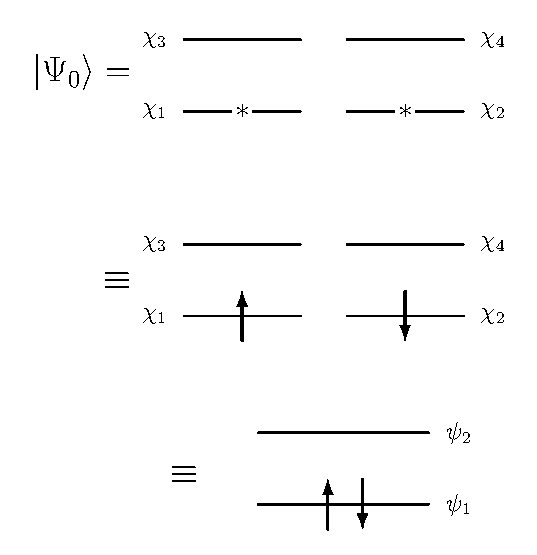
\includegraphics[width=\textwidth]{fig/H2}
			\end{center}
		\end{column}
	\end{columns}
\end{frame}

\begin{frame}{Integrating the one-electron spin coordinate}
	\small
	\begin{block}{One-electron terms}
		\begin{equation*}
		\begin{split}
			\rmel{\chi_1}{\hh}{\chi_1}
			& = \int \chi_1^*(\bx) \hh(\br) \chi_1(\bx) \dd{\bx} 
			\\
			& = \iint \alpha^*(\omega) \psi_1^*(\br) \hh(\br) \alpha(\omega) \psi_1(\br) \dd{\omega} \dd{\br} 
			\\
			& = \underbrace{\qty[ \int \alpha^*(\omega) \alpha(\omega) \dd{\omega} ]}_{=1} 
			\underbrace{\qty[ \int \psi_1^*(\br) \hh(\br) \psi_1(\br) \dd{\br}]}_{\rmel{\psi_1}{\hh}{\psi_1}  }
		\end{split}
		\end{equation*}
		\begin{equation*}
		\begin{split}
			\rmel{\chi_2}{\hh}{\chi_2} 
			& = \int \chi_2^*(\bx) \hh(\br) \chi_2(\bx) \dd{\bx} 
			\\
			& = \iint \beta^*(\omega) \psi_1^*(\br) \hh(\br) \beta(\omega) \psi_1(\br) \dd{\omega} \dd{\br} 
			\\
			& = \underbrace{\qty[ \int \beta^*(\omega) \beta(\omega) \dd{\omega} ]}_{=1} 
			\underbrace{\qty[ \int \psi_1^*(\br) \hh(\br) \psi_1(\br)  \dd{\br} ]}_{\rmel{\psi_1}{\hh}{\psi_1} }
		\end{split}
		\end{equation*}
	\end{block}
\end{frame}

\begin{frame}{Integrating spin in Coulomb and exchange terms}
	\begin{block}{Two-electron terms}
	\small
		\begin{equation*}
		\begin{split}
			\rbraket{\chi_1 \chi_1}{\chi_2 \chi_2}
			& = \iint \chi_1^*(\bx_1) \chi_1(\bx_1) r_{12}^{-1} \chi_2^*(\bx_2) \chi_2(\bx_2) \dd{\bx_1} \dd{\bx_2} 
			\\
			& = \iint \iint \alpha^*(\omega_1) \psi_1^*(\br_1) \alpha(\omega_1) \psi_1(\br_1) r_{12}^{-1} \beta^*(\omega_2) \psi_1^*(\br_2) \beta(\omega_2) \psi_1(\br_2) \dd{\omega_1} \dd{\br_1} \dd{\omega_2} \dd{\br_2} 
			\\
			& = \underbrace{\qty[ \int \alpha^*(\omega_1) \alpha(\omega_1) \dd{\omega_1} ]}_{=1} 
			\underbrace{\qty[ \int \beta^*(\omega_2) \beta(\omega_2) \dd{\omega_2} ]}_{=1} 
			\underbrace{\qty[ \iint \psi_1^*(\br_1) \psi_1(\br_1) r_{12}^{-1} \psi_1^*(\br_2) \psi_1(\br_2) \dd{\br_1} \dd{\br_2} ]}_{\rbraket{\psi_1 \psi_1}{\psi_1 \psi_1}}
		\end{split}
		\end{equation*}
		\begin{equation*}
		\begin{split}
			\rbraket{\chi_1 \chi_2}{\chi_2 \chi_1}
			& = \iint \chi_1^*(\bx_1) \chi_2(\bx_1) r_{12}^{-1} \chi_2^*(\bx_2) \chi_1(\bx_2) \dd{\bx_1} \dd{\bx_2} 
			\\
			& = \iint \iint \alpha^*(\omega_1) \psi_1^*(\br_1) \beta(\omega_1) \psi_1(\br_1) r_{12}^{-1} \beta^*(\omega_2) \psi_1^*(\br_2) \alpha(\omega_2) \psi_1(\br_2) \dd{\omega_1} \dd{\br_1} \dd{\omega_2} \dd{\br_2} 
			\\
			& = \underbrace{\qty[ \int \alpha^*(\omega_1) \beta(\omega_1) \dd{\omega_1} ]}_{=0} 
			\underbrace{\qty[ \int \beta^*(\omega_2) \alpha(\omega_2) \dd{\omega_2} ]}_{=0} 
			\underbrace{\qty[ \iint \psi_1^*(\br_1) \psi_1(\br_1) r_{12}^{-1} \psi_1^*(\br_2) \psi_1(\br_2) \dd{\br_1} \dd{\br_2} ]}_{\rbraket{\psi_1 \psi_1}{\psi_1 \psi_1}}
		\end{split}
		\end{equation*}
	\end{block}
\end{frame}



\begin{frame}{Closed-shell Hartree-Fock energy in spatial orbitals}
	\begin{block}{General expression}
		\begin{equation}
			\EHF 
			= \sum_i^N \mel{i}{\hh}{i} + \frac{1}{2} \sum_i^N \sum_j^N \qty[ \braket{ij}{ij} - \braket{ij}{ji} ]
			= 2 \sum_i^{N/2} \rmel{i}{\hh}{i} + \sum_i^{N/2} \sum_j^{N/2} \qty[ 2\rbraket{ii}{jj} - \rbraket{ij}{ji} ]
		\end{equation}
	\end{block}
	\begin{block}{One- and two-electron terms}
		\small
		\begin{equation}
			\sum_i^N \mel{i}{\hh}{i} = \sum_i^{N/2} \mel{i}{\hh}{i} + \sum_a^{N/2} \mel{\Bar{i}}{\hh}{\Bar{i}} = 2 \sum_i^{N/2} \rmel{i}{\hh}{i}
		\end{equation}
		\begin{equation}
		\begin{split}
			\frac{1}{2} \sum_i^N \sum_j^N \qty[ \braket{ij}{ij} - \braket{ij}{ji} ]
			& = \frac{1}{2} \Bigg\{  
				  \sum_i^{N/2} \sum_j^{N/2} \qty( \braket{ij}{ij} - \braket{ij}{ji} )
				+ \sum_i^{N/2} \sum_j^{N/2} \qty( \braket{\Bar{i}j}{\Bar{i}j} - \braket{\Bar{i}j}{j\Bar{i}} )
				\\
				& \qquad + \sum_i^{N/2}  \sum_j^{N/2} \qty( \braket{i\Bar{j}}{i\Bar{j}} - \braket{i\Bar{j}}{\Bar{j}i} )
				+ \sum_i^{N/2}  \sum_j^{N/2} \qty( \braket{\Bar{i}\Bar{j}}{\Bar{i}\Bar{j}} - \braket{\Bar{i}\Bar{j}}{\Bar{j}\Bar{i}} )
				\Bigg\}
			\\
			& = \sum_i^{N/2} \sum_j^{N/2} \qty[ 2\rbraket{ii}{jj} - \rbraket{ij}{ji} ]
		\end{split}
		\end{equation}
	\end{block}	
\end{frame}


\begin{frame}{Hartree-Fock energy of atoms}
	\begin{block}{Problem: HF energy of the \ce{Li} atom}
		\violet{``Find the HF energy of the \ce{Li} atom in terms of spatial orbitals''}
	\end{block}
	\pause
	\begin{block}{Solution}
		$$ \chi_1 = \alpha \psi_1 \qquad \chi_2 = \beta \psi_1
		\qquad \chi_3 = \alpha \psi_2 $$
		\begin{equation*}
			E_\text{HF} = 2 h_{11} + h_{22} + J_{11} + 2J_{12} - K_{12}
		\end{equation*}
	\end{block}
	\pause
	\begin{block}{Problem: HF energy of the \ce{B} atom}
		\violet{``Find the HF energy of the \ce{B} atom in terms of spatial orbitals''}
	\end{block}
	\pause
	\begin{block}{Solution}
		$$ E_\text{HF} = 2h_{11} + 2h_{22} + h_{33} + J_{11} + 4J_{12} + J_{22} - 2K_{12} + 2J_{13} + 2J_{23} - K_{13} - K_{23}$$
	\end{block}
\end{frame}

%-----------------------------------------------------
\subsection{Fock matrix}
%-----------------------------------------------------
\begin{frame}{The Fock matrix}
	The \alert{stationarity of the HF energy} wrt the spin orbitals implies that 
	\begin{equation}
		\fdv{E_\text{HF}}{\chi_i} = 0
		\qq{$\Rightarrow$}
		\boxed{\hf(\bx_1) \chi_i(\bx_1) = \underbrace{\epsilon_i}_{\alert{\text{orbital energies}}} \chi_i(\bx_1)}
	\end{equation}	
	where $\hf$ is the \alert{one-electron Fock operator}
	\begin{equation}
		\boxed{ \hf(\bx_1) = \hh(\bx_1) + \underbrace{\sum_i^N [\chJ_i(\bx_1) - \chK_i(\bx_1)]}_{\Hat{v}^\text{HF}(\bx_1) \text{ = \alert{Hartree-Fock potential}}}}
	\end{equation}	
	For a \alert{closed-shell system} (i.e., two electrons in each spatial orbital)
	 \begin{equation*}
		\hf(\br_1) = \hh(\br_1) + \sum_i^{N/2} \qty[2 \hJ_i(\br_1) - \hK_i(\br_1)]	\quad \text{\alert{(closed shell)}}	
	\end{equation*}	
\end{frame}

\begin{frame}{Fock matrix elements in the spin orbital basis}
	\begin{block}{Problem:}
		\violet{`` Find the expression of the matrix elements $f_{ij} = \mel{\chi_i}{\hf}{\chi_j}$''}
	\end{block}
	\pause
	\begin{block}{Solution}
		\begin{equation*}
		\begin{split}
			\mel{\chi_i}{\hf}{\chi_j} 
			& = \mel{\chi_i}{\hh + \sum_k \qty( \chJ_k - \chK_k)}{\chi_j}
			\\
			& = \mel{\chi_i}{\hh}{\chi_j} + \sum_k \qty( \mel{\chi_i}{\chJ_k}{\chi_j} - \mel{\chi_i}{\chK_k}{\chi_j} )
			\\
			& = \mel{i}{\hh}{j} + \sum_k \qty[ \braket{ik}{jk} - \braket{ik}{kj} ]
			\\
			& = \mel{i}{\hh}{j} + \sum_k \mel{ik}{}{jk}
		\end{split}
		\end{equation*}
	\end{block}
\end{frame}

\begin{frame}{Orbital energies in the spin orbital basis}
	\begin{block}{Problem:}
		\violet{`` Deduce the expression of $\epsilon_i$''}
	\end{block}
	\pause
	\begin{block}{Solution}
		\begin{align*}
			\hf \ket{\chi_i} = \epsilon_i \ket{\chi_i}
			& \Rightarrow \quad \mel{\chi_i}{\hf}{\chi_i} = \epsilon_i \braket{\chi_i}{\chi_i} = \epsilon_i
			\\
			& \Rightarrow \quad \epsilon_i = \mel{i}{\hh}{i} + \sum_k \qty[ \braket{ik}{ik} - \braket{ik}{ki} ]
			\\
			& \Rightarrow \quad \epsilon_i = \mel{i}{\hh}{i} + \sum_k \mel{ik}{}{ik}
		\end{align*}
	\end{block}
\end{frame}

%%-----------------------------------------------------
%\subsection{Variational principle}
%%-----------------------------------------------------
%\begin{frame}{The variational principle}
%	\begin{block}{Problem}
%		\violet{\textit{``Let's suppose we know all the functions such as $\hH \varphi_i = E_i \varphi_i$, with $E_0 < E_1 < \ldots $ and $\braket{ \varphi_i }{ \varphi_j } = \delta_{ij}$.
%		Show that, for any normalized $\Psi$, we have $ E = \mel{ \Psi }{ \hH }{ \Psi } \ge E_0$''}}
%		\pause
%	\end{block}
%	\begin{block}{Solution}
%		We expand $\Psi$ in a \alert{clever basis} 
%		\begin{equation*}
%			\Psi = \sum_{i}^\infty c_i \,\varphi_i 
%			\qq{with}
%			\sum_{i}^\infty c_i^2 = 1
%		\end{equation*}
%		\pause
%		\begin{equation*}
%		\begin{split}
%			E 	& = \mel{ \Psi }{ \hH }{ \Psi } 	
%				= \mel{ \sum_i c_i \varphi_i }{ \hH }{ \sum_j c_j \varphi_j } 
%				= \sum_{ij} c_i c_j \mel{ \varphi_i }{ \hH }{ \varphi_j } 
%			\\
%				& = \sum_{ij} c_i c_j E_j \braket{ \varphi_i }{ \varphi_j } 
%				= \sum_{ij} c_i c_j E_j \delta_{ij} 
%				= \sum_{i} c_i^2 E_i  \ge E_0  \sum_{i} c_i^2 = E_0
%		\end{split}
%		\end{equation*}
%	\end{block}
%\end{frame}

%-----------------------------------------------------
\subsection{Koopmans}
%-----------------------------------------------------
\begin{frame}{Koopmans' theorem}
	\small
	\begin{block}{Ground-state energy of the $N$-electron system}
		\begin{equation}
			{}^{N} E_0  = \sum_{i} h_{ii} + \frac{1}{2} \sum_{ij} \mel{ij}{}{ij}
		\end{equation}
	\end{block}
	\begin{block}{Energy of the $(N-1)$-electron system (cation)}
		\begin{equation}
			{}^{N-1}E_k  = \sum_{i \neq k} h_{ii} + \frac{1}{2} \sum_{i \neq k} \sum_{j \neq k} \mel{ij}{}{ij}
		\end{equation}
	\end{block}
	\begin{block}{Ionization potential (IP)}
		\begin{equation}
		\begin{split}
			\text{IP} 
			& = {}^{N-1}E_k - {}^{N} E_0
			\\
			& = - \mel{k}{\hh}{k} - \frac{1}{2} \sum_{i} \mel{ik}{}{ik} - \frac{1}{2} \sum_{j} \mel{kj}{}{kj}
			\\
			& = - \mel{k}{\hh}{k} - \sum_{i} \mel{ik}{}{ik} 
			= - \epsilon_k 
		\end{split}
		\end{equation}
	\end{block}
\end{frame}

\begin{frame}{Koopmans' theorem for electron affinity (EA)}
	\begin{block}{Problem:}
		\violet{``Show that Koopmans' theorem applies to electron affinities''}
	\end{block}
	\pause
	\begin{block}{Solution}
		\begin{equation}
		\begin{split}
			\text{EA} 
			& = {}^{N}E_0 - {}^{N+1} E^c
			\\
			& = - \mel{c}{\hh}{c} - \sum_{i} \mel{ci}{}{ci} 
			\\
			& = - \epsilon_c 
		\end{split}
		\end{equation}

	\end{block}
\end{frame}

\begin{frame}{Hartree-Fock Hamiltonian}
	\begin{block}{Definition}
		\begin{equation}
			\underbrace{\chH^\text{HF}}_{\text{\alert{$N$-electron} operator}} 
			= \sum_i^N \underbrace{\hf(\bx_i)}_{\text{\alert{one-electron} operator}}
			= \sum_i^N \qty[ \hh(\bx_i) + \Hat{v}^\text{HF}(\bx_i) ]
		\end{equation}
	\end{block}
	\begin{block}{Warnings!}
		\begin{equation}
			\chH^\text{HF} \ket{\Psi_\text{HF}} = \qty( \sum_i^N \epsilon_i ) \ket{\Psi_\text{HF}}
			\alert{\neq} E_\text{HF} \ket{\Psi_\text{HF}}
		\end{equation}
		The HF wavefunction is an eigenfunction of the HF Hamiltonian, but the eigenvalue is \alert{not} the HF energy!
		\begin{equation}
			\chH \ket{\Psi_\text{HF}} \alert{\neq} E_\text{HF} \ket{\Psi_\text{HF}}
		\end{equation}
		The HF wavefunction is \alert{not} an eigenfunction of the electronic Hamiltonian!
		\begin{equation}
			\mel{\Psi_\text{HF}}{\chH}{\Psi_\text{HF}} = E_\text{HF}
		\end{equation}
		The HF energy is the expectation value of the HF wavefunction over the electronic Hamiltonian
	\end{block}
\end{frame}

\begin{frame}
	\begin{block}{Double counting}
		\begin{gather}
			\sum_i^N \epsilon_i = \sum_i^N h_{ii} + \sum_{ij}^N (\cJ_{ij} - \cK_{ij})
			\\
			\text{\rotatebox[origin=c]{90}{\alert{$\neq$}}}
			\\
			E_\text{HF} = \sum_i^N h_{ii} + \alert{\frac{1}{2}} \sum_{ij}^N (\cJ_{ij} - \cK_{ij})
		\end{gather}
		One double-counts the electron-electron interaction!
		\begin{equation}
			\mel{\Psi_\text{HF}}{\sum_{i<j} \frac{1}{r_{ij}} - \sum_i^N v^\text{HF}(\bx_i)}{\Psi_\text{HF}} = - \frac{1}{2} \sum_{ij}^N (\cJ_{ij} - \cK_{ij})
		\end{equation}
		This is the first-order correction in \alert{M{\o}ller-Plesset perturbation theory}!
	\end{block}		
\end{frame}

%-----------------------------------------------------
\section{Roothaan-Hall equations}
%-----------------------------------------------------
%-----------------------------------------------------
\subsection{Basis set approximation}
%-----------------------------------------------------
\begin{frame}{Roothaan-Hall equations: introduction of a basis}
	\begin{block}{Expansion in a basis}
		$$ \psi_i(\br) = \sum_\mu^K C_{\mu i} \phi_{\mu}(\br)	
		\qquad \equiv	\qquad
		\ket{i} = \sum_\mu^K C_{\mu i} \ket{\mu}$$
%		\alert{\bf $K$ AOs give $2K$ spin orbitals:}
%		 \blue{$N$ are occupied orbitals} and \orange{$K-N$ are vacant/virtual orbitals}
	\end{block}
	\begin{block}{Roothaan-Hall equations}
			\begin{equation*}
			\begin{split}
				\hf \ket{i} = \epsilon_i \ket{i}
				&  \quad	\Rightarrow	\quad
				\hf \sum_{\nu} C_{\nu i} \ket{\nu} = \epsilon_i \sum_{\nu} C_{\nu i} \ket{\nu}
				\\
				& \quad\xRightarrow{\ \bra{\mu}\ }\quad
				\sum_{\nu} C_{\nu i} \mel{ \mu }{ \hf }{ \nu }
				= \epsilon_i \sum_{\nu} C_{\nu i} \braket{ \mu }{ \nu }
				\\
				& \quad	\Rightarrow	\quad
				 \boxed{\sum_{\nu} F_{\mu \nu}  C_{\nu i} = \sum_{\nu}  S_{\mu \nu} C_{\nu i} \epsilon_i }
			\end{split}
			\end{equation*}
	\end{block}
\end{frame}

\begin{frame}{The Roothaan-Hall matrix equations}
	\small
	\begin{block}{Matrix form of the Roothaan-Hall equations}
		\begin{align}
			\bF \cdot \bC & = \bS \cdot \bC \cdot \bE 
			&
			& \Leftrightarrow  
			&
			\bF^\prime \cdot \bC^\prime & = \bC^\prime \cdot \bE
			\\
			\bF' & = \bX^\dag \cdot \bF \cdot \bX 
			& 
			\bC & = \bX \cdot  \bC'
			& 
			\bX^\dag \cdot  \bS \cdot  \bX & = \bI
		\end{align}
		\begin{itemize}	
			\item \alert{Fock matrix} $ F_{\mu\nu} = \mel{ \mu }{ \hf }{ \nu }$ and \alert{overlap matrix} $S_{\mu\nu} = \braket{ \mu }{ \nu }$
			\item We need to determine the \alert{coefficient matrix} $\bC$ and the \alert{orbital energies} $\bE$
		\end{itemize}
		\begin{align}
			\bC & = 
			\begin{pmatrix}
				C_{11}	&	C_{12}	&	\cdots	&	C_{1K}	\\
				C_{21}	&	C_{22}	&	\cdots	&	C_{2K}	\\
				\vdots	&	\vdots	&	\ddots	&	\vdots	\\
				C_{K1}	&	C_{K2}	&	\cdots	&	C_{KK}	\\				
			\end{pmatrix}
			&
			\bE & = 
			\begin{pmatrix}
				\epsilon_{1}	&	0			&	\cdots	&	0		\\
				0			&	\epsilon_{2}	&	\cdots	&	0			\\
				\vdots		&	\vdots		&	\ddots	&	\vdots		\\
				0			&	0			&	\cdots	&	\epsilon_{K}	\\				
			\end{pmatrix}		
		\end{align}
	\end{block}
	\begin{block}{Self-consistent field (SCF) procedure}
		\begin{equation}
			\bF(\bC) \cdot \bC 
			= \bS \cdot \bC \cdot \bE
			\qquad \text{\alert{How do we solve these HF equations?}}
		\end{equation}
	\end{block}
\end{frame}

\begin{frame}{From generalized to standard}
	\begin{gather*}
		\bF \cdot \bC = \underbrace{\bS}_{\text{metric}} \cdot \bC \cdot \bE
		\qq{$\Leftrightarrow$}
		\text{\alert{Generalized eigenvalue problem}}
		\\
		\Downarrow
		\\
		\bX^\dag \cdot \bF \cdot \underbrace{\bC}_{\bX \cdot \bC'} = \bX^\dag \cdot \bS \cdot \underbrace{\bC}_{\bX \cdot \bC'} \cdot \bE
		\\
		\Downarrow
		\\
		\underbrace{\bX^\dag \cdot \bF \cdot \bX}_{\bF'} \cdot \bC' = \underbrace{\bX^\dag \cdot \bS \cdot \bX}_{\bI} \cdot \bC' \cdot \bE
		\\
		\Downarrow
		\\
		\bF' \cdot \bC' = \bC' \cdot \bE
		\qq{$\Leftrightarrow$}
		\text{\alert{Standard eigenvalue problem}}	
	\end{gather*}
\end{frame}


%-----------------------------------------------------
\subsection{Fock matrix}
%-----------------------------------------------------
\begin{frame}{Expression of the Fock matrix}
	\small
	\begin{block}{Problem:}
		\violet{\textit{``Find the expression of the Fock matrix in terms of the one- and two-electron integrals''}}
	\end{block}
	\pause
	\begin{block}{Solution}
	\begin{equation*}
		\begin{split}
			F_{\mu \nu} 
			& = \mel{\mu}{\hh + \sum_i^N (\chJ_i - \chK_i)}{\nu} = H_{\mu \nu} +  \sum_i^N \mel{\mu}{\chJ_i - \chK_i}{\nu}
			\\
			& = H_{\mu \nu} +  \sum_i^N (\mel{ \mu \chi_i }{ r_{12}^{-1}  }{ \nu \chi_i } - \mel{ \mu \chi_i }{  r_{12}^{-1} }{ \chi_i  \nu })
			\\
			& = H_{\mu \nu} +  \sum_i^N \sum_{\lambda \sigma} C_{\lambda i} C_{\sigma i} (\mel{ \mu \lambda }{ r_{12}^{-1}  }{ \nu \sigma } - \mel{ \mu \lambda }{  r_{12}^{-1} }{ \sigma  \nu })
			\\
			& = H_{\mu \nu} +  \sum_{\lambda \sigma} \alert{P_{\lambda \sigma}} (\braket{ \mu \lambda   }{ \nu \sigma } - \braket{ \mu \lambda  }{ \sigma  \nu })
			= H_{\mu \nu} +  \sum_{\lambda \sigma} \alert{P_{\lambda \sigma}} \mel{ \mu \lambda   }{}{ \nu \sigma }
			= H_{\mu \nu} +  G_{\mu \nu}
		\end{split}
	\end{equation*}
	\begin{equation*}
		\boxed{P_{\lambda \sigma} = \sum_i^N C_{\lambda i} C_{\sigma i}
		\qq{$\Leftrightarrow$}
		\text{\alert{density matrix}}}
	\end{equation*}
	\end{block}
\end{frame}

%-----------------------------------------------------
\subsection{Density matrix \& Integrals}
%-----------------------------------------------------
%%%%%%%%%%%%%%%%%%%%%%%%%%%%%%%%%%%%%%%%%%%%
%\begin{frame}{One- and two-electron integrals (Appendix A)}
%	\begin{columns}
%		\begin{column}{0.7\textwidth}
%			\begin{block}{One-electron integrals: overlap \& core Hamiltonian}
%				\begin{equation}
%					S_{\mu\nu} 
%					= \braket{\mu}{\nu}
%					= \int \phi_\mu^*(\orange{\br}) \phi_\nu(\orange{\br}) d\orange{\br}
%				\end{equation}
%				\begin{equation}
%					H_{\mu\nu} 
%					= \mel{\mu}{\hH^\text{c}}{\nu}
%					= \int \phi_\mu^*(\orange{\br}) \hH^\text{c}(\orange{\br}) \phi_\nu(\orange{\br}) d\orange{\br}
%				\end{equation}
%			\end{block}
%		\end{column}
%		\begin{column}{0.3\textwidth}
%			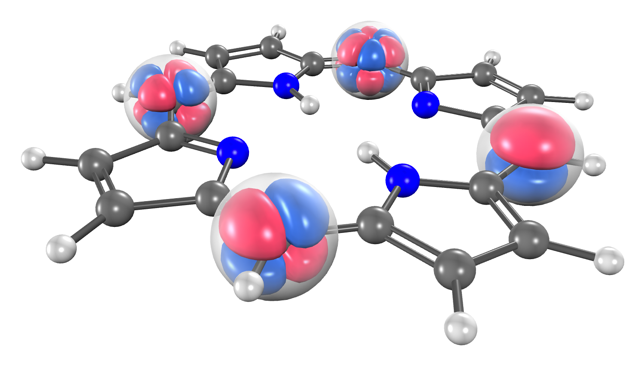
\includegraphics[width=\textwidth]{fig/SBG}
%		\end{column}
%	\end{columns}	\begin{block}{Chemist/Mulliken notation for two-electron integrals}
%		\begin{equation}
%			( \mu \nu | \lambda \sigma ) 
%			= \iint \phi_\mu^*(\alert{\br_1}) \phi_\nu(\alert{\br_1}) \frac{1}{r_{12}} \phi_\lambda^*(\blue{\br_2}) \phi_\sigma(\blue{\br_2}) d\red{\br_1} d\blue{\br_2} 
%		\end{equation}
%%		\begin{equation}
%%			( \mu \blue{\nu} \orange{||} \lambda \red{\sigma} ) = ( \mu \blue{\nu} | \lambda \red{\sigma} ) - ( \mu \red{\sigma} | \lambda \blue{\nu} )
%%		\end{equation}
%	\end{block}
%	\begin{block}{Physicist/Dirac notation for two-electron integrals}
%		\begin{equation}
%			\langle \mu \nu | \lambda \sigma \rangle 
%			= \iint \phi_\mu^*(\alert{\br_1}) \phi_\nu^*(\blue{\br_2}) \frac{1}{r_{12}} \phi_\lambda(\alert{\br_1}) \phi_\sigma(\blue{\br_2}) d\red{\br_1} d\blue{\br_2}
%		\end{equation}
%		\begin{equation}
%			\langle \mu \nu \orange{||} \blue{\lambda} \red{\sigma} \rangle =  \langle \mu \nu | \blue{\lambda} \red{\sigma} \rangle -  \langle \mu \nu |  \red{\sigma} \blue{\lambda} \rangle
%		\end{equation}
%	\end{block}
%\end{frame}


\begin{frame}{Computation of the Fock matrix and energy}
	\begin{block}{Density matrix (closed-shell system)}
		\begin{equation}
			 P_{\red{\mu \nu}} = 2 \sum_{i=1}^{N/2} C_{\red{\mu} i} C_{\red{\nu} i}^*
			\qqtext{or} 
			\boxed{\bP = 2 \bC_{\mathrm{occ}} \cdot \bC_{\mathrm{occ}}^{\dag}}
		\end{equation}
	\end{block}
	\begin{block}{Fock matrix in the AO basis (closed-shell system)}
		\begin{equation}
			F_{\red{\mu\nu}} 
			= H_{\red{\mu\nu}} 
			+ \underbrace{\sum_{\blue{\la \si}} P_{\blue{\la\si}} \rbraket{\red{\mu\nu}}{\blue{\la\si}}}_{J_{\red{\mu \nu}} = \text{ Coulomb}}
			\underbrace{ - \frac{1}{2} \sum_{\blue{\la \si}} P_{\blue{\la\si}} \rbraket{\red{\mu}\blue{\si}}{\blue{\la}\red{\nu}}}_{K_{\red{\mu \nu}} = \text{ exchange}}
		\end{equation}
	\end{block}
	\begin{block}{HF energy in the AO basis (closed-shell system)}
		\begin{equation}
			E_\text{HF} = \sum_{\red{\mu \nu}} P_{\red{\mu \nu}} H_{\red{\mu \nu}} 
			+ \frac{1}{2} \sum_{\red{\mu \nu} \blue{\la\si}} P_{\red{\mu \nu}} \qty[ \rbraket{\red{\mu \nu} }{ \blue{\lambda \sigma}} - \frac{1}{2} \rbraket{\red{\mu} \blue{\sigma} }{ \red{\lambda} \blue{\nu}} ] P_{\blue{\lambda\sigma}}
			\qqtext{or} 
			\boxed{E_\text{HF} = \frac{1}{2} \text{Tr}{\qty[\bP \cdot (\bH + \bF)]}}
		\end{equation}
	\end{block}
\end{frame}

%-----------------------------------------------------
\subsection{HF energy}
%-----------------------------------------------------
\begin{frame}{Expression of the HF energy}
	\begin{block}{Problem:}
		\violet{\textit{``Find the expression of the HF energy in terms of the one- and two-electron integrals''}}
	\end{block}
	\pause
	\begin{block}{Solution}
		\begin{equation*}
			\begin{split}
				E_\text{HF} 
				& = \sum_i^N h_{ii} + \frac{1}{2} \sum_{ij}^N (\cJ_{ij} - \cK_{ij}) 
				\\
				& = \sum_i^N  \mel{ \sum_\mu C_{\mu i} \phi_\mu }{ \hh }{  \sum_\nu C_{\nu i} \phi_\nu } 
				+ \frac{1}{2} \sum_{ij}^N \mel{ \qty(\sum_\mu C_{\mu i} \phi_\mu) \qty(\sum_\lambda C_{\lambda j} \phi_\lambda)} {} { \qty(\sum_\nu C_{\nu i} \phi_\nu) \qty(\sum_\sigma C_{\sigma j} \phi_\sigma)}
				\\
				& = \sum_{\mu \nu} P_{\mu \nu} \qty[ H_{\mu \nu} + \frac{1}{2} \sum_{\lambda \sigma} P_{\lambda \sigma} \mel{ \mu \lambda }{}{ \nu \sigma } ]
			\end{split}
		\end{equation*}
	\end{block}
\end{frame}


%-----------------------------------------------------
\subsection{SCF}
%-----------------------------------------------------
\begin{frame}{How to perform a RHF calculation in practice}
	\begin{block}{The SCF algorithm}
		\begin{enumerate}
			\item \alert{Specify molecule} $\{\bR_A\}$ and $\{Z_A\}$ and \alert{basis set} $\{\phi_\mu\}$ 
			\item Calculate integrals $S_{\mu \nu}$, $H_{\mu \nu}$ and $\braket{ \mu \nu }{ \lambda \sigma }$
			\item Diagonalize $\bS$ and compute $\bX$
			\item Choose an \alert{initial density matrix} $\bP$
			\begin{enumerate}
				\item[1.] Calculate $\bG$ and then $\bF = \bH + \bG$
				\item[2.] Compute $\bF' = \bX^\dag \cdot \bF \cdot \bX$
				\item[3.] Diagonalize $\bF'$ to obtain $\bC'$ and $\bE$
				\item[4.] Calculate $\bC= \bX \cdot  \bC'$
				\item[5.] Form a \alert{new density matrix} $\bP = 2 \bC_{\text{occ}} \cdot \bC_{\text{occ}}^\dag$
				\item[6.] \alert{Am I converged?} If not go back to 1.
			\end{enumerate}
			\item Evaluate the desired observables, including $\EHF$
		\end{enumerate}
	\end{block}
\end{frame}

\begin{frame}{Orthogonalization matrix}
	\red{We seek a matrix that orthogonalizes the AO basis, i.e., $\bX^\dag \cdot \bS \cdot  \bX = \bI$}
	\\
	\bigskip
	\begin{columns}
		\begin{column}{0.7\textwidth}
			\begin{block}{Symmetric (or L\"owdin) orthogonalization}
				\begin{equation}
					\text{$\bX =\bS^{-1/2} = \bU \cdot  \bs^{-1/2} \cdot  \bU^\dag$ is one solution.}
				\end{equation}
				\alert{Is it working?}
				\begin{equation}
					\bX^\dag \cdot \bS \cdot \bX 
					= \bS^{-1/2} \cdot \bS \cdot \bS^{-1/2} 
					= \bI \quad \green{\checkmark}
				\end{equation}
			\end{block}
			\begin{block}{Canonical orthogonalization}
				\begin{equation}
					\text{$\bX =\bU \cdot \bs^{-1/2}$ is another solution, useful when linear dependencies are present.}
				\end{equation}
					\alert{Is it working?}
				\begin{equation}
					\bX^\dag \cdot \bS \cdot  \bX 
					= \bs^{-1/2} \cdot \underbrace{\bU^{\dag} \cdot \bS \cdot \bU}_{\bs} \cdot \bs^{-1/2} 
					= \bI \quad \green{\checkmark}
				\end{equation}
			\end{block}
		\end{column}
		\begin{column}{0.3\textwidth}
			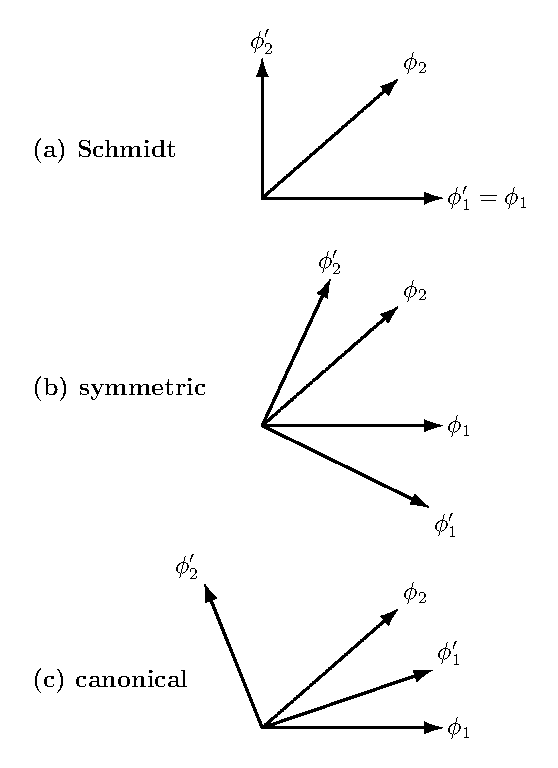
\includegraphics[width=\textwidth]{fig/ortho}
		\end{column}
	\end{columns}
\end{frame}


\begin{frame}{How to obtain a good guess for the MOs or density matrix?}
	\begin{block}{Possible initial density matrix}
		\begin{enumerate}
			\bigskip
			\item We can set \alert{$\bP = \bO$ $\Rightarrow$ $\bF = \bH$} (\alert{core guess}):\\
			$\Rightarrow$ Usually a poor guess but easy to implement
			\bigskip
			\item Use \alert{extended Huckel theory or a semi-empirical method}:\\
			$\Rightarrow$ Inexpensive, though now less common
			\bigskip
			\item Use \alert{tabulated atomic densities}:\\
			$\Rightarrow$ Superposition-of-atomic-densities (SAD) guess
			\bigskip
			\item \alert{Read the MOs of a previous calculation:}\\
			$\Rightarrow$ Very common and very useful
			\bigskip
		\end{enumerate}
	\end{block}
\end{frame}

\begin{frame}{How do I know I have converged (or not)?}
	\begin{block}{Convergence in SCF calculations}
		\begin{enumerate}
			\bigskip
			\item You can check the \alert{energy and/or the density matrix}:\\
			$\Rightarrow$ The energy/density \textbf{should not} change at convergence
			\bigskip
			\item You can check the commutator \alert{$\bF \cdot \bP \cdot \bS - \bS \cdot \bP \cdot \bF$}:\\
			$\Rightarrow$ At convergence, we have \alert{$\bF \cdot \bP \cdot \bS - \bS \cdot \bP \cdot \bF = \bO$}
			\bigskip
			\item The \alert{DIIS (direct inversion in the iterative subspace) method} is usually used to speed up convergence:\\
			$\Rightarrow$ \alert{Extrapolation of the Fock matrix} using previous iterations
			$$ \bF^{(m+1)} = \sum_{i=m-k}^{m} c_i \bF^{(i)} $$
			\bigskip
		\end{enumerate}
	\end{block}
\end{frame}

%-----------------------------------------------------
\subsection{DIIS}
%-----------------------------------------------------

\begin{frame}{SCF convergence is a nonlinear fixed-point problem}
	The SCF procedure defines an iterative map
	\begin{equation}
		\boxed{
			\bP^{(n)}
			\longrightarrow
			\bF[\bP^{(n)}]
			\longrightarrow
			\bP^{(n+1)}
		}
	\end{equation}

	At convergence,
	\begin{equation}
		\bP^{(n+1)}=\bP^{(n)}=\bP^\star
	\end{equation}

	\begin{block}{Why can the direct iteration fail?}
		\begin{itemize}
			\item The Fock matrix depends nonlinearly on the density
			\item Density updates may oscillate between different solutions
			\item The fixed-point map may be only weakly contractive---or
			      locally divergent
		\end{itemize}
	\end{block}

	\begin{alertblock}{DIIS philosophy}
		Use several previous iterations to extrapolate a Fock matrix whose
		\alert{SCF residual is as small as possible}.
	\end{alertblock}

	\vfill
	\centering
	DIIS = \alert{direct inversion in the iterative subspace}
\end{frame}

%-----------------------------------------------------

\begin{frame}{The commutator measures the SCF error}
	The Roothaan--Hall equations are
	\begin{equation}
		\bF \cdot \bC = \bS \cdot \bC \cdot \bE
	\end{equation}

	At self-consistency, the density and Fock matrices commute in the
	AO metric:
	\begin{equation}
		\boxed{
			\be^{(n)}
			=
			\bF^{(n)} \cdot \bP^{(n)} \cdot \bS
			-
			\bS \cdot \bP^{(n)} \cdot \bF^{(n)}
		}
	\end{equation}

	\begin{equation}
		\bP^{(n)}=\bP^\star
		\qquad\Longrightarrow\qquad
		\be^{(n)}=\bO.
	\end{equation}

	\begin{block}{In an orthonormal basis}
		If $\bX^\dagger \cdot \bS \cdot \bX = \bI$, the transformed residual is
		\begin{equation}
			\widetilde{\be}^{(n)}
			=
			\bX^\dagger \cdot \be^{(n)} \cdot \bX
			=
			\comm{
				\widetilde{\bF}^{(n)}
			}{
				\widetilde{\bP}^{(n)}
			}
		\end{equation}
	\end{block}

	\centering
	\alert{The residual vanishes when the occupied space is invariant under
	the Fock operator}
\end{frame}

%-----------------------------------------------------

\begin{frame}{DIIS stores Fock matrices and their residuals}
	Let $m$ be the maximum size of the DIIS subspace.

	\medskip
	\centering
	\small
	\renewcommand{\arraystretch}{1.35}
	\begin{tabularx}{0.95\textwidth}{
		>{\bfseries}l
		>{\centering\arraybackslash}m{0.22\textwidth}
		X
	}
		\toprule
		Stored quantity & Size & Purpose \\
		\midrule
		$\bF^{(i)}$
		& $\mathcal{O}(K^2)$
		& Used to construct the extrapolated Fock matrix
		\\

		$\be^{(i)}$
		& $\mathcal{O}(K^2)$
		& Measures the lack of self-consistency at iteration $i$
		\\

		$B_{ij}$
		& $\mathcal{O}(m^2)$
		& Contains the scalar products between error vectors
		\\

		$c_i$
		& $\mathcal{O}(m)$
		& DIIS extrapolation coefficients
		\\
		\bottomrule
	\end{tabularx}

	\begin{equation}
		\boxed{
			\text{storage}
			\sim
			2mK^2
			\text{ floating-point numbers}
		}
	\end{equation}

	\begin{itemize}
		\item A small rolling subspace is normally sufficient:
		      commonly $m\approx6$--$10$
		\item When the subspace is full, an old or redundant pair
		      $\{\bF^{(i)},\be^{(i)}\}$ is removed
	\end{itemize}

	\begin{block}{UHF calculations}
		The alpha and beta residuals may be concatenated,
		\[
			\be^{(i)}
			=
			\left(
				\be_\alpha^{(i)},
				\be_\beta^{(i)}
			\right),
		\]
		and the same coefficients are applied to both Fock matrices.
	\end{block}
\end{frame}

%-----------------------------------------------------

\begin{frame}{DIIS searches for the smallest residual in the subspace}
	Using the $m$ stored iterations, DIIS constructs
	\begin{align}
		\bF^\text{DIIS}
		&=
		\sum_{i=1}^{m}c_i\bF^{(i)},
		\\
		\be^\text{DIIS}
		&\approx
		\sum_{i=1}^{m}c_i\be^{(i)}.
	\end{align}

	The coefficients minimize the residual norm:
	\begin{equation}
		\boxed{
			\min_{\bc}
			\norm{
				\sum_{i=1}^{m}c_i\be^{(i)}
			}_F^2
			\qquad
			\text{subject to}
			\qquad
			\sum_{i=1}^{m}c_i=1
		}
	\end{equation}

	Define the DIIS overlap matrix
	\begin{equation}
		B_{ij}
		=
		\braket{\be^{(i)}}{\be^{(j)}}
		=
		\Tr[
			\be^{(i)\dagger}\be^{(j)}
		].
	\end{equation}

	Then
	\begin{equation}
		\norm{\be^\text{DIIS}}_F^2
		=
		\sum_{ij}c_iB_{ij}c_j
		=
		\bc^\mathsf{T}\bB\bc.
	\end{equation}

	\begin{alertblock}{Important}
		The constraint $\sum_i c_i=1$ defines an
		\alert{affine extrapolation}. The coefficients need not be positive.
	\end{alertblock}
\end{frame}

%-----------------------------------------------------

\begin{frame}{The DIIS weights come from a small augmented system}
	Introduce a Lagrange multiplier $\lambda$:
	\begin{equation}
		\mathcal{L}(\bc,\lambda)
		=
		\bc^\mathsf{T}\bB\bc
		-
		2\lambda
		\left(
			\boldsymbol{1}^\mathsf{T}\bc-1
		\right).
	\end{equation}

	Stationarity gives
	\begin{equation}
		\bB\bc-\lambda\boldsymbol{1}=\bO,
		\qquad
		\boldsymbol{1}^\mathsf{T}\bc=1.
	\end{equation}

	Therefore, the weights are obtained from
	\begin{equation}
		\boxed{
		\begin{pmatrix}
			B_{11} & \cdots & B_{1m} & -1 \\
			\vdots & \ddots & \vdots & \vdots \\
			B_{m1} & \cdots & B_{mm} & -1 \\
			-1     & \cdots & -1     & 0
		\end{pmatrix}
		\begin{pmatrix}
			c_1 \\ \vdots \\ c_m \\ \lambda
		\end{pmatrix}
		=
		\begin{pmatrix}
			0 \\ \vdots \\ 0 \\ -1
		\end{pmatrix}
		}
	\end{equation}

	Once the $c_i$ are known,
	\begin{equation}
		\boxed{
			\bF^\text{DIIS}
			=
			\sum_{i=1}^{m}c_i\bF^{(i)}
		}
	\end{equation}

	\centering
	The linear system has dimension only $(m+1)\times(m+1)$.
\end{frame}

%-----------------------------------------------------

\begin{frame}{One DIIS cycle uses the complete iteration history}
	\small
	\begin{enumerate}
		\item Start from the current density $\bP^{(n)}$

		\item Build the corresponding Fock matrix
		      \[
			      \bF^{(n)}=\bF[\bP^{(n)}]
		      \]

		\item Evaluate the commutator residual
		      \[
			      \be^{(n)}
			      =
			      \bF^{(n)}\bP^{(n)}\bS
			      -
			      \bS\bP^{(n)}\bF^{(n)}
		      \]

		\item Store the pair
		      $\{\bF^{(n)},\be^{(n)}\}$ and update the DIIS subspace

		\item Construct $\bB$, solve the augmented linear system, and obtain
		      the coefficients $\{c_i\}$

		\item Extrapolate the Fock matrix
		      \[
			      \bF^\text{DIIS}
			      =
			      \sum_i c_i\bF^{(i)}
		      \]

		\item Solve
		      \[
			      \bF^\text{DIIS}\bC
			      =
			      \bS\bC\bepsilon
		      \]
		      and form the next density $\bP^{(n+1)}$
	\end{enumerate}

	\begin{alertblock}{Convergence tests}
		Check the energy change, density change, and residual norm;
		do not rely on only one of them.
	\end{alertblock}
\end{frame}

%-----------------------------------------------------

\begin{frame}{DIIS is powerful, but the subspace can become unstable}
	\small
	\centering
	\renewcommand{\arraystretch}{1.35}
	\begin{tabularx}{0.97\textwidth}{
		>{\bfseries}m{0.21\textwidth}
		m{0.31\textwidth}
		X
	}
		\toprule
		Symptom & Likely cause & Possible response \\
		\midrule
		Early oscillations
		& Iterates are outside the local convergence region
		& Delay DIIS; use damping or level shifting
		\\

		Nearly singular $\bB$
		& Stored residuals are nearly linearly dependent
		& Remove a redundant vector, restart, or use an SVD cutoff
		\\

		Very large $c_i$
		& Unstable extrapolation outside the sampled region
		& Reset or reduce the DIIS subspace
		\\

		Convergence to the wrong state
		& Orbital occupations or roots change during the iteration
		& Use state tracking or the maximum-overlap method
		\\
		\bottomrule
	\end{tabularx}

	\begin{block}{A robust practical strategy}
		\begin{itemize}
			\item Begin with damping, level shifting, EDIIS, or ADIIS
			\item Switch to commutator DIIS near the solution
			\item Keep only a small, well-conditioned history
		\end{itemize}
	\end{block}

	\begin{alertblock}{DIIS minimizes a residual---not the energy}
		The extrapolated energy is not guaranteed to decrease monotonically.
	\end{alertblock}
\end{frame}

%-----------------------------------------------------

\begin{frame}{DIIS variants target different convergence regimes}
	\begin{columns}[T,onlytextwidth]
		\begin{column}{0.48\textwidth}
			\begin{block}{CDIIS}
				\begin{itemize}
					\item Uses the commutator residual
					\item Very efficient close to self-consistency
					\item May be unstable far from the solution
				\end{itemize}
			\end{block}

			\begin{block}{EDIIS}
				\begin{itemize}
					\item Uses energy-based convex mixing
					\item More robust in the early SCF iterations
					\item Usually slower near convergence
				\end{itemize}
			\end{block}
		\end{column}

		\begin{column}{0.48\textwidth}
			\begin{block}{ADIIS}
				\begin{itemize}
					\item Uses an approximate SCF energy model
					\item Designed for the difficult initial regime
					\item Often combined with CDIIS
				\end{itemize}
			\end{block}

			\begin{block}{Hybrid strategy}
				\[
					\text{EDIIS/ADIIS}
					\quad\longrightarrow\quad
					\text{CDIIS}
				\]
				\centering
				Robust far away; fast close to the solution.
			\end{block}
		\end{column}
	\end{columns}

	\begin{alertblock}{Take-home message}
		DIIS accelerates SCF convergence by finding an affine combination
		of previous Fock matrices whose extrapolated residual is minimal.
	\end{alertblock}

	\vfill
	\centering
	\pub{
		P.~Pulay, Chem.\ Phys.\ Lett.\ \textbf{73}, 393 (1980);
		J.\ Comput.\ Chem.\ \textbf{3}, 556 (1982).
	}
\end{frame}

%-----------------------------------------------------
\subsection{Properties}
%-----------------------------------------------------
\begin{frame}{Dipole moments}
	\begin{block}{Classical vs Quantum}
		\begin{equation}
			\boldsymbol{\mu} = (\mu_x,\mu_y,\mu_z)
			= \underbrace{\green{\sum_i q_i \br_i}}_{\text{\green{classical definition}}}
		\end{equation}
		\begin{equation}
			\boldsymbol{\mu} = (\mu_x,\mu_y,\mu_z)
			= \underbrace{\red{\mel{\Psi_0}{- \sum_i^N \br_i}{\Psi_0}}}_{\text{\red{electrons}}} + \underbrace{\blue{\sum_A^M Z_A \bR_A}}_{\text{\blue{nuclei}}}
			=  \red{- \sum_{\mu \nu} P_{\mu\nu} \rmel{\nu}{\br}{\mu}} + \blue{\sum_A^M Z_A \bR_A}
		\end{equation}
	\end{block}
	\begin{block}{Vector components}
		\begin{equation}
			\mu_x = \red{- \sum_{\mu \nu} P_{\mu\nu} \rmel{\nu}{x}{\mu}} + \blue{\sum_A^M Z_A X_A}
			\qq{with}
			\underbrace{\rbraket{\nu}{x}{\mu}}_{\text{one-electron integrals}} = \int \phi_\nu^*(\br) \,x\, \phi_\mu(\br) \dd{\br}  
		\end{equation}
	\end{block}
\end{frame}

\begin{frame}{Charge analysis}
	\begin{block}{Electron density}
		\begin{equation}
			\rho(\br) = \sum_{\mu\nu} \phi_\mu(\br) P_{\mu\nu} \phi_\nu(\br) 
			\qq{with}
			\int \rho(\br) d\br = N
			\qq{$\Rightarrow$}
			N = \sum_{\mu\nu} P_{\mu\nu} S_{\nu\mu} = \sum_\mu (\bP \cdot \bS)_{\mu\mu} = \Tr(\bP \cdot \bS)
		\end{equation}
	\end{block}
	\begin{block}{Mulliken population analysis}
		Assuming that the basis functions are atom-centered
		\begin{equation}
			\underbrace{\blue{q_A^\text{Mulliken}}}_{\text{net charge on $A$}} = Z_A - \sum_{\mu \in A} (\bP \cdot \bS)_{\mu\mu}
		\end{equation}
	\end{block}
	\begin{block}{L{\"o}wdin population analysis}
		Because $\Tr(\bA \cdot \bB) = \Tr(\bB \cdot \bA)$, we have, for any $\alpha$, 
		$N = \sum_{\mu} (\bS^{\alpha} \cdot \bP \cdot \bS^{1-\alpha})_{\mu\mu}$
		\begin{equation}
			\qq*{For \red{$\alpha = 1/2$}, we get:}
			N = \sum_{\mu} (\bS^{1/2} \cdot \bP \cdot \bS^{1/2})_{\mu\mu}
			\qq{$\Rightarrow$}
			\red{q_A^\text{L{\"o}wdin}} = Z_A - \sum_{\mu \in A} (\bS^{1/2} \cdot \bP \cdot \bS^{1/2})_{\mu\mu}
		\end{equation}
	\end{block}
\end{frame}

%-----------------------------------------------------
\section{Unrestricted HF}
%-----------------------------------------------------
%-----------------------------------------------------
\subsection{UHF}
%-----------------------------------------------------
\begin{frame}{Unrestricted HF (UHF)}
	\begin{block}{How to model open-shell systems?}
		\begin{itemize}
			\item For open-shell systems one uses \alert{unrestricted spin orbitals}
			\begin{equation}
				\chi_p^\text{UHF}(\bx) = 
				\begin{cases}
					\alpha(\omega) \blue{\psi_p^\alpha(\br)}
					\\
					\beta(\omega) \red{\psi_p^\beta(\br)}
				\end{cases}
			\end{equation}		
			\item UHF may break spin symmetry: the determinant need not be an eigenfunction of $\chS^2$
			\item The HF wave function is no longer a pure spin function
			\item Singlets are contaminated by triplets, quintets, etc
			\item Doublets are contaminated by quartets, sextuplets, etc
			\item Generalized HF also allows spin mixing and need not preserve $\chS_z$
			\begin{equation}
				\chi_p^\text{GHF}(\bx) = \alpha(\omega) \blue{\psi_p^\alpha(\br)} + \beta(\omega) \red{\psi_p^\beta(\br)}
				\qq{$\Rightarrow$ \alert{two-component spinor}}
			\end{equation}
		\end{itemize}
	\end{block}
\end{frame}

%\begin{frame}{RHF, ROHF and UHF}
%	\center
%	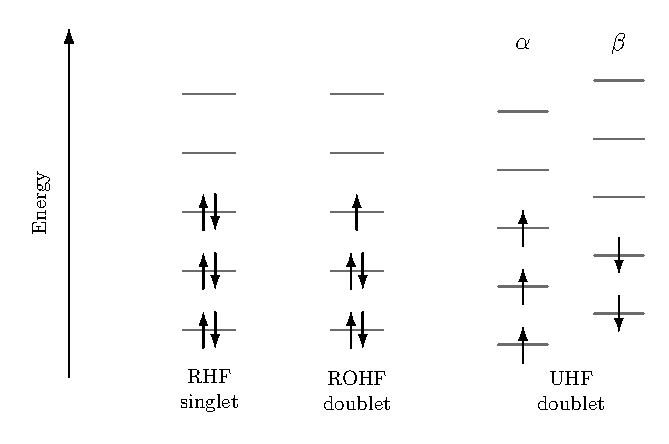
\includegraphics[width=0.4\textwidth]{fig/RHF_UHF}
%	\begin{itemize}
%		\item RHF = \orange{Restricted} Hartree-Fock
%		\item UHF = \red{Unrestricted} Hartree-Fock
%		\item ROHF = \blue{Restricted Open-shell} Hartree-Fock
%	\end{itemize}
%\end{frame}

%-----------------------------------------------------
%\subsection{UHF wave function}
%-----------------------------------------------------
%\begin{frame}{The UHF wave function}
%	\begin{block}{Slater determinants for UHF}
%		\small
%		\begin{equation*}
%			\Psi_\text{UHF}%(\br_1,\ldots,\br_N) 
%			= 
%			\underbrace{
%			\frac{1}{\sqrt{N^\alpha!}}
%			\begin{vmatrix}
%			\psi_1^\alpha(\br_1)	&	\cdots	&	\psi_{N^\alpha}^\alpha(\br_1)	\\
%			\vdots				&	\ddots	&	\vdots			\\
%			\psi_1^\alpha(\br_{N^\alpha})	&	\cdots	&	\psi_{N^\alpha}^\alpha(\br_{N^\alpha})	\\
%			\end{vmatrix}
%			}_{\orange{\Psi^\alpha(\br_1,\ldots,\br_{N^\alpha}) }}
%			\underbrace{
%			\frac{1}{\sqrt{N^\beta!}}
%			\begin{vmatrix}
%			\psi_1^\beta(\br_{N^\alpha+1})	&	\cdots	&	\psi_{N^\beta}^\beta(\br_{N^\alpha+1})	\\
%			\vdots				&	\ddots	&	\vdots			\\
%			\psi_1^\beta(\br_{N})	&	\cdots	&	\psi_{N^\beta}^\beta(\br_{N})	\\
%			\end{vmatrix}
%			}_{\alert{\Psi^\beta(\br_{N^\alpha+1},\ldots,\br_{N}) }}
%		\end{equation*}
%		\normalsize
%		\begin{itemize}
%			\item The UHF wave function is \violet{a product of two determinants}
%			\begin{itemize}
%				\item One for the \orange{spin-up electrons} $\orange{\Psi^\alpha(\br_1,\ldots,\br_{N^\alpha}) }$
%				\item One for the \alert{spin-down electrons} $\alert{\Psi^\beta(\br_{N^\alpha+1},\ldots,\br_{N}) }$
%			\end{itemize}
%			\item The \alert{Pauli exclusion principle} only requires the \blue{wave function to be antisymmetric wrt the exchange of two same-spin electrons}
%		\end{itemize}
%	\end{block}
%\end{frame}

%-----------------------------------------------------
\subsection{UHF equations}
%-----------------------------------------------------
\begin{frame}{Unrestricted Hartree--Fock equations}
	\small
	\begin{block}{UHF equations for unrestricted spin orbitals}
		\bigskip
		\alert{To minimize the UHF energy}, the unrestricted spatial orbitals must be eigenfunctions of the \alert{$\alpha$ and $\beta$ Fock operators}:
		\begin{align}
			& \boxed{
			\orange{f^\alpha(\br_1) \psi_i^\alpha(\br_1) = \epsilon_i^\alpha \psi_i^\alpha(\br_1)}
			}
			& 
			& \boxed{
			\alert{f^\beta(\br_1) \psi_i^\beta(\br_1) = \epsilon_i^\beta \psi_i^\beta(\br_1)}
			}
		\end{align}
		where
		\begin{align}
			\orange{f^\alpha(\br_1)} & = h(\br_1) + \sum_{i}^{N^\alpha} [ \orange{J_i^\alpha(\br_1) - K_i^\alpha(\br_1)} ]  + \sum_{i}^{N^\beta} \alert{J_i^\beta(\br_1)}
			\\
			\alert{f^\beta(\br_1)} & = h(\br_1) + \sum_{i}^{N^\beta} [ \alert{J_i^\beta(\br_1) - K_i^\beta(\br_1)} ]  + \sum_{i}^{N^\alpha} \orange{J_i^\alpha(\br_1)}
		\end{align}	
		The \blue{Coulomb} and \violet{Exchange} operators are
		\begin{align}
			\blue{J_i^\sigma(\br_1)} & = \int \psi_i^{\sigma *}(\br_2) r_{12}^{-1} \psi_i^\sigma(\br_2) \dd{\br_2} 
			& 
			\violet{K_i^\sigma(\br_1)} \psi_j^\sigma(\br_1) & =  \qty[ \int \psi_i^{\sigma *}(\br_2) r_{12}^{-1} \psi_j^\sigma(\br_2) \dd{\br_2} ] \psi_i^\sigma(\br_1)
		\end{align}		
	\end{block}
\end{frame}

\begin{frame}{The UHF energy}
	\begin{block}{UHF energy}
		\bigskip
		The UHF energy comprises three contributions:	
		\begin{equation}
			E_\text{UHF} = \orange{E_\text{UHF}^{\alpha\alpha}} + \red{E_\text{UHF}^{\beta\beta}} + \violet{E_\text{UHF}^{\alpha\beta}}	
		\end{equation}		
		which yields
		{\small
		\begin{equation}
			\boxed{
			E_\text{UHF} = 
			\orange{\sum_{i}^{N^\alpha} h_{ii}^\alpha 
			+ \frac{1}{2} \sum_{ij}^{N^\alpha} (J_{ij}^{\alpha\alpha} - K_{ij}^{\alpha\alpha})}
			+ \red{\sum_{i}^{N^\beta} h_{ii}^\beta 
			+ \frac{1}{2} \sum_{ij}^{N^\beta} (J_{ij}^{\beta\beta} - K_{ij}^{\beta\beta})}
			+ \violet{\sum_{i}^{N^\alpha} \sum_{j}^{N^\beta} J_{ij}^{\alpha\beta}} 
			}
		\end{equation}}	
		The matrix elements are given by			
		\begin{align}
			h_{ii}^\sigma & = \mel{ \psi_i^\sigma }{ h }{ \psi_i^\sigma } 
			& 
			J_{ij}^{\sigma\sigma'} & = \braket*{ \psi_i^\sigma \psi_j^{\sigma'} }{  \psi_i^\sigma \psi_j^{\sigma'} } 
			&
			K_{ij}^{\sigma\sigma} & = \braket*{ \psi_i^\sigma \psi_j^\sigma }{  \psi_j^\sigma \psi_i^\sigma } 
		\end{align}	
		Note that \blue{$K_{ij}^{\alpha\beta} = 0$} $\Leftrightarrow$ \alert{there is no exchange between opposite-spin electrons}
	\end{block}
\end{frame}

\begin{frame}{UHF energy of the \ce{Li} atom}
	\begin{block}{Problem}
	\violet{\textit{``Write down the UHF energy of the doublet state of the lithium atom''}}
	\end{block}
	\pause
	\begin{block}{Solution}
%		The UHF wave function for the doublet state of \ce{Li} is
%		\begin{equation*}
%			\Psi_\text{UHF}(\br_1,\br_2,\br_3) 
%			= \frac{1}{\sqrt{2}}
%			\begin{vmatrix}
%				\psi_1^\alpha(\br_1)	&	\psi_2^\alpha(\br_1)	\\
%				\psi_1^\alpha(\br_2)	&	\psi_2^\alpha(\br_2)	\\
%			\end{vmatrix}
%			\psi_1^\beta(\br_3)
%		\end{equation*}
%		while the corresponding energy is
		\begin{equation*}
			E_\text{UHF} = h_1^\alpha + h_1^\beta + h_2^\alpha + J_{12}^{\alpha\alpha} - K_{12}^{\alpha\alpha} + J_{11}^{\alpha\beta} + J_{21}^{\alpha\beta}
		\end{equation*}
	\end{block}
\end{frame}

%-----------------------------------------------------
\subsection{Pople-Nesbet}
%-----------------------------------------------------
\begin{frame}{The Pople-Nesbet Equations}
	\small
	\begin{block}{Expansion of the unrestricted spin orbitals in a basis}
		\begin{align}
			\psi_i^\alpha (\br) & = \sum_{\mu=1}^K \blue{C_{\mu i}^\alpha} \phi_{\mu} (\br)
			& 
			\psi_i^\beta (\br) & = \sum_{\mu=1}^K \violet{C_{\mu i}^\beta} \phi_{\mu} (\br)
		\end{align}
	\end{block}
	\begin{block}{The Pople-Nesbet equations}
		\begin{align}
			\orange{\bF^\alpha} \cdot \blue{\bC^\alpha} & = \bS \cdot  \blue{\bC^\alpha} \cdot  \bE^\alpha
			& 
			\red{\bF^\beta} \cdot \violet{\bC^\beta} & = \bS \cdot  \violet{\bC^\beta} \cdot  \bE^\beta
		\end{align}
		\begin{gather}
			\orange{F_{\mu \nu}^\alpha} 
			= H_{\mu \nu} 
			+ \sum_{\lambda \sigma} \blue{P_{\lambda \sigma}^\alpha} [ \rbraket{\mu \nu }{ \sigma \lambda} - \rbraket{\mu \lambda }{ \sigma \nu} ] 
			+ \sum_{\lambda \sigma} \violet{P_{\lambda \sigma}^\beta} \rbraket{\mu \nu }{ \sigma \lambda} 
			\\
			\red{F_{\mu \nu}^\beta}
			= H_{\mu \nu} 
			+ \sum_{\lambda \sigma} \violet{P_{\lambda \sigma}^\beta} [ \rbraket{\mu \nu }{ \sigma \lambda} - \rbraket{\mu \lambda }{ \sigma \nu} ] 
			+ \sum_{\lambda \sigma} \blue{P_{\lambda \sigma}^\alpha} \rbraket{\mu \nu }{ \sigma \lambda} 		
		\end{gather}
		$\orange{\bF^\alpha}$ and $\red{\bF^\beta}$ are both functions of $\blue{\bC^\alpha}$ and $\violet{\bC^\beta}$
		$\Rightarrow$ \alert{There's a coupling between $\alpha$ and $\beta$ orbitals!}
	\end{block}
\end{frame}

\begin{frame}{Unrestricted Density Matrices}
	\begin{block}{Spin-up and spin-down density matrices}
		\begin{align}
			&\boxed{
				\orange{P_{\mu \nu}^\alpha} = \sum_{i=1}^{N^\alpha} C_{\mu i}^\alpha C_{\nu i}^{\alpha *}
				\quad \Leftrightarrow \quad \orange{\bP^\alpha}
			}
			&
			&\boxed{
				\alert{P_{\mu \nu}^\beta} = \sum_{i=1}^{N^\beta} C_{\mu i}^\beta C_{\nu i}^{\beta *}
				\quad \Leftrightarrow \quad \alert{\bP^\beta}
			}
		\end{align}
	\end{block}
	\begin{block}{Properties of the density $(\sigma = \alpha \text{ or } \beta)$}
		\begin{align}
			\rho^\sigma(\br) & = \sum_{\mu \nu} \phi_{\mu}(\br) P_{\mu \nu}^\sigma \phi_{\nu}(\br)
			&
			\int \rho^\sigma(\br) d\br & = N^\sigma
		\end{align}
	\end{block}
	\begin{block}{Total and Spin density matrices}
		\begin{align}
			\underbrace{\blue{\bP^\text{T}}}_{\blue{\text{Charge density}}} & = \orange{\bP^\alpha} + \alert{\bP^\beta}
			&
			\underbrace{\violet{\bP^\text{S}}}_{\violet{\text{Spin density}}} & = \orange{\bP^\alpha} - \alert{\bP^\beta}
		\end{align}
	\end{block}
\end{frame}

%-----------------------------------------------------
\subsection{SCF for UHF}
%-----------------------------------------------------
\begin{frame}{How to perform a UHF calculation in practice}
	\begin{block}{The SCF algorithm}
		\begin{enumerate}
			\item \alert{Specify molecule} $\{\bR_A\}$ and $\{Z_A\}$ and \alert{basis set} $\{\phi_\mu\}$ \alert{(same as RHF)}
			\item Calculate integrals $S_{\mu \nu}$, $H_{\mu \nu}$ and $\braket{ \mu \nu }{ \lambda \sigma }$ \alert{(same as RHF)}
			\item Diagonalize $\bS$ and compute $\bX$ \alert{(same as RHF)}
			\item Choose \alert{initial density matrices} $\bP^\alpha$ and $\bP^\beta$
			\begin{enumerate}
				\item[1a.] Calculate $\bG^\alpha$ and then $\bF^\alpha = \bH + \bG^\alpha$
				\item[1b.] Calculate $\bG^\beta$ and then $\bF^\beta = \bH + \bG^\beta$
				\item[2.] Compute $(\bF^\alpha)' = \bX^\dag \cdot  \bF^\alpha \cdot \bX$ and $(\bF^\beta)' = \bX^\dag \cdot  \bF^\beta \cdot \bX$
				\item[3a.] Diagonalize $(\bF^\alpha)'$ to obtain $(\bC^\alpha)'$ and $\bE^\alpha$
				\item[3b.] Diagonalize $(\bF^\beta)'$ to obtain $(\bC^\beta)'$ and $\bE^\beta$
				\item[4.] Calculate $\bC^\alpha= \bX \cdot (\bC^\alpha)'$ and  $\bC^\beta= \bX \cdot (\bC^\beta)'$
				\item[5.] Form the \alert{new density matrices} $\bP^\alpha$ and $\bP^\beta$, and compute $\bP^\text{T} = \bP^\alpha + \bP^\beta$
				\item[6.] \alert{Am I converged?} If not go back to 1.
			\end{enumerate}
			\item Evaluate the desired observables, including $E_\text{UHF}$
		\end{enumerate}
	\end{block}
\end{frame}

%-----------------------------------------------------
\subsection{Dissociation of \ce{H2}}
%-----------------------------------------------------

\newcommand{\HtwoOrbitalPlot}[1]{%
	\begin{tikzpicture}
		\begin{axis}[
			width=\linewidth,
			height=0.48\textheight,
			xmin=-3,xmax=3,
			ymin=-0.05,ymax=1.48,
			axis x line=middle,
			axis y line=none,
			xtick=\empty,
			ytick=\empty,
			clip=false,
			samples=120,
			domain=-3:3,
		]
			\addplot[hfBlue,very thick]
				{cos(#1)*(exp(-1.7*(x+1.15)^2)+exp(-1.7*(x-1.15)^2))/sqrt(2)
				+sin(#1)*(exp(-1.7*(x+1.15)^2)-exp(-1.7*(x-1.15)^2))/sqrt(2)};
			\addplot[hfRed,very thick,dashed]
				{cos(#1)*(exp(-1.7*(x+1.15)^2)+exp(-1.7*(x-1.15)^2))/sqrt(2)
				-sin(#1)*(exp(-1.7*(x+1.15)^2)-exp(-1.7*(x-1.15)^2))/sqrt(2)};
			\addplot[only marks,mark=*,mark size=1.7pt,hfInk]
				coordinates {(-1.15,0) (1.15,0)};
			\node[below,font=\scriptsize] at (axis cs:-1.15,0) {$A$};
			\node[below,font=\scriptsize] at (axis cs: 1.15,0) {$B$};
		\end{axis}
	\end{tikzpicture}%
}

%-----------------------------------------------------
\begin{frame}{Minimal-basis \ce{H2} is a complete Hartree--Fock laboratory}
	Start from one normalized $1s$ function on each atom,
	$\phi_A$ and $\phi_B$, with $S=\braket{\phi_A}{\phi_B}$.

	\begin{equation}
		\boxed{
			\psi_g
			=
			\frac{\phi_A+\phi_B}{\sqrt{2(1+S)}},
			\qquad
			\psi_u
			=
			\frac{\phi_A-\phi_B}{\sqrt{2(1-S)}}
		}
	\end{equation}

	\begin{columns}[T,onlytextwidth]
		\begin{column}{0.48\textwidth}
			\begin{block}{What the model retains}
				\begin{itemize}
					\item Bond formation through $g/u$ mixing
					\item Static correlation upon dissociation
					\item Restricted and symmetry-broken HF solutions
				\end{itemize}
			\end{block}
		\end{column}
		\begin{column}{0.48\textwidth}
			\begin{block}{Why it is special}
				For two electrons in two spatial orbitals, the UHF problem reduces to
				\alert{one orbital-rotation angle}.
			\end{block}
		\end{column}
	\end{columns}

	\centering
	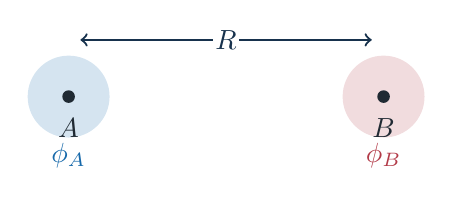
\begin{tikzpicture}[x=1cm,y=1cm]
		\fill[hfBlue!18] (-2.0,0) circle (0.52);
		\fill[hfRed!18]  ( 2.0,0) circle (0.52);
		\fill[hfInk] (-2.0,0) circle (0.08) node[below=0.15cm] {$A$};
		\fill[hfInk] ( 2.0,0) circle (0.08) node[below=0.15cm] {$B$};
		\draw[hfNavy,thick,<->] (-1.85,0.72)--(1.85,0.72)
			node[midway,fill=white,inner sep=1pt] {$R$};
		\node[hfBlue] at (-2.0,-0.75) {$\phi_A$};
		\node[hfRed]  at ( 2.0,-0.75) {$\phi_B$};
	\end{tikzpicture}
\end{frame}

%-----------------------------------------------------
\begin{frame}{RHF is qualitatively correct near equilibrium---but not at dissociation}
	The closed-shell RHF wave function doubly occupies the bonding orbital:
	\begin{equation}
		\ket{\Psi_\text{RHF}}
		=
		\ket{\psi_g\Bar{\psi}_g},
		\qquad
		E_\text{RHF}
		=
		2h_{gg}+J_{gg}+\frac{1}{R}.
	\end{equation}

	At large $R$, where $S\rightarrow0$,
	\begin{equation}
		\psi_g(1)\psi_g(2)
		\longrightarrow
		\frac{1}{2}
		\left[
			\underbrace{
				\phi_A(1)\phi_B(2)+\phi_B(1)\phi_A(2)
			}_{\text{covalent}}
			+
			\underbrace{
				\phi_A(1)\phi_A(2)+\phi_B(1)\phi_B(2)
			}_{\text{ionic}}
		\right].
	\end{equation}

	\begin{block}{The restricted dissociation error}
		RHF retains \alert{50\% ionic character} at $R\rightarrow\infty$.
		Both electrons are forced to share the same spatial orbital, so the RHF
		energy lies above the energy of two separated H atoms.
	\end{block}

	\centering
	$\Rightarrow$ \alert{The missing ingredient is left--right correlation}
\end{frame}

%-----------------------------------------------------
\begin{frame}{UHF introduces a single spin-polarization angle}
	Preserve $M_S=0$, but allow the $\alpha$ and $\beta$ electrons to occupy
	different spatial orbitals:
	\begin{equation}
		\boxed{
		\begin{aligned}
			\psi^\alpha(\theta)
				&=\cos\theta\,\psi_g+\sin\theta\,\psi_u,\\
			\psi^\beta(\theta)
				&=\cos\theta\,\psi_g-\sin\theta\,\psi_u.
		\end{aligned}}
	\end{equation}

	\begin{columns}[T,onlytextwidth]
		\begin{column}{0.48\textwidth}
			\begin{block}{$\theta=0$: restricted solution}
				\begin{equation}
					\psi^\alpha=\psi^\beta=\psi_g.
				\end{equation}
				The UHF determinant collapses to RHF.
			\end{block}
		\end{column}
		\begin{column}{0.48\textwidth}
			\begin{block}{$\theta\rightarrow\pi/4$: localized solution}
				At dissociation,
				\begin{equation}
					\psi^\alpha\rightarrow\phi_A,
					\qquad
					\psi^\beta\rightarrow\phi_B.
				\end{equation}
				Opposite spins occupy opposite atoms.
			\end{block}
		\end{column}
	\end{columns}

	\begin{equation}
		\braket{\psi^\alpha}{\psi^\beta}=\cos(2\theta).
	\end{equation}

	\centering
	The two choices $\pm\theta$ are degenerate and exchange the spin localization.
\end{frame}

%-----------------------------------------------------
\begin{frame}{Stretching the bond continuously localizes the UHF orbitals}
	\small
	The mixing angle transfers opposite-spin density toward opposite nuclei.

	\begin{columns}[T,onlytextwidth]
		\begin{column}{0.32\textwidth}
			\centering
			\textbf{$\theta=0^\circ$: RHF limit}

			\HtwoOrbitalPlot{0}

			$\psi^\alpha=\psi^\beta=\psi_g$
		\end{column}
		\begin{column}{0.32\textwidth}
			\centering
			\textbf{$0<\theta<45^\circ$: polarization}

			\HtwoOrbitalPlot{22.5}

			$\alpha$ shifts to $A$; $\beta$ shifts to $B$
		\end{column}
		\begin{column}{0.32\textwidth}
			\centering
			\textbf{$\theta=45^\circ$: dissociation}

			\HtwoOrbitalPlot{45}

			$\psi^\alpha\to\phi_A$; $\psi^\beta\to\phi_B$
		\end{column}
	\end{columns}

	\vspace{0.5em}
	\centering
	\tikz[baseline=-0.5ex]{
		\draw[hfBlue,very thick] (0,0)--(0.7,0);
		\node[right,hfInk,font=\scriptsize] at (0.72,0) {$\psi^\alpha$};
		\draw[hfRed,very thick,dashed] (2.0,0)--(2.7,0);
		\node[right,hfInk,font=\scriptsize] at (2.72,0) {$\psi^\beta$};
	}

	\vspace{0.5em}
	\alert{Orbital localization is continuous; the onset of the nonzero angle is the bifurcation.}
\end{frame}

%-----------------------------------------------------
\begin{frame}{The UHF energy is an analytic function of the mixing angle}
	\small
	With $J_{pq}=(pp|qq)$ and $K_{pq}=(pq|pq)$,
	\begin{align}
		E_\text{UHF}(\theta)-\frac{1}{R}
		={}&
		2\cos^2\theta\,h_{gg}
		+2\sin^2\theta\,h_{uu}
		+\cos^4\theta\,J_{gg}
		+\sin^4\theta\,J_{uu}
		\notag\\
		&+2\sin^2\theta\cos^2\theta
		\left(J_{gu}-2K_{gu}\right).
	\end{align}

	Besides the restricted stationary point $\theta=0$, a broken-symmetry
	stationary solution satisfies
	\begin{equation}
		\boxed{
			\cos(2\theta)
			=
			\frac{
				h_{uu}-h_{gg}+J_{uu}-J_{gu}+2K_{gu}
			}{
				J_{gg}+J_{uu}-2J_{gu}+4K_{gu}
			}
		}.
	\end{equation}

	\begin{columns}[T,onlytextwidth]
		\begin{column}{0.48\textwidth}
			\begin{block}{Short bond}
				Only the minimum at $\theta=0$ is physically accessible:
				\blue{UHF = RHF}.
			\end{block}
		\end{column}
		\begin{column}{0.48\textwidth}
			\begin{block}{Stretched bond}
				Two minima appear at $\pm\theta$, and the restricted solution becomes
				unstable to spin polarization.
			\end{block}
		\end{column}
	\end{columns}
\end{frame}

%-----------------------------------------------------
\begin{frame}{The energy landscape changes topology at the Coulson--Fischer point}
	\small
	The orbital angle is an order parameter for spontaneous spin-symmetry breaking.

	\begin{columns}[T,onlytextwidth]
		\begin{column}{0.32\textwidth}
			\centering
			\textbf{$R<R_\text{CF}$}

			\begin{tikzpicture}
				\begin{axis}[
					width=\linewidth,height=0.49\textheight,
					xmin=-45,xmax=45,ymin=-0.06,ymax=1.08,
					axis x line=bottom,axis y line=left,
					xtick={-45,0,45},
					xticklabels={$-45^\circ$,$0$,$45^\circ$},
					ytick=\empty,xlabel={$\theta$},ylabel={$E(\theta)$},
					tick label style={font=\scriptsize},
					label style={font=\scriptsize},
					samples=120,domain=-45:45,
				]
					\addplot[hfNavy,very thick] {(x/45)^2};
					\addplot[only marks,mark=*,mark size=2.2pt,hfTeal]
						coordinates {(0,0)};
				\end{axis}
			\end{tikzpicture}

			Positive RHF curvature

			\green{one minimum at $\theta=0$}
		\end{column}
		\begin{column}{0.32\textwidth}
			\centering
			\textbf{$R=R_\text{CF}$}

			\begin{tikzpicture}
				\begin{axis}[
					width=\linewidth,height=0.49\textheight,
					xmin=-45,xmax=45,ymin=-0.06,ymax=1.08,
					axis x line=bottom,axis y line=left,
					xtick={-45,0,45},
					xticklabels={$-45^\circ$,$0$,$45^\circ$},
					ytick=\empty,xlabel={$\theta$},
					tick label style={font=\scriptsize},
					label style={font=\scriptsize},
					samples=120,domain=-45:45,
				]
					\addplot[hfViolet,very thick] {(x/45)^4};
					\addplot[only marks,mark=*,mark size=2.2pt,hfRed]
						coordinates {(0,0)};
				\end{axis}
			\end{tikzpicture}

			Vanishing RHF curvature

			\red{the minimum becomes flat}
		\end{column}
		\begin{column}{0.32\textwidth}
			\centering
			\textbf{$R>R_\text{CF}$}

			\begin{tikzpicture}
				\begin{axis}[
					width=\linewidth,height=0.49\textheight,
					xmin=-45,xmax=45,ymin=-0.06,ymax=1.08,
					axis x line=bottom,axis y line=left,
					xtick={-45,0,45},
					xticklabels={$-45^\circ$,$0$,$45^\circ$},
					ytick=\empty,xlabel={$\theta$},
					tick label style={font=\scriptsize},
					label style={font=\scriptsize},
					samples=120,domain=-45:45,
				]
					\addplot[hfRed,very thick]
						{0.65*((x/30)^2-1)^2};
					\addplot[only marks,mark=*,mark size=2.2pt,hfTeal]
						coordinates {(-30,0) (30,0)};
					\addplot[only marks,mark=o,mark size=2.5pt,hfRed]
						coordinates {(0,0.65)};
				\end{axis}
			\end{tikzpicture}

			Negative RHF curvature

			\green{two UHF minima at $\pm\theta^\star$}
		\end{column}
	\end{columns}

	\vspace{0.7em}
	\begin{block}{What changes at the bifurcation?}
		The RHF determinant at $\theta=0$ does not disappear: it changes from a
		minimum to an unstable stationary point while two degenerate UHF minima emerge.
	\end{block}
\end{frame}

%-----------------------------------------------------
\begin{frame}{The Coulson--Fischer point is a stability loss of RHF}
	Along the UHF rotation coordinate,
	\begin{align}
		\left.\frac{d^2E}{d\theta^2}\right|_{\theta=0}
		&=
		4\left(h_{uu}-h_{gg}-J_{gg}+J_{gu}-2K_{gu}\right)
		\\
		&=
		4\left(\epsilon_u-\epsilon_g-J_{gu}-K_{gu}\right).
	\end{align}

	\begin{equation}
		\boxed{
			R=R_\text{CF}
			\quad\Longleftrightarrow\quad
			\left.\frac{d^2E}{d\theta^2}\right|_{\theta=0}=0
		}
	\end{equation}

	\begin{columns}[T,onlytextwidth]
		\begin{column}{0.31\textwidth}
			\begin{block}{$R<R_\text{CF}$}
				Positive curvature: RHF is a local minimum.
			\end{block}
		\end{column}
		\begin{column}{0.31\textwidth}
			\begin{block}{$R=R_\text{CF}$}
				Zero curvature: the two UHF branches merge with RHF.
			\end{block}
		\end{column}
		\begin{column}{0.31\textwidth}
			\begin{block}{$R>R_\text{CF}$}
				Negative curvature: RHF remains stationary, but is unstable.
			\end{block}
		\end{column}
	\end{columns}

	\vfill
	\centering
	\alert{The numerical value of $R_\text{CF}$ depends on the one-electron basis.}
\end{frame}

%-----------------------------------------------------
\begin{frame}{The dissociation curves follow from the asymptotic wave functions}
	\begin{columns}[T,onlytextwidth]
		\begin{column}{0.59\textwidth}
			\centering
			\begin{tikzpicture}
				\begin{axis}[
					width=\linewidth,height=0.72\textheight,
					xmin=0.45,xmax=6.15,ymin=-1.02,ymax=0.80,
					xlabel={$R$},ylabel={$E(R)-2E_\text{H}$},
					xtick={2.30},xticklabels={$R_\text{CF}$},
					ytick={0,0.55},yticklabels={$0$,$\tfrac12 U$},
					tick label style={font=\scriptsize},
					label style={font=\small},
					legend style={
						draw=none,fill=white,font=\scriptsize,
						at={(0.98,0.03)},anchor=south east
					},
					legend image post style={line width=1.2pt},
					axis line style={hfInk},
					clip=false,
				]
					\addplot[hfNavy,very thick,smooth] coordinates {
						(0.55,0.72) (0.80,-0.18) (1.15,-0.68) (1.45,-0.79)
						(1.75,-0.73) (2.05,-0.60) (2.30,-0.48) (2.65,-0.27)
						(3.05,-0.02) (3.50,0.19) (4.00,0.35) (4.60,0.46)
						(5.30,0.52) (6.05,0.55)
					};
					\addlegendentry{RHF}

					\addplot[hfRed,very thick,smooth] coordinates {
						(0.55,0.72) (0.80,-0.18) (1.15,-0.68) (1.45,-0.79)
						(1.75,-0.73) (2.05,-0.60) (2.30,-0.48) (2.55,-0.34)
						(2.85,-0.22) (3.25,-0.13) (3.75,-0.065) (4.35,-0.027)
						(5.05,-0.008) (6.05,0.00)
					};
					\addlegendentry{UHF}

					\addplot[hfTeal,thick,dashed,smooth] coordinates {
						(0.55,0.67) (0.80,-0.24) (1.15,-0.76) (1.45,-0.88)
						(1.75,-0.82) (2.10,-0.67) (2.50,-0.48) (2.95,-0.31)
						(3.50,-0.17) (4.10,-0.080) (4.80,-0.030) (5.50,-0.008)
						(6.05,0.00)
					};
					\addlegendentry{near-exact}
				\end{axis}
			\end{tikzpicture}
		\end{column}
		\begin{column}{0.38\textwidth}
			\small
			At $R\rightarrow\infty$,
			\begin{equation}
				S\rightarrow0,
				\qquad
				\psi_g\rightarrow\frac{\phi_A+\phi_B}{\sqrt2}.
			\end{equation}

			Define the positive on-site repulsion
			\begin{equation}
				U=(AA|AA).
			\end{equation}

			\begin{block}{Restricted limit}
				\begin{equation}
					\boxed{
						E_\text{RHF}^{\infty}
						=2E_\text{H}+\frac12 U
					}
				\end{equation}
				The ionic terms leave a finite error.
			\end{block}

			\begin{block}{Unrestricted limit}
				Since $\psi^\alpha\to\phi_A$ and $\psi^\beta\to\phi_B$,
				\begin{equation}
					\boxed{E_\text{UHF}^{\infty}=2E_\text{H}}.
				\end{equation}
			\end{block}
		\end{column}
	\end{columns}

	\vspace{-0.5em}
	\centering
	\alert{At $R_\text{CF}$ the UHF branch is tangent to RHF; it is not an avoided crossing.}
\end{frame}

%-----------------------------------------------------
\begin{frame}{UHF repairs the energy by sacrificing spin symmetry}
	For the two-electron $M_S=0$ determinant,
	\begin{equation}
		\boxed{
			\expval{\chS^2}_\text{UHF}
			=
			1-\abs{\braket{\psi^\alpha}{\psi^\beta}}^2
			=
			\sin^2(2\theta)
		}.
	\end{equation}

	\begin{columns}[T,onlytextwidth]
		\begin{column}{0.48\textwidth}
			\begin{block}{Near equilibrium}
				$\theta=0$ and $\expval{\chS^2}=0$:
				the determinant is a pure singlet.
			\end{block}
		\end{column}
		\begin{column}{0.48\textwidth}
			\begin{block}{At dissociation}
				$\theta\rightarrow\pi/4$ and $\expval{\chS^2}\rightarrow1$:
				the determinant is an equal mixture of singlet and $M_S=0$ triplet.
			\end{block}
		\end{column}
	\end{columns}

	\begin{equation}
		\ket{A\alpha\,B\beta}
		=
		\frac{1}{\sqrt2}
		\left(
			\ket{\text{covalent singlet}}
			+
			\ket{\text{triplet},M_S=0}
		\right)
		\qquad (R\rightarrow\infty).
	\end{equation}

	\centering
	\alert{The UHF energy is physically useful, but the UHF wave function is spin contaminated.}
\end{frame}

%-----------------------------------------------------
\begin{frame}{What the \ce{H2} example teaches us}
	\centering
	\small
	\renewcommand{\arraystretch}{1.32}
	\begin{tabularx}{0.92\textwidth}{
		@{}
		>{\bfseries\raggedright\arraybackslash}m{0.25\textwidth}
		>{\centering\arraybackslash}m{0.16\textwidth}
		>{\centering\arraybackslash}m{0.17\textwidth}
		>{\raggedright\arraybackslash}X@{}
	}
		\toprule
		Method & Spin symmetry & Dissociation & Main limitation \\
		\midrule
		RHF
		& Preserved
		& Incorrect
		& Persistent ionic configurations
		\\
		UHF
		& Broken beyond $R_\text{CF}$
		& Correct energetic limit
		& Spin contamination
		\\
		Spin-adapted two-determinant state
		& Preserved
		& Correct
		& No longer a single determinant
		\\
		\bottomrule
	\end{tabularx}

	\bigskip
	\begin{block}{Three take-home messages}
		\begin{enumerate}
			\item A stationary SCF solution need not be stable
			\item The Coulson--Fischer point marks a continuous RHF $\rightarrow$ UHF bifurcation
			\item Symmetry breaking mimics static correlation at the price of a contaminated wave function
		\end{enumerate}
	\end{block}

	\begin{equation}
		\boxed{
			\text{RHF stability analysis}
			\quad\Longleftrightarrow\quad
			\text{curvature of the HF energy with respect to orbital rotations}
		}
	\end{equation}
\end{frame}

\begin{frame}{Canonical occupied orbitals are not unique}
	Let $\bC_\text{o}$ contain the occupied canonical orbitals. Any unitary
	rotation within the occupied space defines an equivalent set:
	\begin{equation}
		\boxed{
			\widetilde{\bC}_\text{o}
			=
			\bC_\text{o}\cdot\bU,
			\qquad
			\bU^\dagger\cdot\bU=\bI
		}
	\end{equation}

	\begin{columns}[T,onlytextwidth]
		\begin{column}{0.48\textwidth}
			\begin{block}{The density matrix is unchanged}
				For a closed-shell determinant,
				\begin{equation}
					\widetilde{\bP}
					=
					2\widetilde{\bC}_\text{o}
					\widetilde{\bC}_\text{o}^\dagger
					=
					2\bC_\text{o}\bC_\text{o}^\dagger
					=
					\bP.
				\end{equation}
			\end{block}
		\end{column}
		\begin{column}{0.48\textwidth}
			\begin{block}{The determinant changes only by a phase}
				\begin{equation}
					\ket{\widetilde{\Psi}_0}
					=
					\det(\bU)\ket{\Psi_0}.
				\end{equation}
				Therefore $\rho(\br)$, $\EHF$, and every expectation value are unchanged.
			\end{block}
		\end{column}
	\end{columns}

	\centering
	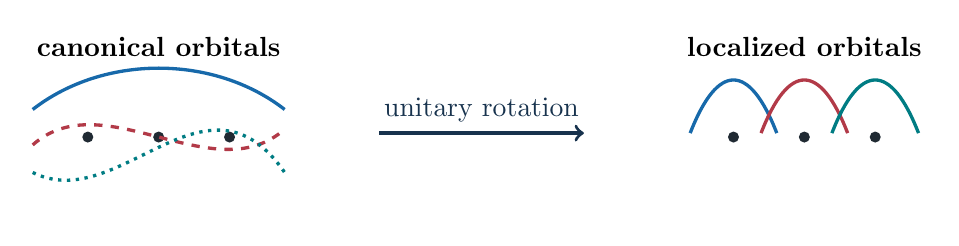
\begin{tikzpicture}[x=1cm,y=1cm]
		\node[font=\bfseries] at (-4.1,1.15) {canonical orbitals};
		\node[font=\bfseries] at ( 4.1,1.15) {localized orbitals};
		\foreach \x in {-5.0,-4.1,-3.2}{\fill[hfInk] (\x,0) circle (0.07);}
		\draw[hfBlue,very thick] (-5.7,0.35) .. controls (-4.8,1.05) and (-3.4,1.05) .. (-2.5,0.35);
		\draw[hfRed,very thick,dashed] (-5.7,-0.10) .. controls (-4.8,0.70) and (-3.4,-0.70) .. (-2.5,0.10);
		\draw[hfTeal,very thick,dotted] (-5.7,-0.45) .. controls (-4.6,-1.00) and (-3.5,1.00) .. (-2.5,-0.45);
		\draw[hfNavy,very thick,->] (-1.3,0.05)--(1.3,0.05)
			node[midway,above] {unitary rotation};
		\foreach \x in {3.2,4.1,5.0}{\fill[hfInk] (\x,0) circle (0.07);}
		\draw[hfBlue,very thick] (2.65,0.05) .. controls (3.0,0.95) and (3.4,0.95) .. (3.75,0.05);
		\draw[hfRed,very thick] (3.55,0.05) .. controls (3.9,0.95) and (4.3,0.95) .. (4.65,0.05);
		\draw[hfTeal,very thick] (4.45,0.05) .. controls (4.8,0.95) and (5.2,0.95) .. (5.55,0.05);
	\end{tikzpicture}

	\alert{Only occupied--occupied or virtual--virtual rotations are invariant;
	mixing occupied and virtual orbitals changes the determinant.}
\end{frame}

%-----------------------------------------------------
\begin{frame}{Localization fixes the unitary freedom by optimizing a criterion}
	A localization procedure selects one representative from all equivalent
	occupied-orbital sets:
	\begin{equation}
		\boxed{
			\bU_\star
			=
			\underset{\bU^\dagger\bU=\bI}{\operatorname{arg\,max}}
			\mathcal{L}(\bC_\text{o}\bU)
		}
	\end{equation}

	Most algorithms repeatedly rotate pairs of orbitals:
	\begin{equation}
		\begin{pmatrix}
			\widetilde{\psi}_p\\
			\widetilde{\psi}_q
		\end{pmatrix}
		=
		\begin{pmatrix}
			\cos\theta & \sin\theta\\
			-\sin\theta & \cos\theta
		\end{pmatrix}
		\begin{pmatrix}
			\psi_p\\
			\psi_q
		\end{pmatrix}.
	\end{equation}

	\begin{block}{Jacobi-sweep localization}
		\begin{enumerate}
			\item Choose an orbital pair $(p,q)$
			\item Determine the angle $\theta$ that improves $\mathcal{L}$
			\item Rotate the pair and continue through all pairs
			\item Repeat the sweeps until $\mathcal{L}$ is converged
		\end{enumerate}
	\end{block}

	Modern implementations may instead optimize directly on the unitary manifold.

	\vfill
	\centering
	\alert{The localization functional is generally nonconvex: different initial
	guesses may converge to different local extrema.}
\end{frame}

%-----------------------------------------------------
\begin{frame}{Boys orbitals minimize their spatial extent}
	For orbital $p$, define its centroid and quadratic spread:
	\begin{align}
		\bR_p
		&=
		\mel{\psi_p}{\br}{\psi_p},
		&
		\Omega_p
		&=
		\mel{\psi_p}{r^2}{\psi_p}
		-
		\abs{\bR_p}^2.
	\end{align}

	Boys localization minimizes the total spread,
	\begin{equation}
		\boxed{
			\Omega_\text{Boys}
			=
			\sum_p^\text{occ}
			\left[
				\mel{\psi_p}{r^2}{\psi_p}
				-
				\abs{\mel{\psi_p}{\br}{\psi_p}}^2
			\right]
			\quad\longrightarrow\quad\min
		}
	\end{equation}

	Because $\sum_p\mel{\psi_p}{r^2}{\psi_p}$ is invariant under occupied
	rotations, this is equivalent to separating the orbital centroids as much as possible.

	\begin{columns}[T,onlytextwidth]
		\begin{column}{0.48\textwidth}
			\begin{block}{Strengths}
				\begin{itemize}
					\item Simple geometric interpretation
					\item Requires only one-electron position integrals
					\item Produces compact bonds and lone pairs
				\end{itemize}
			\end{block}
		\end{column}
		\begin{column}{0.48\textwidth}
			\begin{block}{Limitations}
				\begin{itemize}
					\item Does not explicitly preserve $\sigma/\pi$ separation
					\item Centroids depend directly on molecular geometry
					\item Diffuse virtual orbitals may be difficult to localize
				\end{itemize}
			\end{block}
		\end{column}
	\end{columns}
\end{frame}

%-----------------------------------------------------
\begin{frame}{Pipek--Mezey orbitals maximize atomic localization}
	Associate an atomic population $q_A^{(p)}$ with orbital $p$. The original
	Pipek--Mezey criterion maximizes
	\begin{equation}
		\boxed{
			\mathcal{L}_\text{PM}
			=
			\sum_p^\text{occ}\sum_A
			\left(q_A^{(p)}\right)^2
			\quad\longrightarrow\quad\max
		}
	\end{equation}

	Using Mulliken populations for real orbitals,
	\begin{equation}
		q_A^{(p)}
		=
		\sum_{\mu\in A}\sum_\nu
		C_{\mu p}C_{\nu p}S_{\mu\nu}.
	\end{equation}

	\begin{columns}[T,onlytextwidth]
		\begin{column}{0.48\textwidth}
			\begin{block}{Chemical character}
				\begin{itemize}
					\item Maximizes the extent to which each orbital belongs to a few atoms
					\item Often preserves the separation between $\sigma$ and $\pi$ orbitals
					\item Produces intuitive bonds, lone pairs, and core orbitals
				\end{itemize}
			\end{block}
		\end{column}
		\begin{column}{0.48\textwidth}
			\begin{block}{Population analysis matters}
				The original Mulliken form can be basis-set dependent.
				L{\"o}wdin populations or intrinsic atomic orbitals provide more robust alternatives.
			\end{block}

			\begin{block}{Intrinsic bond orbitals}
				IBOs apply a Pipek--Mezey-like localization to populations defined in the
				intrinsic atomic-orbital basis.
			\end{block}
		\end{column}
	\end{columns}
\end{frame}

%-----------------------------------------------------
\begin{frame}{Different localization criteria answer different questions}
	Edmiston--Ruedenberg localization maximizes the sum of orbital self-repulsions:
	\begin{equation}
		\boxed{
			\mathcal{L}_\text{ER}
			=
			\sum_p^\text{occ}(pp|pp)
			\quad\longrightarrow\quad\max
		}
	\end{equation}

	\centering
	\small
	\renewcommand{\arraystretch}{1.30}
	\begin{tabularx}{0.96\textwidth}{
		>{\bfseries\raggedright\arraybackslash}m{0.18\textwidth}
		>{\raggedright\arraybackslash}m{0.25\textwidth}
		>{\raggedright\arraybackslash}m{0.22\textwidth}
		>{\raggedright\arraybackslash}X
	}
		\toprule
		Method & Optimized quantity & Main appeal & Main caution \\
		\midrule
		Boys
		& Spatial variance
		& Geometrically compact
		& No explicit atomic or $\sigma/\pi$ criterion
		\\
		Pipek--Mezey
		& Atomic populations
		& Chemically intuitive; often preserves $\sigma/\pi$
		& Depends on the population definition
		\\
		Edmiston--Ruedenberg
		& Self-Coulomb repulsion
		& Strong introrbital localization
		& More expensive because ERIs must be transformed
		\\
		IAO/IBO
		& Intrinsic atomic populations
		& Stable chemical interpretation
		& Requires construction of an intrinsic minimal basis
		\\
		\bottomrule
	\end{tabularx}

	\bigskip
	\alert{There is no universally \emph{best} localized orbital set: the criterion
	should match the intended interpretation or computational use.}
\end{frame}

%-----------------------------------------------------
\begin{frame}{Localization changes the representation, not the HF state}
	\begin{columns}[T,onlytextwidth]
		\begin{column}{0.48\textwidth}
			\begin{block}{What remains unchanged}
				\begin{itemize}
					\item The occupied subspace and Slater determinant
					\item The density matrix and electron density
					\item The HF energy and molecular properties
					\item The zero occupied--virtual Fock block
				\end{itemize}
			\end{block}

			\begin{block}{Why localize?}
				\begin{itemize}
					\item Identify bonds, lone pairs, and fragments
					\item Enable local correlation and embedding methods
					\item Select active spaces and domains
					\item Construct Wannier functions in periodic systems
				\end{itemize}
			\end{block}
		\end{column}
		\begin{column}{0.48\textwidth}
			\begin{block}{What changes}
				Localized orbitals are generally not Fock eigenfunctions:
				\begin{equation}
					\widetilde{\bF}_\text{oo}
					=
					\bU^\dagger\cdot\bepsilon_\text{o}\cdot\bU,
				\end{equation}
				which is not diagonal in general. Individual canonical orbital energies
				cannot therefore be assigned to localized orbitals.
			\end{block}

			\begin{block}{Practical cautions}
				\begin{itemize}
					\item Localize occupied and virtual spaces separately
					\item Core and valence orbitals are often localized separately
					\item Check for multiple extrema and discontinuous solutions
					\item Apparent point-group symmetry may be lost
				\end{itemize}
			\end{block}
		\end{column}
	\end{columns}

	\vfill
	\centering
	\pub{S.~F.~Boys, Rev. Mod. Phys. \textbf{32}, 296 (1960); C.~Edmiston and K.~Ruedenberg, Rev. Mod. Phys. \textbf{35}, 457 (1963).}

	\pub{J.~Pipek and P.~G.~Mezey, J. Chem. Phys. \textbf{90}, 4916 (1989); G.~Knizia, J. Chem. Theory Comput. \textbf{9}, 4834 (2013).}
\end{frame}

%-----------------------------------------------------
\subsection{Classification}
%-----------------------------------------------------

\begin{frame}{Stuber-Paldus classification of Hartree-Fock solutions}
	\footnotesize
	\centering
	\setlength{\tabcolsep}{2.5pt}
	\renewcommand{\arraystretch}{1.35}

	\begin{tabular}{
		@{}
		>{\centering\arraybackslash}m{0.16\textwidth}
		>{\centering\arraybackslash}m{0.21\textwidth}
		>{\centering\arraybackslash}m{0.18\textwidth}
		>{\centering\arraybackslash}m{0.40\textwidth}
		@{}
	}
		\rowcolor{hfPale}
		\makecell{\textbf{Fukutome}\\\textbf{designation}}
		&
		\makecell{\textbf{Stuber-Paldus}\\\textbf{designation}}
		&
		\makecell{\textbf{Symmetries}\\\textbf{preserved}}
		&
		\makecell{\textbf{Structure of the orbital}\\
		          \textbf{coefficient matrix $\bC$}}
		\\[0.5ex]

		$\mathrm{TICS}^{a}$
		&
		real RHF
		&
		$\chS^2,\,\chS_z,\,\chK,\,\hat{\Theta}$
		&
		$\mqty(
		\bC_{\sigma\sigma} & \bO
		\\
		\bO & \bC_{\sigma\sigma}
		),
		\quad \bC \in \mathbb{R}$
		\\

		$\mathrm{CCW}^{b}$
		&
		complex RHF
		&
		$\chS^2,\,\chS_z$
		&
		$\mqty(
		\bC_{\sigma\sigma} & \bO
		\\
		\bO & \bC_{\sigma\sigma}
		)\phantom{, \quad \bC \in \mathbb{R}}$
		\\

		$\mathrm{ASCW}^{c}$
		&
		paired UHF
		&
		$\chS_z,\,\hat{\Theta}$
		&
		$\mqty(
		\bC_{\sigma\sigma} & \bO
		\\
		\bO & \bC_{\sigma\sigma}^{*}
		)\phantom{, \quad \bC \in \mathbb{R}}$
		\\

		$\mathrm{ASDW}^{d}$
		&
		real UHF
		&
		$\chS_z,\,\chK$
		&
		$\mqty(
		\bC_{\sigma\sigma} & \bO
		\\
		\bO & \bC_{\sigma'\sigma'}
		),
		\quad \bC \in \mathbb{R}$
		\\

		$\mathrm{ASW}^{e}$
		&
		complex UHF
		&
		$\chS_z$
		&
		$\mqty(
		\bC_{\sigma\sigma} & \bO
		\\
		\bO & \bC_{\sigma'\sigma'}
		)\phantom{, \quad \bC \in \mathbb{R}}$
		\\

		$\mathrm{TSCW}^{f}$
		&
		paired GHF
		&
		$\hat{\Theta}$
		&
		$\mqty(
		\bC_{\sigma\sigma} & \bC_{\sigma\sigma'}
		\\
		-\bC_{\sigma\sigma'}^{*} & \bC_{\sigma\sigma}^{*}
		)\phantom{, \quad \bC \in \mathbb{R}}$
		\\

		$\mathrm{TSDW}^{g}$
		&
		real GHF
		&
		$\chK$
		&
		$\mqty(
		\bC_{\sigma\sigma} & \bC_{\sigma\sigma'}
		\\
		\bC_{\sigma'\sigma} & \bC_{\sigma'\sigma'}
		),
		\quad \bC \in \mathbb{R}$
		\\

		$\mathrm{TSW}^{i}$
		&
		complex GHF
		&
		{}
		&
		$\mqty(
		\bC_{\sigma\sigma} & \bC_{\sigma\sigma'}
		\\
		\bC_{\sigma'\sigma} & \bC_{\sigma'\sigma'}
		)\phantom{, \quad \bC \in \mathbb{R}}$
	\end{tabular}
	\\
	\flushleft
	$^a$ Time-reversal invariant closed-shell. 
	$^b$ Charge current wave. 
	$^c$ Axial spin current wave. 
	$^d$ Axial spin density wave. 
	$^e$ Axial spin wave. 
	$^f$ Torsional spin current wave. 
	$^g$ Torsional spin density wave.
	$^h$ Torsional spin wave.
\end{frame}

\begin{frame}{Stuber-Paldus classification of Hartree-Fock solutions}
	\center
	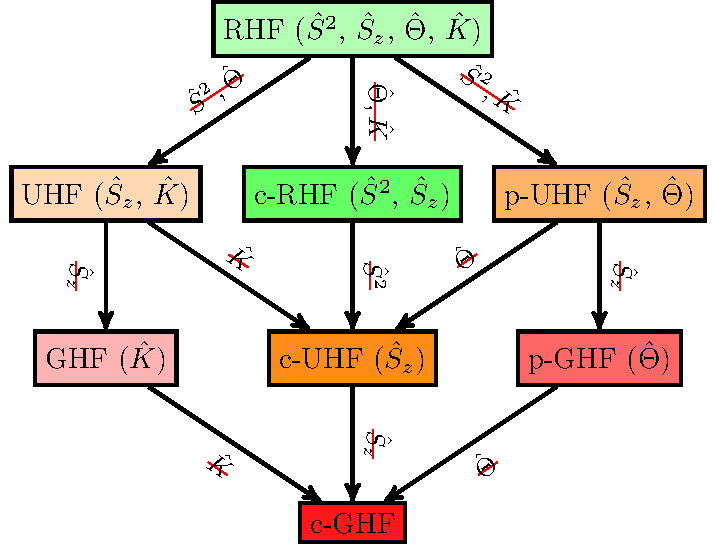
\includegraphics[width=0.66\textwidth]{fig/StuberPaldus}
\end{frame}

\begin{frame}{Generalized Hartree-Fock}
	GHF allows every orbital to choose its spin direction.
	A generalized Hartree--Fock orbital is a two-component spinor:
	\begin{equation}
		\boxed{
			\chi_p^\text{GHF}(\bx)
			=
			\alpha(\omega)\,\blue{\psi_p^\alpha(\br)}
			+
			\beta(\omega)\,\red{\psi_p^\beta(\br)}
		}
	\end{equation}
	Both components are expanded in the same spatial AO basis,
	\begin{equation}
		\psi_p^\sigma(\br)=\sum_{\mu=1}^{K}C_{\mu p}^\sigma\phi_\mu(\br)
		\qq{with}
		\bC=\mqty(\bC^\alpha\\[0.2em]\bC^\beta)
		\qand
		\bC\in\mathbb{C}^{2K\times N}
	\end{equation}

	\begin{columns}[T,onlytextwidth]
		\begin{column}{0.31\textwidth}
			\begin{block}{RHF}
				Paired electrons share one spatial orbital. Both $\chS^2$ and $\chS_z$ are preserved.
			\end{block}
		\end{column}
		\begin{column}{0.31\textwidth}
			\begin{block}{UHF}
				Each orbital is purely $\alpha$ or $\beta$. The spin density is collinear and $\chS_z$ is preserved.
			\end{block}
		\end{column}
		\begin{column}{0.31\textwidth}
			\begin{block}{GHF}
				Each orbital may mix $\alpha$ and $\beta$. In general, neither $\chS^2$ nor $\chS_z$ is preserved.
			\end{block}
		\end{column}
	\end{columns}

	\vfill
	\alert{GHF does not require a common spin-quantization axis or fixed values of $N^\alpha$ and $N^\beta$.}
\end{frame}

%-----------------------------------------------------
\begin{frame}{Spin mixing appears in the off-diagonal density blocks}
	For occupied GHF spinors, the density matrix is
	\begin{equation}
		\boxed{
			\bP=
			\mqty(
				\bP^{\alpha\alpha} & \bP^{\alpha\beta}\\
				\bP^{\beta\alpha} & \bP^{\beta\beta}
			)
		}
		\qq{with}
		P_{\mu\nu}^{\sigma\sigma'}
		=
		\sum_{i=1}^{N}C_{\mu i}^{\sigma}C_{\nu i}^{\sigma' *}
	\end{equation}

	\begin{columns}[T,onlytextwidth]
		\begin{column}{0.47\textwidth}
			\begin{block}{Charge and magnetization}
				At each point in space, the spin-density matrix $\boldsymbol{\gamma}(\br)$ gives
				\begin{align}
					n(\br) &= \operatorname{Tr}_s\boldsymbol{\gamma}(\br),\\
					m_k(\br) &= \operatorname{Tr}_s\!\left[\boldsymbol{\gamma}(\br)\sigma_k\right],
					\qquad k=x,y,z,
				\end{align}
				where $\sigma_k$ are the Pauli matrices and $\bs(\br)=\boldsymbol{m}(\br)/2$.
			\end{block}
		\end{column}
		\begin{column}{0.49\textwidth}
			\begin{block}{What do the blocks mean?}
				\begin{itemize}
					\item $\bP^{\alpha\alpha}+\bP^{\beta\beta}$ determines the charge density
					\item $\bP^{\alpha\alpha}-\bP^{\beta\beta}$ gives the $z$ component of magnetization
					\item $\bP^{\alpha\beta}$ and $\bP^{\beta\alpha}$ generate the transverse $x$ and $y$ components
				\end{itemize}
			\end{block}
		\end{column}
	\end{columns}

	\begin{equation}
		\text{UHF: }\bP^{\alpha\beta}=\bP^{\beta\alpha}=\bO
		\qquad\Longrightarrow\qquad
		\boldsymbol{m}(\br)\parallel\be_z.
	\end{equation}
	\alert{A state is collinear if one global spin rotation makes the transverse magnetization vanish everywhere.}
\end{frame}

%-----------------------------------------------------
\begin{frame}{The GHF equations are Roothaan--Hall equations in spinor space}
	The AO overlap is duplicated in spin space,
	\begin{equation}
		\overline{\bS}=\mqty(\bS&\bO\\\bO&\bS),
		\qquad
		\boxed{\bF\bC=\overline{\bS}\bC\bepsilon},
		\qquad
		\bC^\dagger\overline{\bS}\bC=\bI.
	\end{equation}

	For a spin-independent nonrelativistic Hamiltonian,
	\begin{equation}
		\boxed{
		\bF=
		\mqty(
		\bH+\bJ[\bP^0]-\bK[\bP^{\alpha\alpha}]
		& -\bK[\bP^{\alpha\beta}]\\
		-\bK[\bP^{\beta\alpha}]
		& \bH+\bJ[\bP^0]-\bK[\bP^{\beta\beta}]
		)
		}
	\end{equation}
	with $\bP^0=\bP^{\alpha\alpha}+\bP^{\beta\beta}$ and
	\begin{align}
		J[\bP]_{\mu\nu}
		&=\sum_{\lambda\kappa}P_{\lambda\kappa}(\mu\nu|\kappa\lambda),
		&
		K[\bP]_{\mu\nu}
		&=\sum_{\lambda\kappa}P_{\lambda\kappa}(\mu\lambda|\kappa\nu).
	\end{align}

	\begin{block}{SCF procedure}
		Build all four density blocks $\rightarrow$ build all four Fock blocks
		$\rightarrow$ solve a $2K\times2K$ generalized eigenvalue problem
		$\rightarrow$ occupy the $N$ lowest spinors $\rightarrow$ iterate.
	\end{block}

	\alert{The off-diagonal exchange blocks couple the $\alpha$ and $\beta$ components self-consistently.}
\end{frame}

%-----------------------------------------------------
\begin{frame}{GHF enlarges the variational space by releasing spin constraints}
	\centering
	\begin{equation}
		\boxed{
			\{\Phi_\text{RHF}\}
			\subset
			\{\Phi_\text{UHF}\}
			\subset
			\{\Phi_\text{GHF}\}
		}
		\qquad\Longrightarrow\qquad
		E_\text{GHF}\leq E_\text{UHF}\leq E_\text{RHF}
	\end{equation}
	for the corresponding global minima in the same one-electron basis.

	\begin{columns}[T,onlytextwidth]
		\begin{column}{0.48\textwidth}
			\begin{block}{A new stability direction}
				A converged UHF determinant may still be unstable to occupied--virtual rotations that mix $\alpha$ and $\beta$ orbitals. Following such a negative-curvature direction produces a lower-energy GHF solution.
			\end{block}

			\begin{block}{Not every GHF solution is noncollinear}
				RHF and UHF are special cases of GHF. A global spin rotation of a UHF determinant changes its apparent quantization axis but remains physically collinear.
			\end{block}
		\end{column}
		\begin{column}{0.48\textwidth}
			\begin{block}{Symmetry dilemma}
				Lowering the variational energy may require breaking exact symmetries:
				\begin{itemize}
					\item UHF may break $\chS^2$
					\item GHF may break both $\chS^2$ and $\chS_z$
					\item Complex GHF may also break time-reversal symmetry
				\end{itemize}
			\end{block}
		\end{column}
	\end{columns}

	\vfill
	\alert{A lower broken-symmetry HF energy does not imply a more faithful spin eigenfunction.}
\end{frame}

%-----------------------------------------------------
\begin{frame}{A triangular antiferromagnet naturally favors noncollinear spins}
	Consider three equivalent local moments with antiferromagnetic coupling,
	\begin{equation}
		E_\text{spin}=J\sum_{A<B}\boldsymbol{m}_A\cdot\boldsymbol{m}_B,
		\qquad J>0.
	\end{equation}

	\begin{columns}[T,onlytextwidth]
		\begin{column}{0.45\textwidth}
			\begin{block}{Collinear compromise}
				Two moments can be antiparallel, but the third bond must be frustrated:
				\begin{equation}
					\uparrow\;\downarrow\;\uparrow
					\qquad\Rightarrow\qquad
					\sum_{A<B}\boldsymbol{m}_A\cdot\boldsymbol{m}_B=-m^2.
				\end{equation}
				This pattern can be represented by UHF.
			\end{block}
		\end{column}
		\begin{column}{0.51\textwidth}
			\begin{block}{$120^\circ$ noncollinear solution}
				Let the three moments lie in a plane at angles $0^\circ$, $120^\circ$, and $240^\circ$:
				\begin{align}
					\boldsymbol{m}_A+\boldsymbol{m}_B+\boldsymbol{m}_C&=\bO,\\
					\boldsymbol{m}_A\cdot\boldsymbol{m}_B
					=\boldsymbol{m}_B\cdot\boldsymbol{m}_C
					=\boldsymbol{m}_C\cdot\boldsymbol{m}_A&=-\frac{m^2}{2},\\
					\sum_{A<B}\boldsymbol{m}_A\cdot\boldsymbol{m}_B&=-\frac{3m^2}{2}.
				\end{align}
				All three bonds share the frustration equally. GHF can represent this texture with one determinant.
			\end{block}
		\end{column}
	\end{columns}

	\alert{Equilateral $\ce{H3}$ and triangular magnetic clusters are useful classroom examples of genuine noncollinearity.}
\end{frame}

%-----------------------------------------------------
\begin{frame}{GHF is useful when spin direction is part of the physics}
	\small
	\begin{columns}[T,onlytextwidth]
		\begin{column}{0.48\textwidth}
			\begin{block}{Typical applications}
				\begin{itemize}
					\item Geometrically frustrated antiferromagnets
					\item Polyradicals, fullerenes, and magnetic clusters
					\item Zeeman fields and spin-dependent one-electron Hamiltonians
					\item Two-component treatments including spin--orbit coupling
					\item Broken-symmetry references for spin projection or nonorthogonal CI
				\end{itemize}
			\end{block}
		\end{column}
		\begin{column}{0.48\textwidth}
			\begin{block}{Interpret with care}
				\begin{itemize}
					\item GHF is still a single determinant: correlation is not restored
					\item $S$ and $M_S$ are generally not good quantum numbers
					\item Local moments may be artifacts for an exact singlet
					\item Many stationary solutions make the initial guess important
					\item Complex algebra and a doubled matrix dimension increase the cost
				\end{itemize}
			\end{block}
		\end{column}
	\end{columns}

	\begin{block}{Take-home message}
		GHF is the most general number-conserving single-determinant HF ansatz. It is best viewed as a flexible broken-symmetry representation whose physical content should be checked through spin densities, stability analysis, and--when needed--symmetry restoration.
	\end{block}
%
%	\vspace{0.25em}
%	\centering
%	{\scriptsize\textcolor{hfPurple}{H.~Fukutome, Int. J. Quantum Chem. \textbf{20}, 955 (1981); J.~J.~Goings \textit{et al.}, Int. J. Quantum Chem. \textbf{118}, e25398 (2018).}}

%	{\scriptsize\textcolor{hfPurple}{C.~A.~Jim\'enez-Hoyos \textit{et al.}, J. Phys. Chem. A \textbf{118}, 9925 (2014); S.~Sun \textit{et al.}, J. Chem. Theory Comput. \textbf{15}, 348 (2019).}}
\end{frame}

%-----------------------------------------------------
\section{Books}
%-----------------------------------------------------
\begin{frame}{Recommended references}
	\begin{columns}
		\begin{column}{0.7\textwidth}
			\begin{itemize}
				\item Introduction to Computational Chemistry (Jensen)
				\\
				\vspace{1cm}
				\item Essentials of Computational Chemistry (Cramer)
				\\
				\vspace{1cm}
				\item Modern Quantum Chemistry (Szabo \& Ostlund)
				\\
				\vspace{1cm}
				\item Molecular Electronic Structure Theory (Helgaker, J{\o}rgensen \& Olsen)
				\\
				\vspace{1cm}
			\end{itemize}
		\end{column}
		\begin{column}{0.3\textwidth}
				\centering
				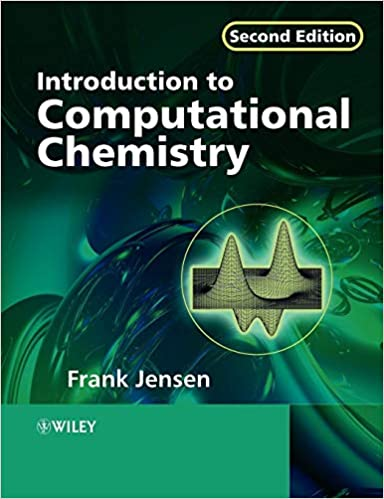
\includegraphics[height=0.3\textwidth]{fig/Jensen}
				\\
				\bigskip
				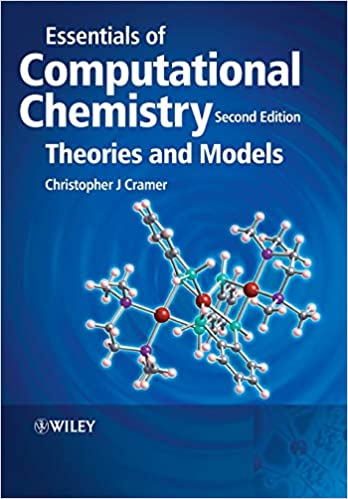
\includegraphics[height=0.3\textwidth]{fig/Cramer}
				\\
				\bigskip
				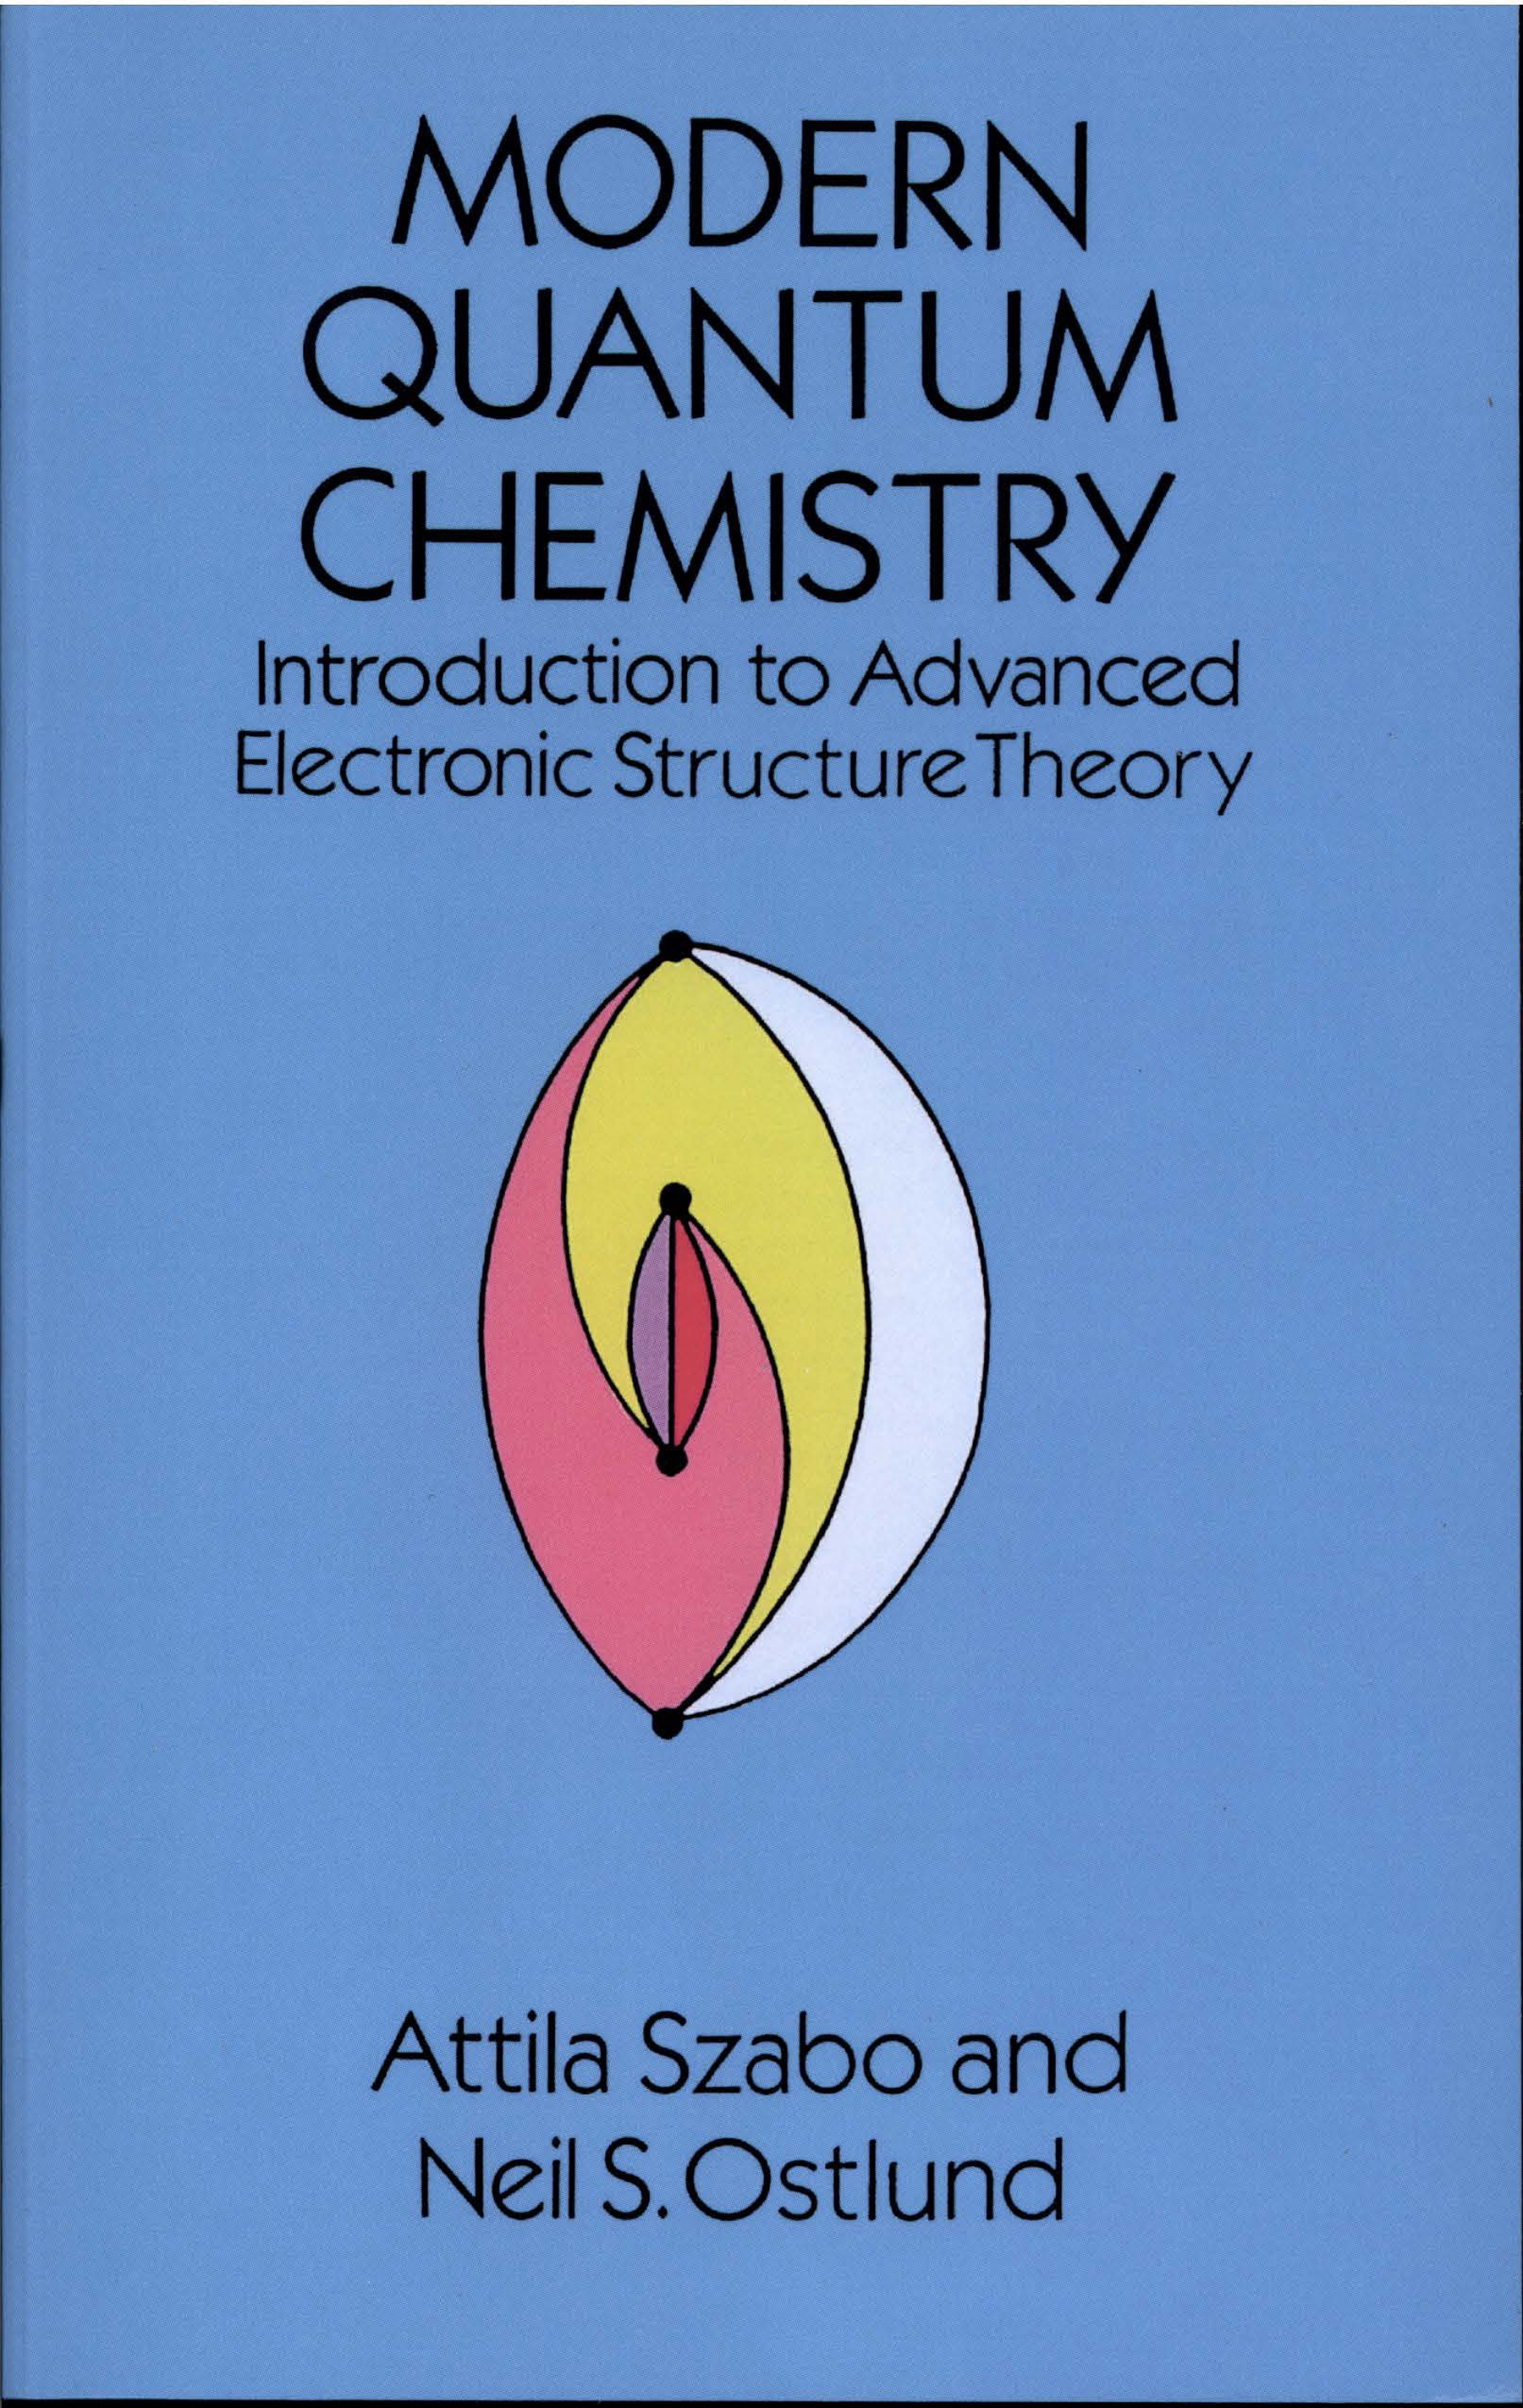
\includegraphics[height=0.3\textwidth]{fig/Szabo}
				\\
				\bigskip
				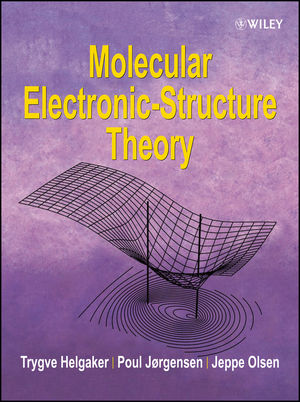
\includegraphics[height=0.3\textwidth]{fig/Helgaker}
		\end{column}
	\end{columns}
\end{frame}

\end{document}
